\documentclass{_main_paper}

\journal{Transportation Research Part E}

\setlength{\parindent}{14pt}
\setlength{\parskip}{0em}

\begin{document}
\begin{frontmatter}


\title{Optimization Model for Large-Scale Long-term Aircraft Maintenance Scheduling and Station Assignment at American Airlines}

% Authors
% \author[1]{JohnPaul Adimonyemma}
% \ead{johnpaul1.adimonyemm@famu.edu}
% \author[1]{Yanshuo Sun\texorpdfstring{\corref{cor1}}{}}
% \ead{y.sun@eng.famu.fsu.edu}
% \texorpdfstring{\cortext[cor1]{Corresponding author}}{Corresponding author}
% \address[1]{Department of Industrial and Manufacturing Engineering, FAMU-FSU College of Engineering, Florida Agricultural and Mechanical University, Tallahassee, FL, US}

\address{[Blinded Manuscript]}


% \input{sections/0_abstract}

\begin{abstract}
The primary focus of the existing aircraft maintenance optimization literature is on short-term aircraft maintenance routing. By contrast, only a few studies address long-term maintenance planning, which predominantly emphasize scheduling decisions: none of them have examined the critical aspect of assigning aircraft to maintenance stations, a key challenge for major airlines with a network of maintenance facilities. Additional research gaps include (1) insufficient consideration of practical maintenance-related constraints (e.g., station access limit and aircraft rotation requirement) and (2) the absence of scalable algorithms capable of solving real-world problem instances involving hundreds of aircraft and dozens of maintenance stations. To fill those gaps, this study introduces a joint optimization model for aircraft maintenance scheduling and station assignment to assist a U.S.-based airline in creating long-term plans for a fleet of over 800 aircraft of multiple subfleet types. To address the computational challenges, we propose two decomposition approaches: one based on decision types and the other on time horizons. Extensive computational experiments using real-world data demonstrate that these approaches can reduce computation time by up to 80\% with a minimal increase in the optimization objective (less than 2\%). The proposed model is expected to streamline maintenance planning efforts and enhance outcomes for aircraft maintenance professionals.
\end{abstract}



\begin{keyword}
Aircraft maintenance, Scheduling and assignment, OR in airlines, Decomposition approaches, Case studies
\end{keyword}

\end{frontmatter}

\clearpage

\newpage

\section{Introduction} 
Aviation is one of the safest means of transportation compared to other modes, primarily due to the prioritization of safety by airlines over other key performance indicators \citep{chen2024advancing}. Aircraft operations in civil aviation are meticulously regulated by government agencies, such as the Federal Aviation Administration (FAA) in the U.S. and the European Union Aviation Safety Agency (EASA), among others. Violating safety regulations and policies imposed by those aviation authorities leads to the grounding of aircraft and other more severe penalties. All major airlines have thus established their aircraft maintenance programs to ensure each aircraft is safe to operate and meets all applicable regulatory requirements. While aircraft safety is essential, it comes with a significant financial burden, as maintaining aircraft is known to be very expensive.
Based on cost data collected from airlines across the globe, the International Air Transport Association (IATA) estimated that airlines worldwide spent over \$76 billion on Aircraft Maintenance, Repair, and Overhaul (MRO) in 2022 only, which accounted for nearly 11\% of the total airline operating cost \citep{iata2022mcx}. By contrast, the IATA projected that the airline net profit margin would improve to 2.7\% in 2024, a slight increase over 2.6\% in 2023 \citep{iata2023pressrelease}.
Consequently, while aircraft maintenance is crucial, it is also costly, necessitating proper planning to minimize costs and improve airline profitability while ensuring compliance with all regulatory requirements.

Many transportation and operations researchers have contributed to the critical research area of aircraft maintenance optimization. A comprehensive review of the literature, provided in Section~\ref{section:liteReview}, reveals that most existing studies focus on the aircraft maintenance routing problem. By contrast, only a handful have addressed how a fleet of aircraft should be maintained over an extended planning horizon, namely the long-term aircraft maintenance planning problem.
Key distinctions exist between these two major groups of studies (i.e., aircraft maintenance routing vs long-term aircraft maintenance planning) in terms of the planning period and the nature of maintenance activities analyzed. 
Regarding the planning horizon length, aircraft maintenance routing problems involve a short planning period (such as a week), whereas long-term aircraft maintenance problems span over multiple months or years. Regarding the nature of maintenance activities, short-term aircraft maintenance routing problems focus on routine and minor checks \citep{sriram2003optimization,liang2009aircraft}, while long-term aircraft maintenance problem addresses major checks such as C checks or D checks \citep{van2013aircraft}.
Given the practical need of a collaborating airline (which remains anonymous), we focus on the long-term aircraft maintenance planning problem in this paper.

Considering the existing studies on the long-term aircraft maintenance problem, we have identified three major shortcomings through a detailed literature review in Section~\ref{section:liteReview}.
First, existing studies in this area have focused mainly on the scheduling of aircraft for maintenance checks. As a result, only scheduling decisions have been optimized. For instance, \cite{deng2020practical} optimized long-term maintenance scheduling for A and C checks over a three-year period at a single maintenance station.  However, in the real-world practice for a major airline with a network of maintenance stations, long-term planning often requires both the scheduling of aircraft and the assignment to different maintenance stations. Jointly optimizing these decisions (i.e., scheduling and station assignment) remains crucial for effective maintenance planning, which should be done to fill an important gap. 
Second, we observe that most existing studies have considered only basic maintenance-related constraints, such as man-hour limits, while neglecting many other practical constraints. For instance, these studies failed to account for station-specific limits on the number of C or A checks (referred to as C check and A check limits, respectively), aircraft rotation requirement, station access limit, and the possibility of conducting multiple checks for a single aircraft over a planning period.
Third, the problem sizes addressed in existing studies on the long-term planning problem have been limited. While small-scale problems can be solved directly using commercial solvers, this direct solution approach becomes impractical as the problem size increases. To address this, some researchers have developed heuristic solution approaches. However, the quality of solutions produced by these heuristic approaches is unclear.


To address the research gaps identified above, we first develop a long-term aircraft maintenance optimization model that determines when and where an aircraft should be scheduled for maintenance. Many practical constraints specified by the collaborating U.S. airline (namely American Airlines or AA) have been considered, such as two C checks in the same group could be conducted on an aircraft on the same day while C checks from different groups cannot be mixed. In addition to directly solving the integrated optimization model by a commercial solver, two decomposition-based solution approaches are proposed, namely a scheduling-first-assignment-second approach and a temporal decomposition approach. Extensive computational experiments are conducted based on real-world data to validate the effectiveness, efficiency, and practical usefulness of the long-term aircraft maintenance planning method.



This paper has made several major contributions. The first contribution is from the modeling perspective. This paper introduces the first integrated optimization model for aircraft maintenance scheduling and station assignment, involving a heterogeneous fleet of aircraft, a network of maintenance bases with different capabilities and capacities, and covering an extended planning horizon. The second contribution lies in the design of effective solution algorithms. This study proposes two novel decomposition-based solution approaches that can achieve a near-optimal solution with a relative gap of below 2\% while reducing computation time by up to 80\% compared to directly solving the mixed integer program with a commercial solver. Finally, this paper presents a real-world aircraft maintenance planning case study that is larger in scale than any others in the current literature, measured by the fleet size, the number of maintenance facilities, and the number of maintenance capacity parameters. 




The remainder of this paper is described as follows. In Section~\ref{section:liteReview}, we review the literature on aircraft maintenance planning in civil aviation. In Section~\ref{Problem_definition_formulation}, we introduce the mixed integer programming formulation for the integrated aircraft maintenance scheduling and assignment problem, aiming to minimize the discounted maintenance costs over the planning horizon. In Section~\ref{section:solutionmethodology}, we present two different decomposition-based solution approaches to reduce the computation time. Case studies are conducted based on data from a U.S.-based airline, as described in Section~\ref{section:case_studies}. Finally, the findings and recommendations for future research directions are provided in Section~\ref{section:conclusions}.




\section{Literature Review} 
\label{section:liteReview}

The literature review is structured as in Figure \ref{fig:org_lit_review}. In Section \ref{aircraft_maint_practice}, we describe the general practice in aircraft maintenance and introduce relevant terminologies. Depending on the planning horizon length, there are two types of aircraft maintenance planning problems, namely short-term planning problems reviewed in Section \ref{aircraft_maint_practice} and long-term planning problems reviewed in Section \ref{aircraft_maint_practice}. As this paper is concerned with a large-scale joint optimization problem, we further review popular solution algorithms used to solve large-scale optimization problems, particularly the decomposition-based solution approaches with applications in aviation in Section \ref{sec:SolApproach}. Finally, major research gaps are summarized in Section \ref{sec:LitRevSummary}.


\begin{figure}[htbp]
    \centering
    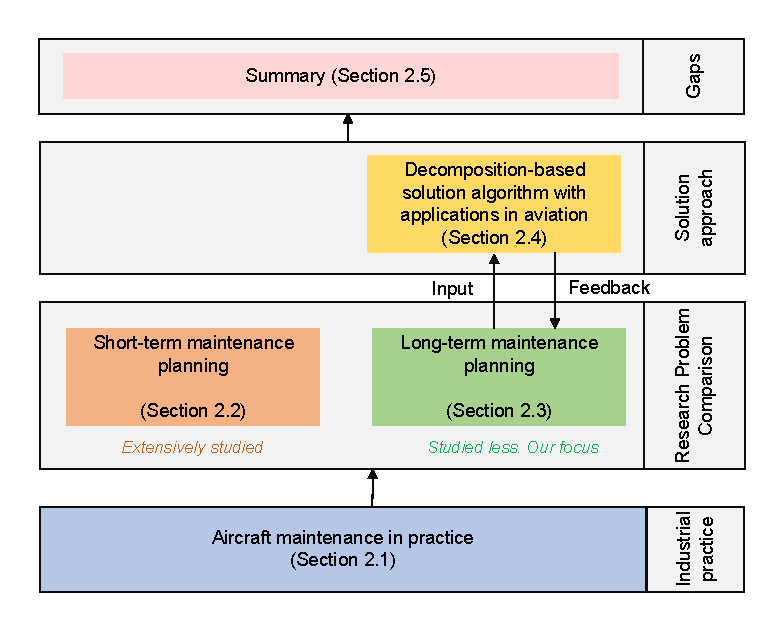
\includegraphics[width=0.65\linewidth]{literature_framework.pdf}
    \caption{Organization of the literature review}
    \label{fig:org_lit_review}
\end{figure}



\subsection{Aircraft maintenance in practice }
\label{aircraft_maint_practice}
In civil aviation, aircraft undergo various maintenance activities at predetermined intervals. These maintenance activities are generally classified as preventive (scheduled) or corrective (unscheduled). 
Preventive maintenance is a proactive process performed to prevent system failures \citep{van2013aircraft,tseremoglou2024condition}. This type of maintenance is organized into four key types of checks, commonly referred to as lettered checks: A, B, C, and D checks \citep{preventive_vs_on-condition}. The intervals for these checks are tracked using several indicators, including calendar days, flight cycles, and flight hours. These intervals are well defined in the maintenance program \citep{icao2019aircraft}. For instance, an A check is typically conducted every 600–2,000 flight hours, 200–300 flight cycles, or 60–150 calendar days. Many airlines have discontinued B checks to reduce the overlap with A checks \citep{lagos2020dynamic}. A new C check is due after approximately 16,000 flight hours, 2,000 flight cycles, or 24–26 months, while D checks, which are the most extensive, take place roughly every 6–10 years \citep{naatypesofaviationmaint}. Although in some studies, those checks are named A-check, B-check, and so on, we do not keep the hyphen between the letter and ``check'' to be consistent with the practice of the collaborating airline. \color{black} Depending on its fleet characteristics (such as mix and age), an airline usually creates its own maintenance program to address its specific needs. In contrast with preventative maintenance, corrective maintenance involves unscheduled tasks that are necessary to restore an aircraft system to optimal condition after a failure has occurred \citep{eddarhri2022towards}.

Depending on the maintenance location, aircraft maintenance can also be classified as line vs base (hangar) maintenance. Line maintenance refers to tasks carried out at the gate or on the apron.  Line maintenance activities usually occur during an aircraft's ground time window or are called ``maintenance opportunity'' \citep{villafranca2025aircraft}. \color{black}  Any maintenance work that cannot be completed in the above areas is classified as base or hangar maintenance \citep{van2013aircraft}. The execution of these maintenance tasks largely depends on an airline's capabilities. Some airlines carry out maintenance in-house at their own facilities, often located in airport hangars, while others choose to outsource the work to third-party MRO providers.


\subsection{Short-term maintenance planning for aircraft}
\label{subsect:maint_routin_problm}
To better understand the maintenance planning problem, we briefly discuss the airline scheduling process and then focus on the short-term problem variants, particularly the well-studied aircraft maintenance routing problem (AMRP) and the line maintenance scheduling problem (LMSP). 
\color{black}


There are four types of scheduling problems in airline operations, namely flight scheduling, fleet assignment, aircraft maintenance routing, and crew scheduling, which are solved sequentially \citep{barnhart2004airline}.
As illustrated in Figure~\ref{fig:airline_scheduling problem}, the airline scheduling process begins with flight scheduling, at least a few months in advance. In this stage, an airline identifies the markets to serve, the frequency of flights, and the timing of these flights. Once flight schedules are established, specific aircraft types are assigned to flight legs of the identified schedules during the fleet assignment process \citep{clarke1997aircraft}. Many factors, such as aircraft capacity, range, and fuel efficiency, are considered during fleet assignment to match the most suitable aircraft type with each flight leg \citep{gopalan1998aircraft}. Following fleet assignment, aircraft maintenance routing deals with the assignment of each individual aircraft to flight legs. A rotation is a series of flight legs with the destination of a leg as the origin of the immediate next leg, while the final destination is the same as the initial origin of an aircraft, thus completing a tour. While completing the rotation, an aircraft is mandated to visit certain maintenance facilities according to maintenance regulations. Additionally, in crew scheduling, airlines assign crew members (flight attendants and pilots) to flight legs. 


\begin{figure}[htbp]
    \centering
    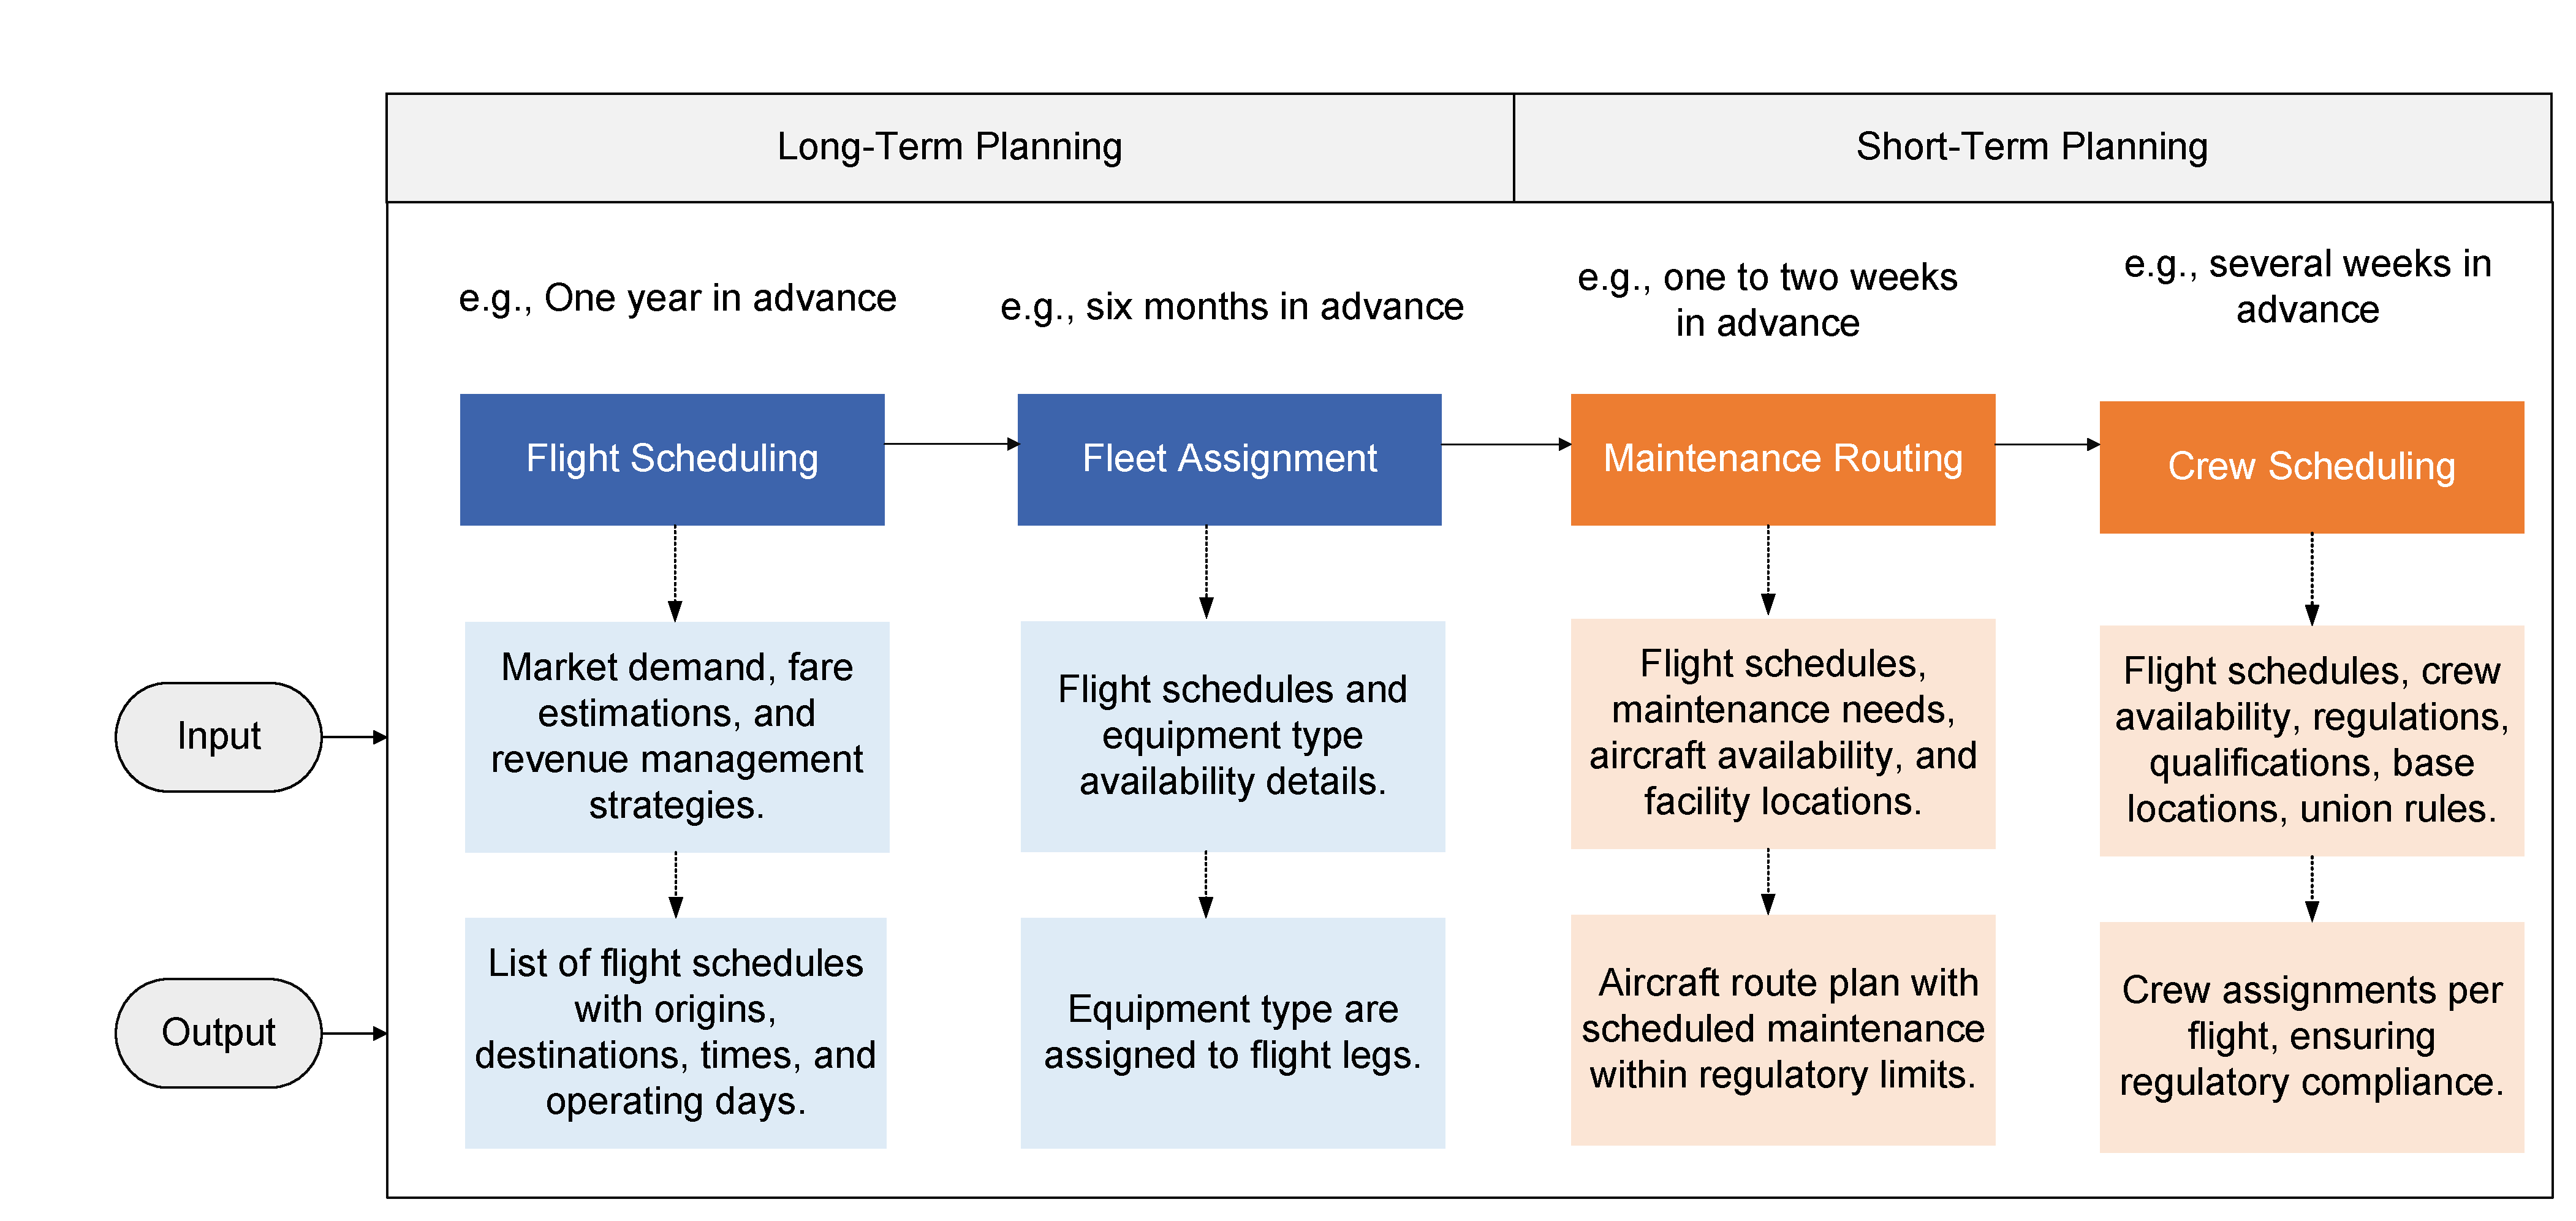
\includegraphics[width=\linewidth]{airlineschedulingv7.pdf}
    \caption{Overview of an airline scheduling process}
\label{fig:airline_scheduling problem}
\end{figure}

Although all the above four optimization problems have been widely studied in the literature, we next focus on the AMRP, considering the relevance of the AMRP to our research. 
Given \color{black} a set of aircraft and corresponding flight schedules, the AMRP is concerned with assigning aircraft to sequences of flights (referred to as ``routes'') while ensuring both operational and maintenance requirements are met. This means that a suitable aircraft must cover every flight leg, and necessary maintenance must be performed without disrupting scheduled operations. Typically, the planning horizon for AMRP usually spans two to four days \citep{feo1989flight, eltoukhy2017airline}, though in some cases, it may extend up to a week \citep{sriram2003optimization, he2023maximizing}. 
We further briefly comment on the size of AMRP instances. For example, \cite{ruan2021reinforcement} considered nine real-world instances from Egyptair. The number of flight legs varies from 40 to 400; the fleet size varied from 8 to 42; the number of maintenance stations involved ranged from 4 to 9. 



In addition to the AMRP, we further review other short-term aircraft maintenance planning problems without involving aircraft routing. In an LMSP study, \cite{villafranca2025aircraft} focused on deciding what maintenance tasks should be outsourced versus performed in-house and determining the start times for these in-house tasks.
The study specifically examined line maintenance operations carried out during maintenance opportunities, with a planning horizon of 24 hours.



\subsection{Long-term maintenance planning for aircraft}
\label{sec:long_termPlanningRev}

While the planning horizon in short-term maintenance planning problems is typically no more than several weeks, the long-term aircraft maintenance planning problem is defined over a much longer time horizon, spanning several months or even years \citep{ma2022tackling}. The differing planning horizon length implies a few other key differences. First, in the AMRP, detailed flight departure and arrival times are known and a series of flight legs are built into an aircraft route; by contrast, detailed flight schedules are unavailable for an extended planning horizon, such as six months, no aircraft routing decisions are involved in a long-term aircraft maintenance planning study. 
Second, due to AMRP's short-term nature, it primarily considers routine checks that occur quite frequently, e.g., once every a few days \citep{sriram2003optimization}. By contrast, the long-term aircraft maintenance planning usually involves major checks, such as the C checks that are needed infrequently (e.g., once every a few months).

Given the above differences, we present an in-depth review of only those studies focusing on long-term planning problems.


\cite{boere1977air} documented innovative efforts made by Air Canada in the 1970s to replace a manual procedure for long-term aircraft maintenance scheduling with the Aircraft Maintenance Operations Simulation (AMOS) model. AMOS was essentially a simulation system where a priority-based scheduling heuristic was incorporated, because \cite{boere1977air} argued that other modeling or solution approaches, including mixed integer programming, dynamic programming, and out-of-kilter algorithms, were unsuitable. Their optimization objective was to minimize the lost aircraft flying hours and it was concluded that a 5\% maintenance cost and labor reduction was achieved. A related study \cite{deng2020practical} followed six major conditions for maintenance scheduling, originally introduced in \cite{boere1977air}, and made two more assumptions. They sought to determine whether a check for an aircraft should start on a given day over a long planning horizon (such as four years), following a dynamic programming (DP) framework. They tested their solution method in a case study based in Europe, which involved a fleet of 45 A320 aircraft. A single maintenance base was considered, as they focused on scheduling decisions only. The DP approach might face computer memory issues for large instances. 


% However, several extensions to \cite{deng2020practical} work were made, and we discussed them as follows.  
We next review a few studies built upon \cite{deng2020practical}. \cite{andrade2021aircraft} 
utilized a Deep Q-learning algorithm to optimize long-term maintenance scheduling policies developed by  \cite{deng2020practical}. Their methodology prioritized the schedule of C checks over A checks, given that C checks require more ground time and significantly influenced the scheduling of subsequent A checks. 
Rather than minimizing maintenance costs, they focused on maximizing flight utilization between two consecutive checks to increase aircraft availability in the long term. The test instances involved in this analysis were the same as those of \cite{deng2020practical}.
Their experimental results demonstrated that reinforcement learning produced a more efficient maintenance plan than dynamic programming adopted by \cite{deng2020practical}.
\color{black}
\cite{van2022robust} developed an integer programming model to generate a long-term heavy maintenance schedule for checks, which comprises the C and the D checks. Given a sequence of C checks, the D is merged with the C check, which is carried out after every two C cheeks have been scheduled. Their main decision was to determine the start of a maintenance check for a particular aircraft. Given the increase in complexity, they solved the optimization problem using a genetic algorithm (GA) that was validated on synthetic aircraft maintenance data. \cite{van2022robust}  ran the DP solution approach developed by  \cite{deng2020practical}, and then compared the results of GA with that of DP. In terms of the practicality of the model, they considered some applicable constraints such as utilization, maintenance, and operational constraints. However, they did not consider explicitly some practical capacity constraints at the maintenance stations, such as the man hours available at the station. A single maintenance station was considered. 

Rather than merely focusing on check scheduling only,  \cite{deng2020practical} further incorporated task allocation and shift planning into a decision support system (DSS). \color{black} The DSS took input from multiple sources, such as the maintenance planning document, fleet status, operational constraints, task workload, and workforce availability. It employed a top-down optimization approach in which, at the task allocation level, it focused on allocating tasks to a maintenance opportunity. 
% A maintenance opportunity, as defined by \cite{deng2021novel}, is a given time window for performing a specific check with corresponding capacity. 
However, the DSS did not consider aircraft-to-station assignment as it considered only a single maintenance station. In addition, the DSS only considered the general man-hour capacity constraints available at their maintenance hangar. However, given the supposed practicality of this framework, other necessary real-world capacity constraints, such as the number of checks a station can handle (line count limit) and the possibility of handling two C checks per day or combining both A and C checks and so on, remain vital. 

Other long-term maintenance planning studies are also reviewed. Focusing on maintenance schedules for Taiwan's major airline operator and its client's fleet,
\cite{yan2008long} presented an integer programming model for the long-term aircraft maintenance planning considering a single airport, with multiple hangars, and a heterogeneous fleet. Their core decision was when an aircraft should be assigned for maintenance at which hangar. Over their planning horizon, each aircraft needed at most one check. Therefore, they explicitly defined a single maintenance due date for an aircraft. They did not specify where A and/C checks were conducted in their study. If A checks were involved, there should be multiple A checks over a one-year period, while their model was unable to address that. Their optimization model was solved directly by a commercial solver (CPLEX) after two objectives were merged into one with a weighting method. As their case study involved 68 aircraft and one airport, they did not design any custom solution algorithms to address larger problem instances. 


We present the summary of these studies for long-term aircraft maintenance planning problem in Table~\ref{tab:sum_aircraft_maint}. We further comment that many practical constraints, such as aircraft rotation requirement, A check limit, C Check limit, and station access limit, are absent in those existing long-term studies. In addition, the preference of an aircraft to be maintained at a particular station, which is preferred by major airlines, has not been considered in those existing studies.  It should be noted that all those studies in Table~\ref{tab:sum_aircraft_maint} considered a single maintenance station, although a major airline will likely use multiple maintenance stations when its fleet is sufficient large.


\begin{table}[htbp]
\centering
\caption{Summary of long-term aircraft maintenance planning studies}
\label{tab:sum_aircraft_maint}
\resizebox{\textwidth}{!}{%
% \fontsize{14}{20}\selectfont
\begin{tabular}{lccccccl}
\hline
\multirow{3}{*}{Study} & \multirow{3}{*}{Data type} & \multirow{3}{*}{\begin{tabular}[c]{@{}c@{}}Maintenance \\ check type\end{tabular}} & \multirow{3}{*}{\begin{tabular}[c]{@{}c@{}}Number of \\ maintenance \\ check types\end{tabular}} & \multirow{3}{*}{\# of stations} & \multirow{3}{*}{\begin{tabular}[c]{@{}c@{}}Aircraft \\ fleet size\end{tabular}} & \multirow{3}{*}{Fleet type} & \multirow{3}{*}{Solution approach} \\
 &  &  &  &  &  &  &  \\
 &  &  &  &  &  &  &  \\ \hline
\cite{boere1977air} & R & A,B,C & 3 & 1 & - & HT &  Simulation-based heuristic \\
\cite{yan2008long} & R & - & - & 1 & 68 & HT &  Exact Algorithm \\
\cite{deng2020practical} & R & A,C & 2 & 1 & 45 & HM & Dynamic Programming \\
\cite{deng2021novel} & R & A,C & 2 & 1 & 66 & HM &  Worst-Fit Decreasing Algorithm \\
\cite{andrade2021aircraft} & R & A,C & 2 & 1 & 45 & HM & Deep Q-learning \\
\cite{van2022robust} & S & C,D & 2 & 1 & 40 & - &  Genetic Algorithm \\
\textbf{Our work} & \textbf{R} & \textbf{A,C01-C10} & \textbf{11} & \textbf{15} & \textbf{$>$800} & \textbf{HT} &  \textbf{Decomposition-based  Approaches} \\ \hline
\end{tabular}%
}
\begin{minipage}{\textwidth} 
    \footnotesize
    \vspace{1mm}
    R - Real-world data;$\quad$ S - Simulated data; $\quad$
     HT - Heterogeneous Fleet;$\quad$
     HM - Homogeneous Fleet
 \end{minipage}
\end{table}


As shown in Table~\ref{tab:sum_aircraft_maint}, existing studies addressing long-term aircraft maintenance planning problems have all been conducted on a small to medium-sized scale. This is evident from the limited number of aircraft (fewer than 70), and the number of maintenance stations (limited to only one).
% , and the parameters defining maintenance capacity.
Given that solving these problems using exact methods with commercial solvers has become impractical even for these small-scale problems as a result of complexities, fast heuristics are usually developed to tackle these problems \citep{wang2024collaboration}.

We note that some seemingly relevant studies are not reviewed in detail, as they focus on a more granular level. For example, \cite{chen2024resource} broke down a single C check of an aircraft into hundreds of maintenance tasks and aimed to optimize the task scheduling to minimize the makespan (i.e., the duration of the C check). Given the focus of \cite{chen2024resource} on a single check, it is not directly relevant to the core research problem of this paper. 


\subsection{Decomposition-based solution algorithm with applications in aviation}
\label{sec:SolApproach}
% As shown in Table~\ref{tab:sum_aircraft_maint}, previous studies addressing long-term aircraft maintenance planning problems have all been conducted on a small to medium-sized scale. This is evident from the limited number of aircraft (fewer than 70), the number of maintenance stations (limited to only one), and the parameters defining maintenance capacity. Given that solving these problems using exact methods with commercial solvers has become impractical for these small scale problems, some studies have developed heuristic solution approaches, 
% to tackled these problems. However, they remain impractical when the problem size grows. For instance, \cite{deng2020practical} observed that although dynamic programming can yield exact solutions, it suffers from the curse of dimensionality, rendering it impractical for large-scale instances due to excessive computational requirements.


As no studies have tackled the joint optimization of aircraft maintenance scheduling and station assignment decisions in the literature, no applicable solution algorithms are available. To motivate the solution algorithm design for the long-term aircraft maintenance optimization problem under consideration in this paper, we briefly review several common decomposition-based solution strategies for solving large-scale optimization problems in aviation. 
For instance, \cite{sama2013rolling} utilized the rolling horizon decomposition approach to determine aircraft scheduling while considering busy traffic situations resulting from a large number of delayed aircraft. They achieved this by updating the scheduling decision based on new traffic information. 
In contrast, \cite{diao2018sequence} adopted a different decomposition solution approach by using a hybrid decomposition method that combines Dantzig-Wolfe decomposition and column generation for air traffic management. Similarly, \cite{wang2025airport} developed a customized decomposition approach that hierarchically separates strategic flight scheduling from operational adjustments to solve the airport slot allocation problem. 



\color{black}
\subsection{Summary}
\label{sec:LitRevSummary}
Although the literature on aircraft maintenance optimization is extensive, the vast majority of the current literature is devoted to the short-term planning problem, which is different from the long-term aircraft maintenance planning problem in terms of the planning horizon length and type of decisions involved. An in-depth review of the handful long-term aircraft maintenance planning studies produces the following research gaps:
\begin{enumerate}
    \item The existing long-term aircraft maintenance planning studies have focused primarily on the timing of maintenance checks and have not incorporated aircraft-to-station assignments.
    For major airlines with a large set of spatially distributed maintenance facilities, aircraft-to-station assignment decisions (where to conduct maintenance) are as necessary as the scheduling decision (when to conduct maintenance). 
    % For a major airline operating a large fleet and a network of maintenance facilities, the joint optimization of two interrelated decisions, namely scheduling (when to conduct maintenance) and assignment (where to conduct maintenance) is essential. 
    At present, none of the existing studies have attempted to optimize them jointly and address the above practical need,  possibly because jointly optimizing them is quite challenging.
    \item Although some maintenance-related constraints, such as man-hour limits, are considered in the existing aircraft maintenance planning studies, many practical constraints remain unaddressed. For example, each maintenance station is constrained by the number of aircraft it can accommodate, referred to as the line count. The number of C checks that can be performed on an aircraft is 0, 1, or 2, while C checks from different groups cannot be carried out simultaneously.
    The aircraft rotation constraint is also missing in the existing aircraft maintenance planning studies. Those constraints should be considered to improve the realism of aircraft maintenance planning. 
    \item The current studies on the long-term aircraft maintenance planning problem have primarily focused on small to medium-sized problems. For instance, the maximum fleet size is less than 100 in the current literature while a major airline may operate hundreds of aircraft in the real world. As a result, the solution approaches developed for these problems might be inadequate for large, realistic problem instances.
\end{enumerate}

To address the identified research gaps, a practical integrated optimization method for aircraft maintenance scheduling and assignment at a large scale is essential, which is presented in this study.  
\section{Mathematical Formulation} 
\label{Problem_definition_formulation}
\subsection{Problem Definition}
A fleet of aircraft is represented by the set $I$, with each aircraft uniquely identified by a tail number $i \in I$. As many different aircraft types (such as Boeing vs Airbus, or wide-body vs narrow-body) are involved in the fleet, the set of all subfleet types, such as 737-800 and A320-Neo, is denoted as $S$. Among all aircraft in fleet $I$, those of subfleet type $s$ are collectively denoted as set $I_s$. Each subfleet type is associated with a set of maintenance checks, or called checks, such as A and C. There are, in total, ten types of C checks (also called phase checks), which are divided into two groups by maintenance interval, namely C01-C06 and C07-C10. The first group is referred to as One-C phase checks, which are conducted more frequently than the phase checks in the second group, namely Two-C phase checks. 
The set of all check types is denoted as $K$. We next define an aircraft-check tuple $w=\left(i,k\right)$ or simply tuple $w$, where $i \in I$ and $k \in K_i$. It is noted that $K_i \subseteq K$ as aircraft $i$ is not required to complete all checks in $K$; only those checks in a subset $K_i$ apply to aircraft $i$.

The maintenance interval for tuple $w=\left(i,k\right)$ is denoted as $m_w$, essentially the maximum possible time (measured in days) between two consecutive checks of type $k$ for aircraft $i$. 
Right after a check is completed, the Days-To-Go or DTG becomes $m_w$,  and it drops by one every day. The initial DTG is denoted as $\delta_w^0$. The next check must be scheduled before the DTG drops to zero (as illustrated in Figure~\ref{fig:maint_cycle}). Otherwise, maintenance is overdue, which is strictly prohibited by FAA regulations. 
Figure~\ref{fig:maint_cycle}  shows and contrasts two possible scenarios: premature vs ideal. In the premature scenario, a check is completed before the DTG drops to the minimum (typically zero or one), and some usable days are then lost or wasted, leading to a yield of less than 100\%. In the ideal scenario, a check is completed on the check due date, and a yield of 100\% is obtained (i.e., zero waste).

% Figure~\ref{fig:maint_cycle} 
% illustrates that when a check is completed before the DTG drops to zero, some usable days are lost or wasted, leading to a yield of less than 100\%. When a check is completed on the check due date, a yield of 100\% is obtained (i.e., zero waste).


\begin{figure}[ht]
    \centering
    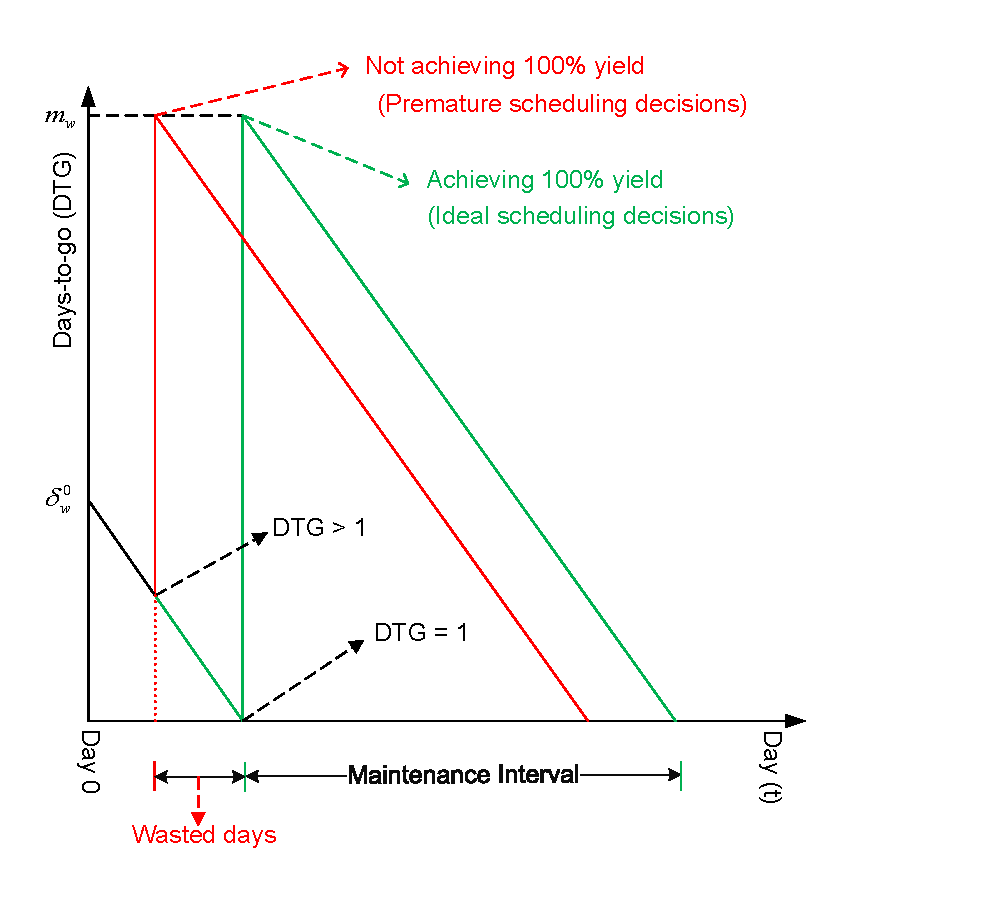
\includegraphics[width=0.65\linewidth]{Daystogo_v2.pdf}    
    \caption{Evolution of days-to-go for a tuple $w$}
    \label{fig:maint_cycle}
\end{figure}


To conduct various checks for all aircraft in the fleet, the airline owns and operates a set of maintenance stations, denoted as $J$. As a station $j \in J$ cannot service all aircraft types, we use $J_w$ to represent a subset of stations that are capable of servicing tuple $w$. Each station $j$ has a few capacity parameters. Specifically, the maximum man-hours available at station $j$ is given as $H_j$; the maximum number of A-checks station $j$ can complete daily is $A_j$; the number of phase checks at station $j$ is limited at $U_j$; the maximum number of phase checks that can be performed on a given aircraft at station $j$ is $R_j$; and the total number of aircraft to be maintained at a station is limited at $Q_j$ each day. When the above capacity parameters vary over time, a superscript $t$ is added. For instance, $H_j$ can be changed to $H_j^t$. Additionally, the number of aircraft of subfleet type $s$ that can access station $j$ on day $t$ for maintenance is limited as $P_{sj}^t$. Note that $\sum_s\sum_jP_{sj}^t$ could be much smaller than the fleet size $|I|$, because not all aircraft could access airports with maintenance capabilities every day. 

As a certain type of aircraft can be maintained at multiple stations, an aircraft has a preference for maintenance stations given its subfleet type due to factors related to routing convenience or historical performance record.  We thus define $\beta_{wj}$ to represent the preference of tuple $w$ for station $j$. For each tuple $w$, a more preferred station $j$ is associated with a lower $\beta_{wj}$, which can also be interpreted as a relative cost. Introducing $\beta_{wj}$ is expected to break the solution symmetry among stations. 

 
Given the fleet of aircraft $I$, its associated maintenance checks $K$, and a set of heterogeneous maintenance stations $J$, the airline seeks to determine on which day $t$ and at which station $j$, which type of check $k$ is scheduled for aircraft $i$. The objective is to minimize the discounted maintenance cost over the planning horizon. 
 

\subsection{Mixed Integer Programming Formulation}
\label{subsec:MIP_formulation}

\begingroup
\setstretch{1} % Set the line spacing to single within this group
\begin{longtable}{l p{16cm}}
\caption{Notation}
\label{tab:notation_tab} \\
\hline
\multicolumn{2}{l}{\textit{Sets and Indices}} \\ \hline
\endfirsthead
\multicolumn{2}{c}{{\tablename\ \thetable{} -- continued from previous page}} \\
\hline
\endhead
\endfoot
\hline
\endlastfoot
$I$ & Set of aircraft, indexed by $i$ \\
$J$ & Set of all maintenance stations, indexed by $j$ \\
$J_i$ & Set of maintenance stations capable of maintaining aircraft $i$ \\
$S$ & Set of all aircraft subfleet types, indexed by $s$ \\
$I_s$ & Set of all aircraft of subfleet type $s$, $I_s \subseteq I$ \\
$K$ & Set of all maintenance check types, indexed by $k$ \\
$K_i$ & Set of check types applicable to aircraft $i$, $K_i \subseteq K$ \\
$W$ & Set of $w = (i,k)$ tuples, where $i \in I$ and $k \in K_i$ \\
$W_i$ & Set of tuples specific to aircraft $i$, $W_i \subseteq W$ \\
$\bar{W}$ & Set of all tuples involving A checks, $\bar{W} \subseteq W$  \\
$\hat{W}$ & Set of all tuples involving One-C checks, $\hat{W} \subseteq W$ \\
$\hat{W}_i$ & Set of all tuples involving One-C checks for aircraft $i$, $\hat{W}_i \subseteq \hat{W} $\\
$\breve{W}$ & Subset of $W$ including all Two-C checks, $\breve{W} \subseteq W$ \\
$\breve{W_i}$ &  Set of all tuples involving Two-C for aircraft $i$, $\breve{W_i} \subseteq W$  \\
$J_w$ & Subset of stations capable of undertaking tuple $w$\\
$T$ & Planning horizon, i.e., a set of days $\left\{1,2,\dots,|T|\right\}$ \\
\hline
\multicolumn{2}{l}{\textit{Parameters}} \\ \hline
$m_w$ & Maximum allowable time (in days) between two consecutive checks for tuple $w$ \\
$\eta$ & Minimum number of days an aircraft must wait before visiting the same station for maintenance \\
$\delta_w^0$ & DTG for tuple $w$ at the beginning of the planning horizon \\
$P_{sj}^t$ & Maximum number of aircraft of subfleet type $s$ that can be routed to station $j$ on day $t$ \\
% $\gamma^t$ & Future cost discounting coefficient for day $t$ \\
$\gamma$ & A coefficient to be used in future cost discounting, e.g., 0.99  \\
$l_w$ & Man-hours needed for tuple $w$ \\
$M$ & Maximum number of checks that can be done daily for an aircraft, e.g., 2 or 3 \\
$\beta_{wj}$  & Relative cost of maintaining tuple $w$ at station $j$ to model an aircraft's station preference \\
$A_j^t$ & Number of A checks that can be accomplished at station $j$ on day $t$ \\
$H_j^t$ & Number of man-hours available at station $j$ on day $t$ \\
$Q_j^t$ & Number of distinct aircraft that station $j$ will handle on day $t$  \\
$U_j^t$ & Number of phase checks that can be accomplished at station $j$ on day $t$ \\
$R_j^t$ & Number of phase checks that can be performed simultaneously on a given aircraft at station $j$ on day $t$\\

\hline
\multicolumn{2}{l}{\textit{Decision Variables}} \\ \hline
$x_{wj}^t$ & A binary variable to be 1 if tuple $w$ is completed at station $j$ on day $t$. \\
$y_w^t$ & DTG for aircraft $i$ for check $k$ on day $t$ \\ 
$z_{ij}^t$ & A binary variable to be 1 if aircraft $i$ is assigned to station $j$ on day $t$ for maintenance \\
$\hat{\pi}_j^t$ & A binary variable to be 1 if station $j$ is open for One-C checks on day $t$ \\
$\breve{\pi}_j^t$ & A binary variable to be 1 if station $j$ is open for Two-C checks on day $t$ \\
\end{longtable}
\endgroup

Before the mathematical formulation is presented, some simplifying assumptions adopted in this study are stated here. First, we focus on a deterministic optimization problem, which means future uncertainty about man hours and other capacity parameters is not considered. Second, although maintenance can be driven by different time indicators (i.e., days-to-go, hours-to-go, and cycles-to-go), due to the lack of aircraft usage data (e.g., the number of flight hours by day), we model days-to-go only, without considering other time indicators. Nonetheless, we note that Eqs \eqref{eq:initial_day_to_go} to \eqref{eq:withinLimits_dtg} (to be presented later) can be modified for other indicators. Third, each maintenance check that is considered in this study can be conducted overnight, according to the collaborating airline.


% Before the mathematical formulation is presented, some simplifying assumptions adopted in this study are stated here: 
% \begin{enumerate}
%     \item We focus on a deterministic optimization problem, which means future uncertainty about man hours and other capacity parameters is not considered.
%     \item Although maintenance can be driven by different time indicators (i.e., days-to-go, hours-to-go, and cycles-to-go), due to the lack of aircraft usage data (e.g., the number of flight hours by day), we model days-to-go only, without considering other time indicators. Nonetheless, we note that Eqs \eqref{eq:initial_day_to_go} to \eqref{eq:withinLimits_dtg} (to be presented later) can be modified for other indicators.
%     \item The maintenance check that is considered in this study can be conducted overnight, according to the collaborating airline.
% \end{enumerate}

% \color{black}

With notation in Table~\ref{tab:notation_tab}, we now present the following mathematical program for the joint aircraft maintenance scheduling and assignment problem, which is abbreviated as JP (joint problem).
\begin{flalign}
\text{(JP)} \quad	\min_{\left\{x_{wj}^t, y_w^t, z_{ij}^t, \hat{\pi}_j^t, \breve{\pi}_j^t\right\}}  \quad  \quad  &  \sum_{w \in W}\sum_{j \in J_w}\sum_{t \in T} \gamma^t \beta_{wj} x_{wj}^t  \label{eq:ObjDaystogo} \\
% Assign stations to aircraft
	\text{s.t.}  \quad \quad   &\sum_{j \in J_w} x_{wj}^t \leq 1, \quad \forall w \in W, t \in T \label{eq:AtmostOneCheckPerDay} \\
%Days to go evolution
     &  y_w^1 =\delta_w^0, \quad \forall w \in W \label{eq:initial_day_to_go}\\
    & y_w^t \leq y_w^{t-1} - 1 + m_w \sum_{j \in J_w} x_{wj}^{t-1}, \quad \forall w \in W, t \in T \setminus \left\{1\right\} \label{eq:statusEvolution-dtg} \\
     \hspace{0.5em} & y_w^t \ge m_w \sum_{j \in J_w} x_{wj}^{t-1}, \quad \forall w \in W , t \in T \setminus \left\{1\right\} \label{eq:statusEvolution-dtgAdded} \\
    & y_w^t \ge y_w^{t-1} - 1, \quad \forall w \in W, t \in T \setminus \left\{1\right\}\label{eq:statusEvolution-dtg_2} \\
    & 1 \leq y_w^t \leq m_w, \quad \forall w \in W, t \in T  \label{eq:withinLimits_dtg} \\
%Routing Constraints
    &  \sum_{w \in W_i} x_{wj}^t \le M z_{ij}^t \quad \forall i \in I, j \in J, t \in T \label{eq:routingDepen} \\
%Capacity constraints
    &  \sum_{i \in I_s}z_{ij}^t  \leq P_{sj}^t, \quad \forall s \in S, j \in J, t \in T \label{eq:stationAccessbyw} \\
     & \sum_{w \in W}l_w x_{wj}^t  \leq H_j^t, \quad \forall j \in J, t \in T \label{eq:manhourcapacity}\\
    &\sum_{i \in I}z_{ij}^t \leq Q_j^t, \quad \forall j \in J, t \in T  \label{eq:checkwork_check_capacity} \\
     &  \sum_{j \in J_i} z_{ij}^t \le 1, \quad \forall i \in I, t \in T \label{eq:oneaircraft_perday2} \\
    &\sum_{w \in \bar{W}} x_{wj}^t\leq A_j^t, \quad \forall j \in J, t \in T \label{eq:station_Acheck_capacity}  \\
    & \hat{\pi}_j^t + \breve{\pi}_j^t  \leq 1, \quad \forall j \in J, t \in T  \label{eq:notsamephasechecktype} \\
    & \sum_{w \in\hat{W}}x_{wj}^t  \leq U_j^t\hat{\pi}_j^t, \quad \forall j \in J, t \in T  \label{eq:notsamephasechecktypeHat} \\
    & \sum_{w \in \breve{W}}x_{wj}^t  \leq U_j^t \breve{\pi}_j^t, \quad \forall j \in J, t \in T  \label{eq:notsamephasechecktypebreve} \\
     &  \sum_{w \in \hat{W_i}} x_{wj}^t + \sum_{w \in \breve{W_i}} x_{wj}^t \leq  R_j^t,   \quad \forall i \in I, j \in J, t \in T \label{eq:phasecheckperaircraft} \\
    &\sum_{{t^\prime} = t}^{t+ \eta - 1}  z_{ij}^{t^\prime} \le 1, \quad \forall i \in I, j \in J, t \in \left\{1, \ldots, |T| - \eta + 1 \right\} \label{aircraft_rotation}\\
    & x_{wj}^t \in \{0,1\},  \quad \forall w \in W, j \in J_w, t \in T \label{eq:JointBinary}\\
    & y_w^t \in R,  \quad \forall w \in W, t \in T \label{eq:JointBinary1} \\
     &z_{ij}^t \in \{0,1\},  \quad \forall i \in I, j \in J_i , t \in T\label{eq:JointBinary2} \\
      &\hat{\pi}_j^t \in \{0,1\},  \quad \forall j \in J , t \in T\label{eq:JointBinary3} \\
      &\breve{\pi}_j^t \in \{0,1\},  \quad \forall j \in J , t \in T\label{eq:JointBinary4} 
 \end{flalign}    


In the optimization objective Eq.~\eqref{eq:ObjDaystogo}, we seek to minimize the weighted maintenance cost over the planning horizon $T$.
Incorporating future cost discounting via $\gamma^t$ leads to the postponement of maintenance whenever feasible. We note that $\gamma^t$ is computed as $\gamma$ raised to the power of $t$, which decreases over time, thus achieving the aim of discounting future cost. \color{black} To illustrate the necessity of future cost discounting, we present a toy example where the goal is to determine the optimal time to schedule the next A check for a single aircraft, T020. There is one maintenance station with adequate capability and capacity, and the planning period spans from Day 1 to Day 30. The current DTG is 20, and the maintenance interval is 100 days. When aiming to minimize the number of checks, the next A check can be scheduled on any day between Day 1 and Day 19, before the DTG reaches its minimum. Performing the A check on any of these days yields the same optimization objective of 1. However, to avoid wasting useful days from the previous check, the latest possible day is preferred, which is achieved by considering future cost discounting through $\gamma^t$. Additionally, the inclusion of $\beta_{wj}$ is intended to assign tuple $w$ to its most preferred stations when possible.

Constraint~\eqref{eq:AtmostOneCheckPerDay} ensures that each tuple $w$ can be assigned to at most one station in $J_w$ on day $t$.
Constraint~\eqref{eq:initial_day_to_go} initializes the DTG for tuple $w$. Constraints~\eqref{eq:statusEvolution-dtg}, \eqref{eq:statusEvolution-dtgAdded}, \eqref{eq:statusEvolution-dtg_2}, and \eqref{eq:withinLimits_dtg} together model how DTG $y_w^t$ varies over time for every tuple $w$. 
When no checks are scheduled on day $t-1$, i.e., $\sum_{j \in J_w} x_{wj}^{t-1} = 0$, constraints~\eqref{eq:statusEvolution-dtg} and \eqref{eq:statusEvolution-dtg_2} together ensure $y_w^t$ decreases by exactly 1 from day $t-1$ to day $t$. 
When $\sum_{j \in J_w} x_{wj}^{t-1} = 1$, constraint~\eqref{eq:statusEvolution-dtgAdded} ensures $y_w^t$ is at least $m_w$ and constraint~\eqref{eq:withinLimits_dtg} imposes the upper bound $m_w$. In other words, when a maintenance occurs on $t-1$, $y_w^t$ is exactly $m_w$ (i.e., being reset) on day $t$, one day later. We further note that on the day of maintenance $t-1$, the smallest possible DTG is 1, which increases to exactly $m_w$ on the following day $t$.
Constraint~\eqref{eq:routingDepen} states that when aircraft $i$ is not routed to station $j$ on day $t$, no checks can be completed for aircraft $i$ at station $j$ on day $t$ due to aircraft $i$'s lack of access to station $j$. Note that $M$ stands for the maximum number of checks that can be completed for an aircraft at any given station each day, which is usually 2 or 3.
Constraint~\eqref{eq:stationAccessbyw} ensures that the number of aircraft that can be routed to station $j$ on the day $t$ is capped for each subfleet type $s$.
Constraint~\eqref{eq:manhourcapacity} ensures that the man-hour limit at station $j$ is not violated. 
Constraint~\eqref{eq:checkwork_check_capacity} ensures that the maximum number of aircraft that can be worked on day $t$ at station $j$ is not exceeded. 
Constraint~\eqref{eq:oneaircraft_perday2} ensures that an aircraft cannot visit different stations $j$ on the same day $t$ for maintenance.
Constraint~\eqref{eq:station_Acheck_capacity} ensures that the number of A-checks a station can handle is not exceeded. 
Constraint~\eqref{eq:notsamephasechecktype} ensures that at station $j$, aircraft $i$ can have only one type of phase checks; mixing One-C and Two-C checks is prohibited. Constraint~\eqref{eq:notsamephasechecktypeHat} enforces that unless station $j$ is open for One-C checks on day $t$, no One-C tuples could be scheduled. Constraint~\eqref{eq:notsamephasechecktypebreve} enforces a similar requirement, but for Two-C checks.
Constraints~\eqref{eq:notsamephasechecktypeHat} and \eqref{eq:notsamephasechecktypebreve} also enforce that the number of phase checks a station can accommodate, namely $U_j$, is not exceeded.
Constraint~\eqref{eq:phasecheckperaircraft} ensures that the total number of phase checks performed on aircraft $i$ is not exceeded at station $j$.
Constraint~\eqref{aircraft_rotation} ensures that when an aircraft $i$ visits maintenance station $j$, it cannot visit it again for maintenance in the next $\eta$ days after the visit, to avoid aircraft routing complexities. More specifically, constraint~\eqref{aircraft_rotation} prevents two visits by an aircraft $i$ to the same station $j$ over a period from $t$ to $t + \eta -1$, a brief period consisting of $\eta$ days. This is because it is very difficult to create a series of flight segments to bring an aircraft to the same station with small amount of time such as $\eta$ days.
Constraints~\eqref{eq:JointBinary}, \eqref{eq:JointBinary2}, \eqref{eq:JointBinary3}, and \eqref{eq:JointBinary4} define $x_{wj}^t$, $z_{ij}^t$, $\hat{\pi}_j^t$, and $\breve{\pi}_j^t$  as binary variables, respectively. 
Constraint~\eqref{eq:JointBinary1} defines $y_w^t$ as a real number even though at the optimality, $y_w^t$ is an integer, which is bounded in constraint~\eqref{eq:withinLimits_dtg}.

Planning decisions made on the final day of horizon $T$ are subject to distortion, as the consequences beyond the planning horizon are not considered. Specifically, for tuples with a DTG of exactly one (the minimum allowable value) on Day $|T|$, no maintenance is scheduled on Day $|T|$. This outcome arises for two key reasons. First, leaving these tuples unscheduled on Day $|T|$ does not violate any feasibility constraints within the planning horizon $T$. Second, if maintenance were scheduled for these tuples on Day $|T|$, their DTG would reset, however, on Day $|T| + 1$, which is outside of Horizon $T$. Those checks scheduled on Day $|T|$, unfortunately, worsen the optimization objective, defined solely over Horizon $T$. 
This phenomenon, caused by the finite nature of the planning horizon, is formally stated in  
Proposition~\ref{lem:EndOfHorizon}. 

\begin{lem}
\label{lem:EndOfHorizon}
The formulation given by Eqs.~\eqref{eq:ObjDaystogo} to \eqref{eq:JointBinary4} exhibits an End-of-Horizon effect, where no tuples are planned for maintenance on the last day of horizon $T$.
\end{lem}

\begin{proof}
We prove this by contradiction. We assume that $x_{\bar{w},j}^{|T|} = 1$ at the optimality, where tuple $\bar{w}$ has a DTG of one, i.e., $y_{\bar{w}}^t = 1$. 
 Then, reducing $x_{\bar{w},j}^{|T|}$ to zero leads to a strictly smaller objective value as given by Eq.~\eqref{eq:ObjDaystogo} while not causing any constraints to become infeasible. This implies that $x_{\bar{w},j}^{|T|} = 1$ cannot hold at optimality, contracting the initial assumption. Thus, the proof is completed. 
\end{proof}

\subsection{Preprocessing of Set of Tuples}

It should be noted that the set of tuples $W$ could be replaced by a subset of it, which only includes those tuples satisfying $\delta_w^0 \leq |T| + \epsilon$, where $\epsilon$ is a buffer, e.g., 15 days. This condition prevents clearly premature maintenance checks. Intuitively, for a tuple with an initial DTG of $\delta_w^0$, its DTG will not drop to zero at the end of the planning horizon $T$, if the above condition is met. Then, tuple $w$ does not need to undergo a check over horizon $T$. This preprocessing technique can significantly reduce the cardinality of set $W$, thus reducing the problem size and computation time. Therefore, this preprocessing technique is adopted in all case studies presented later.

We further note that for any given planning horizon, many checks with longer maintenance intervals can be excluded with the above preprocessing. For instance, for a planning horizon of 180 days, all tuples concerned with A checks should be kept as A checks have an interval of less than 180 days. By contrast, some C checks can be excluded if their initial DTGs are substantially greater than 180. \color{black}

\section{Decomposition-based Solution Approaches}
\label{section:solutionmethodology}
The aircraft maintenance scheduling and assignment problem Eqs.~\eqref{eq:ObjDaystogo} to \eqref{eq:JointBinary4} presented in Section~\ref{Problem_definition_formulation} is a mixed integer program, which can be solved with a commercial solver when the problem scale is limited. However, this problem has a very large scale for realistic instances. This is evident as both the number of variables and constraints grow rapidly as the problem size increases. For instance, the number of variables $x_{wj}^t$ increases with the number of tuples $|W|$, number of stations $|J|$, and number of days in the planning horizon $|T|$. Similarly, the number of constraints also grows with the number of stations and/or the planning horizon length. This observation motivates us to decompose a large-scale scheduling and assignment problem into smaller and more manageable sub-problems. Specifically, we seek to explore two decomposition strategies: (1) separating assignment from scheduling and (2) temporal decomposition.

In Section~\ref{sec:SchedulingThenAssign}, we first describe a scheduling-first-assignment-second solution approach; in Section~\ref{sec:tempDecomp}, we seek to achieve the temporal decomposition with a rolling horizon approach.

 


% \subsection{Scheduling-then-Assigning Approach}
\subsection{Sequential Heuristic (SH) Approach}
\label{sec:SchedulingThenAssign}
In the base formulation Eqs.~\eqref{eq:ObjDaystogo} to \eqref{eq:JointBinary4}, we jointly optimize the scheduling and assignment decisions. We now explore a decomposition-based heuristic by sequentially optimize scheduling and assignment decisions. In the scheduling stage, no information about individual maintenance stations is available; only the aggregated capacity parameters are known. In the assignment stage, all optimization decisions made during the scheduling stage are known as inputs and the new decision is to assign tuples to stations day by day.

Table~\ref{tab:notation_tabDecomp} shows some additional notation used in the decomposition approach. Note that the notation in Table~\ref{tab:notation_tab} remains applicable.


% \usepackage{array}


\begin{table}[ht]
\centering
\caption{Notation used in the scheduling-only problem}
\label{tab:notation_tabDecomp}
\begin{tabular}{lp{16cm}} 
\toprule
\multicolumn{2}{l}{\textit{Parameters}} \\ 
\hline
$\bar{P}_{s}^t$ & Maximum number of aircraft of subfleet type $s$ that can be routed to any maintenance stations on day $t$, $\bar{P_{s}^t} =\sum_{j\in J}P_{sj}^t$ \\
$\bar{H}^t$ & Maximum man-hours available on day $t$, $\bar{H}^t =\sum_{j\in J}H_j^t$ \\
$\bar{Q}^t$ & Number of distinct aircraft that a station can handle on day $t$ for maintenance, $\bar{Q}^t =\sum_{j\in J}Q_j^t$ \\
$\bar{U}^t$ & Maximum number of phase checks that can be accomplished on day $t$, $\bar{U} =\sum_{j\in J}U_j^t$ \\
$R^\prime$ & Maximum number of phase checks that can be performed simultaneously on a given aircraft at any station daily, $\hat{R} = \max_j\left\{R_j^t\right\}$ \\
$e_i^t$ & A binary parameter to indicate if at least one of the maintenance stations that can complete multiple phase check has nonzero station access for aircraft $i$ on day t \\
$\bar{A}^t$ & Maximum number of A-checks that can be accomplished on day $t$, $\bar{A} =\sum_{j\in J} A_j^t$ \\
$\bar{I}$ & Set of aircraft needing phase checks \\ 
$\bar{I_s}$ &  Set of all aircraft of subfleet type $s$ needing phase checks \\ 
\hline
\multicolumn{2}{l}{\textit{Decision Variables}} \\ 
\hline
$x_w^t$ & A binary variable to be 1 if tuple $w$ is scheduled for day $t$ \\
$y_w^t$ & Days-to-go for aircraft $i$ for check $k$ on day $t$ \\
$z_i^t$ & A binary variable to be 1 if aircraft $i$ is scheduled for maintenance on day $t$ \\
$\hat{\psi}_i^t$ & A binary variable to be 1 if One-C Phase Check is scheduled on day $t$ for aircraft $i$ \\
$\breve{\psi}_i^t$ & A binary variable to be 1 if Two-C Phase Check is scheduled on day $t$ for aircraft $i$ \\ \bottomrule
\end{tabular}
\end{table}
% \newpage

By dropping aircraft-to-station assignment decisions from the joint optimization problem Eqs.~\eqref{eq:ObjDaystogo} to \eqref{eq:JointBinary4}, we have the following scheduling-only problem (SOP) using additional notation in Table~\ref{tab:notation_tabDecomp}:
\begin{flalign}
\text{(SOP)} \quad	\min_{\left\{x_{w}^t, y_w^t,z_i^t,\hat{\psi}_i^t,\breve{\psi}_i^t \right\}}  \quad  \quad  &  \sum_{w \in W}\sum_{t \in T} \gamma^t x_{w}^t  \label{eq:ObjDaystogoSub} \\
    %Days to go evolution
    \text{s.t.}  \quad \quad &  y_w^1 =\delta_w^0, \quad \forall w \in W \label{eq:initial_day_to_gosub}\\
    & y_w^t \leq y_w^{t-1} - 1 + m_w x_{w}^{t-1}, \quad \forall w \in W, t \in T \setminus \left\{1\right\} \label{eq:statusEvolution-dtgsub} \\
     & y_w^t \ge m_w x_{w}^{t-1}, \quad \forall w \in W , t \in T \setminus \left\{1\right\} \label{eq:statusEvolution-dtgAddedsub} \\
     & y_w^t \ge y_w^{t-1} - 1, \quad \forall w \in W, t \in T \setminus \left\{1\right\}\label{eq:statusEvolution-dtg_2sub} \\
    & 1 \leq y_w^t \leq m_w, \quad \forall w \in W, t \in T  \label{eq:withinLimits_dtgsub} \\
    % Linking x_w^t to z_i^t
    & \sum_{w \in W_i} x_{w}^t \leq M z_i^t, \quad \forall i \in I, t \in T \label{eq:routingDepen_sub}\\
    % station Access
    & \sum_{i \in I_s}z_i^t   \leq  \bar{P}_{s}^t, \quad \forall s \in S,t \in T \label{eq:stationaccess_sub}\\
    % Resource constraints.
    & \sum_{w \in W}l_w x_{w}^t  \leq \bar{H}^t, \quad \forall  t \in T \label{eq:manhourcapacity_sub}\\
    &\sum_{i \in I}z_{i}^t \leq \bar{Q}^t, \quad \forall  t \in T  \label{eq:checkwork_check_capacitysub} \\
    &\sum_{w \in \bar{W}} x_{w}^t\leq  \bar{A}^t, \quad t \in T \label{eq:station_Acheck_capacitysub}  \\
    & \hat{\psi}_i^t +\breve{\psi}_i^t \leq z_i^t, \quad \forall  t \in T, i \in \bar{I}  \label{eq:notsamephasecheckschd} \\
     & \sum_{w \in\hat{W}_i}x_{w}^t  \leq R^{\prime}  \hat{\psi}_i^t, \quad \forall  t \in T, i \in \bar{I}  \label{eq:station_phasecheck_capacityhat} \\
      & \sum_{w \in\breve{W}_i}x_{w}^t  \leq R^{\prime} \breve{\psi}_i^t, \quad \forall  t \in T, i \in \bar{I}  \label{eq:station_phasecheck_capacitybreve} \\
    & \sum_{w \in\hat{W}_i}x_{w}^t  \leq (R^{\prime} - 1)e_i^t + 1, \quad \forall  t \in T, i \in \bar{I}  \label{eq:station_phasecheck_capacityhat2} \\ 
    & \sum_{w \in\breve{W}_i}x_{w}^t  \leq (R^{\prime} - 1)e_i^t + 1 , \quad \forall  t \in T, i \in \bar{I}  \label{eq:station_phasecheck_capacitybreve2} \\
    &  \sum_{i \in \bar{I}}\left(\sum_{w \in \hat{W_i}} x_{w}^t + \sum_{w \in \breve{W_i}} x_{w}^t\right)  \leq \bar{U}^t,  \quad \forall  t \in T \label{eq:phasechecktotal} \\
    & x_{w}^t \in \{0,1\},  \quad \forall w \in W,  t \in T\label{eq:JointBinarysub_xw} \\
    & y_w^t \in R,  \quad \forall w \in W, t \in T \label{eq:JointBinary1sub} \\
    & z_{i}^t \in \{0,1\},  \quad \forall i \in I,  t \in T\label{eq:JointBinarysub_zi} \\
    & \hat{\psi}_i^t \in \{0,1\}, \quad \forall t \in T, i \in \bar{I} \label{eq:oneCsched} \\
    & \breve{\psi}_i^t \in \{0,1\}, \quad \forall t \in T, i \in \bar{I} \label{eq:two2sched}
 \end{flalign} 



The optimization objective Eq.~\eqref{eq:ObjDaystogoSub} minimizes the total discounted maintenance cost. 
Constraint~\eqref{eq:initial_day_to_gosub} initializes the DTG for each tuple $w$. Similar to the joint optimization model, constraints~\eqref{eq:statusEvolution-dtgsub} to \eqref{eq:withinLimits_dtgsub} model the day-to-day evolution of DTG considering the maintenance timing.
Constraint~\eqref{eq:routingDepen_sub} ensures that if aircraft $i$ is not routed for maintenance on day $t$, no tuples in set $W_i$ associated with aircraft $i$ can be scheduled for day $t$.
Constraint~\eqref{eq:stationaccess_sub} ensures that the number of aircraft routed for maintenance on day $t$ is capped for each subfleet type $s$ and day $t$.
Constraint~\eqref{eq:manhourcapacity_sub} ensures that the network-wide man-hour limit is not exceeded on day $t$. 
Constraint~\eqref{eq:checkwork_check_capacitysub} ensures that the maximum number of distinct aircraft that can be maintained on day $t$ is not exceeded. 
Constraint~\eqref{eq:station_Acheck_capacitysub} enforces the A check limit per day.
Constraint~\eqref{eq:notsamephasecheckschd} ensures that only one type of phase checks (i.e., either One-C or Two-C) can be scheduled on day $t$ for aircraft $i$ if aircraft $i$ is routed for maintenance on day $t$. Otherwise, no phase checks of any type can be scheduled.
Constraint~\eqref{eq:station_phasecheck_capacityhat} states that if One-C phase checks are scheduled for aircraft $i$ on day $t$, the limit is $R^{\prime}$. Constraint~\eqref{eq:station_phasecheck_capacitybreve} enforces the same requirement as in constraint~\eqref{eq:station_phasecheck_capacityhat} but for Two-C phase checks. 
Constraint~\eqref{eq:station_phasecheck_capacityhat2} states that at most one One-C phase check can be completed for aircraft $i$ on day $t$, unless $e_i^t = 1$. $e_i^t$ is a binary parameter indicating whether at least one station exists that can accommodate multiple phase checks and has a nonzero station access.
% that indicates whether there exists at least one station capable of accommodating multiple phase checks and also has a nonzero station access. 
When $e_i^t = 1$, the maximum number of phase checks that can be completed daily is $R^{\prime}$. As defined in Table~\ref{tab:notation_tabDecomp}, $R^{\prime} = \max_j\left\{R_j\right\}$, an aircraft $i$ can be routed to one maintenance station at most, the number of phase checks that can be scheduled for aircraft $i$ must be capped at $\max_j\left\{R_j\right\}$.
Constraint~\eqref{eq:station_phasecheck_capacitybreve2} enforces the same requirement but for Two-C phase checks.
Constraint~\eqref{eq:phasechecktotal} enforces the phase check limit per day at the system-level.
Constraints~\eqref{eq:JointBinarysub_xw}, \eqref{eq:JointBinary1sub}, \eqref{eq:JointBinarysub_zi}, \eqref{eq:oneCsched}, and  \eqref{eq:two2sched} together define the domains for the decision variables.

After solving the scheduling-only problem Eqs.~\eqref{eq:ObjDaystogoSub} to \eqref{eq:two2sched}, we know whether tuple $w$ is scheduled for day $t$, indicated by the value of $x_{w}^t$, and if aircraft $i$ is routed for maintenance on day $t$, indicated by the value of $z_{i}^t$. Given the above scheduling decisions, we next determine how those aircraft scheduled for maintenance on day $t$ are assigned to various stations, subject to station-specific capabilities and capacity limits. 

\begin{figure}[htbp]
    \centering
    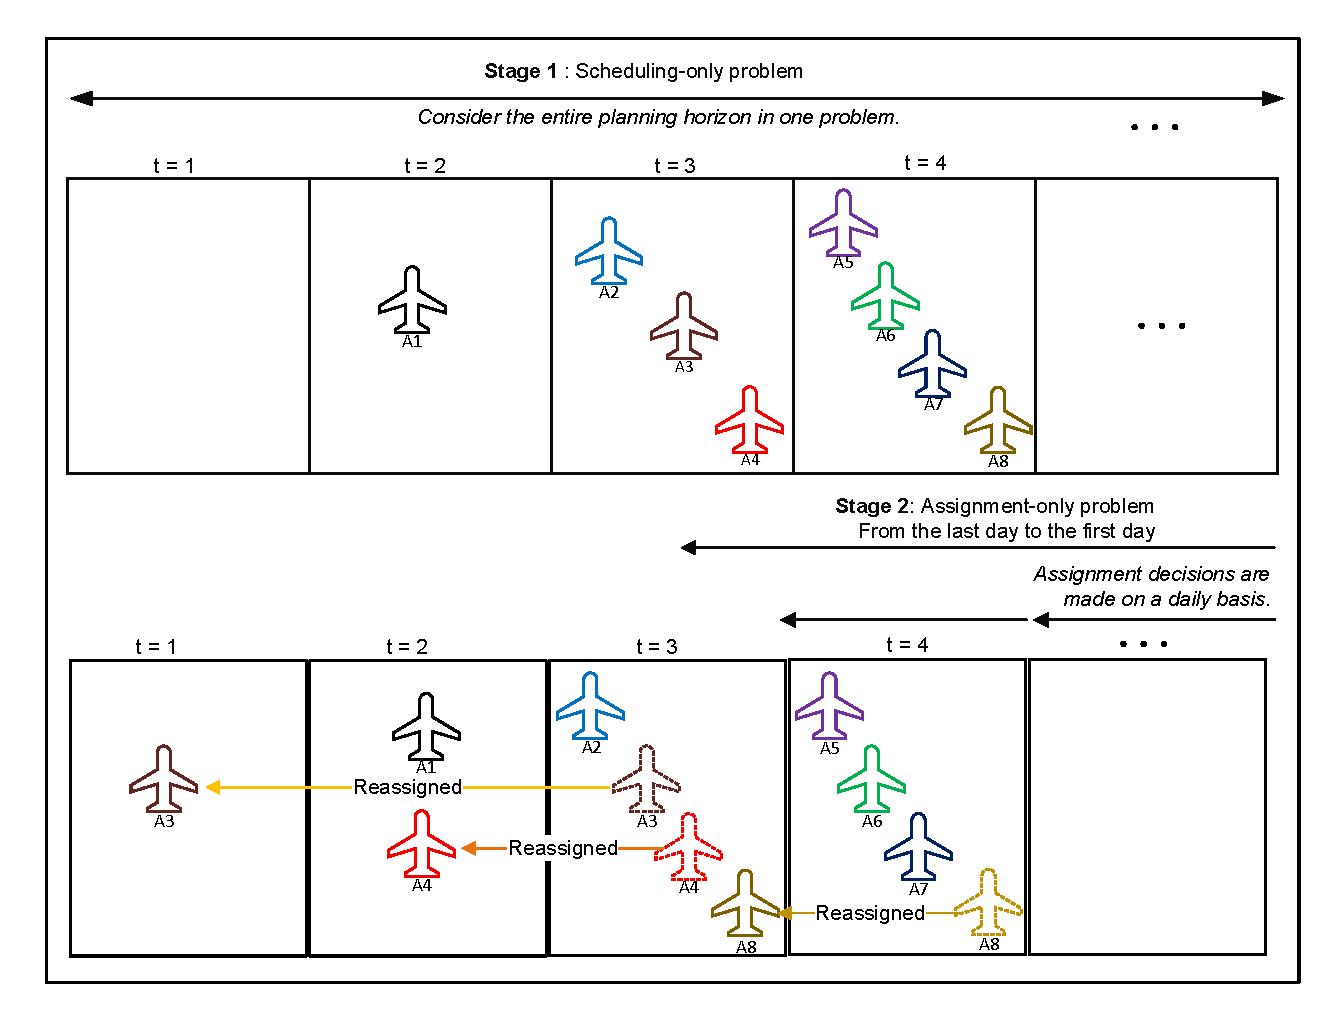
\includegraphics[width=\linewidth]{sequential_heurisicsv3.pdf}
    \caption{Illustration for the sequential heuristic decomposition framework}
    \label{fig:sh-framework}
\end{figure}


For the planning horizon $T$ in the SOP, we solve the assignment-only problem (AOP) daily, starting from the end of the planning horizon, namely Day $|T|$, going backward to the first day, namely Day 1 as shown in Figure~\ref{fig:sh-framework}. Note that not all tuples scheduled for day $t$ can be accommodated. For instance, two A checks are scheduled for a day and the total capacity is sufficient. When those two checks are assigned to two stations, infeasibility arises because one station has sufficient man hours while its station access is zero; the other station has sufficient station access while not having enough man hours. Therefore, it is likely that the aggregated capacity is sufficient while the capacity at the station level is insufficient. When such an infeasibility issue arises, namely, a tuple cannot be accommodated on a scheduled day $t$, we shift it to an earlier day $t-1$. Shifting a scheduled tuple to an earlier date will not cause the DTG to be inadmissible (i.e., dropping below the minimum value of 1).


% \begin{figure}[htbp]
%     \centering
%     \includegraphics[width=\linewidth]{sequential_heurisics.pdf}
%     \caption{Illustration for the sequential heuristic decomposition framework}
%     \label{fig:sh-framework}
% \end{figure}




\begin{table}[ht]
\centering
\caption{Notation used in the AOP}
\label{tab:notation_tabDecomp2}
\begin{tabular}{lp{16cm}} 
\toprule
\multicolumn{2}{l}{\textit{Sets and Indices}} \\ 
\hline
$I^t$ & Set of aircraft routed for maintenance on day $t$ \\
$I_s^t$ & Set of aircraft of a particular subfleet type $s$ routed for maintenance on day $t$, $I_s^t = I_s \cap I^t$ \\
$W^t$ & Set of tuples scheduled for day $t$ \\
$W_i^t$ & Set of tuples scheduled for day $t$ for aircraft $i \in I^t$ \\
$\bar{W^t}$ & Set of A check tuples scheduled for day $t$, $\bar{W^t} \subseteq W^t$ \\
$\hat{W^t}$ & Set of One-C-check tuples scheduled for day $t$, $\hat{W^t} \subseteq W^t$ \\
$\hat{W_i^t}$ & Set of One-C-check tuples scheduled for day $t$ and aircraft $i$, $\hat{W_i^t} \subseteq W^t $ \\
$\breve{W^t}$ & Set of Two-C-check tuples scheduled for day $t$, $\breve{W^t} \subseteq W^t$ \\
$\breve{W_i^t}$ & Set of Two-C-check tuples scheduled for day $t$ and aircraft $i$, $\breve{W_i^t} \subseteq W^t$ \\ 
\hline
\multicolumn{2}{l}{\textit{Parameter}}  \\
\hline
$\phi_{ij}^t$ & A binary parameter indicating whether aircraft $i$ has been routed to station $j$ for maintenance in $\eta + 1$ days from day $t$ \\
$F$ & Penalty for not accommodating a tuple, e.g., 100  \\
\hline
\multicolumn{2}{l}{\textit{Decision Variables}} \\ 
\hline
$\alpha_{wj}^t$ & A binary variable to be 1 if tuple $w$ is assigned to station $j$ for maintenance on day $t$ \\
$\theta_{ij}^t$ & A binary variable to be 1 if aircraft $i$ is routed to station $j$ for maintenance on day $t$ \\
$\hat{\varphi_j}^t$ & A binary variable to be 1 if station $j$ is open for One-C Phase checks on day $t$ \\
$\breve{\varphi_j}^t$ & A binary variable to be 1 if station $j$ is open for Two-C Phase check on day $t$  \\
$\lambda_{w}^t$ & A binary variable to be 1  if a scheduled tuple $w$ is not accommodated on day $t$ \\ 
\hline
\end{tabular}
\end{table}



Hence, with additional notation in Table~\ref{tab:notation_tabDecomp2}, we present the aircraft-to-station assignment-only problem for a given day $t$ as follows:
\begin{flalign}
\text{(AOP)} \quad \min_{\left\{\alpha_{wj}^t, \theta_{ij}^t, \hat{\varphi_j}^t,\breve{\varphi_j}^t, \lambda_{w}^t\right\}} \quad & \sum_{w \in W^t} \sum_{j \in J_w} \beta_{wj} \alpha_{wj}^t + F\sum_{w \in W^t} \lambda_{w}^t\label{eq:ObjAssignment} \\
    \text{s.t.} \quad & \sum_{j \in J_w} \alpha_{wj}^t + \lambda_{w}^t  = 1, \quad \forall w \in W^t  \label{eq:OneStationPerTuple} \\
    & \sum_{w \in W_i^t} \alpha_{wj}^t \leq M \theta_{ij}^t, \quad  \forall i \in I^t, j \in J \label{eq:LinkVisit} \\
    & \sum_{i \in I_s^t} \theta_{ij}^t   \leq  P_{sj}^t, \quad \forall s \in S,j \in J \label{eq:stationaccess_subAssin}\\
    & \sum_{w \in W^t} l_w \alpha_{wj}^t \leq H_j, \quad \forall j \in J \label{eq:StationManhours} \\
    & \sum_{i \in I^t}  \theta_{ij}^t \leq Q_j, \quad \forall j \in J\label{eq:StationCap} \\
    & \sum_{j \in J_i} \theta_{ij}^t \leq 1, \quad \forall i \in I^t \label{eq:OneStationPerAircraft} \\
    & \sum_{w \in \bar{W^t}} \alpha_{wj}^t \leq A_j^t, \quad \forall j \in J \label{eq:StationACheckCapacity} \\
    & \hat{\varphi_j^t} + \breve{\varphi_j^t} \leq 1,  \quad \forall j \in J \label{eq:sub-notsamephasechecktype} \\
    & \sum_{w \in \hat{W^t}} \alpha_{wj}^t \leq U_j^t\hat{\varphi_j^t}, \quad \forall j \in J \label{eq:sub-notsamephasechecktypehat} \\
    & \sum_{w \in \breve{W^t}} \alpha_{wj}^t \leq U_j^t \breve{\varphi_j^t}, \quad \forall j \in J \label{eq:sub-notsamephasechecktypebreve}  \\
    & \sum_{w \in \hat{W_i^t}} \alpha_{wj}^t + \sum_{w \in \breve{W_i^t}} \alpha_{wj}^t \leq R_j^t, \quad \forall i \in I^t, \forall j \in J \label{eq:PhaseCheckPerAircraft} \\
    & \phi_{ij}^t + \theta_{ij}^t \leq 1, \quad \forall i \in I^t, j \in J \label{eq:NoRepeatVisits} \\
    & \alpha_{wj}^t \in \{0,1\}, \quad \forall w \in W^t,  j \in J_w \label{eq:BinaryAssignment} \\
    & \theta_{ij}^t \in \{0,1\}, \quad \forall i \in I^t, j \in J_i \label{eq:AircraftAssignment} \\
    & \hat{\varphi_j^t} \in \{0,1\}, \quad \forall j \in J \label{eq:openOneC} \\
    & \breve{\varphi_j^t} \in \{0,1\}, \quad \forall j \in J \label{eq:openTwoC} \\
    & \lambda_w^t \in \{0,1\}, \quad \forall w \in W^t\label{eq:notassignedtuple}
\end{flalign}

The objective function Eq.~\eqref{eq:ObjAssignment} prioritizes the assignment of tuples to their preferred stations while simultaneously minimizing the total number of tuples that cannot be accommodated on day $t$.
Constraint~\eqref{eq:OneStationPerTuple} ensures that each tuple $w \in W^t$ must be scheduled for maintenance (i.e., $\sum_{j \in J_w} \alpha_{wj}^t = 1$); otherwise, $\lambda_{w}^t = 1$, meaning that tuple $w$ is left unscheduled.  
Constraint~\eqref{eq:LinkVisit} ensures that none of aircraft $i$'s check tuples can be assigned to station $j$ unless aircraft $i$ is routed to station $j$.
Constraint~\eqref{eq:stationaccess_subAssin} is the station access constraint for station $j$.
Constraint~\eqref{eq:StationManhours} is the man-hour constraint.
Constraint~\eqref{eq:StationCap} ensures that the maximum number of aircraft routed to station $j$ is capped at $Q_j$.
Constraint~\eqref{eq:OneStationPerAircraft} ensures that aircraft $i$ must be routed to a compatible station for maintenance.
Constraint~\eqref{eq:StationACheckCapacity} ensures that the number of A-check-tuples assigned to station $j$ does not exceed $A_j^t$. 
Constraint~\eqref{eq:sub-notsamephasechecktype} ensures that at station $j$, we can have only type of One-C phase checks or Two-C phase checks.
Constraint~\eqref{eq:sub-notsamephasechecktypehat} ensures that if station $j$ is open for One-C phase check, then the total number of One-C phase checks assigned to it should not exceed limit $U_j^t$.
Similarly, constraint~\eqref{eq:sub-notsamephasechecktypebreve} enforces the exact requirement but for Two-C checks. 
Constraint~\eqref{eq:PhaseCheckPerAircraft} states that the total number of phase checks performed on aircraft $i$ at station $j$ does not exceed $R_j$.
Constraint~\eqref{eq:NoRepeatVisits} ensures that when an aircraft cannot visit the same station for maintenance within a period of $\eta$ days.
Constraints~\eqref{eq:BinaryAssignment}, \eqref{eq:AircraftAssignment}, \eqref{eq:openOneC},  \eqref{eq:openTwoC}, and \eqref{eq:notassignedtuple} define decision variables as binary.



\subsection{Temporal Decomposition (TD) Approach}
\label{sec:tempDecomp}
In Section~\ref{sec:SchedulingThenAssign}, the overall strategy is to decompose the optimization problem based on the type of decisions (scheduling vs assignment). We next present a different decomposition strategy, which is based on time. The temporal decomposition can be described with a rolling horizon framework, illustrated in Figure~\ref{fig:temp-dec_illustration}. 

\begin{figure}[htbp]
    \centering
    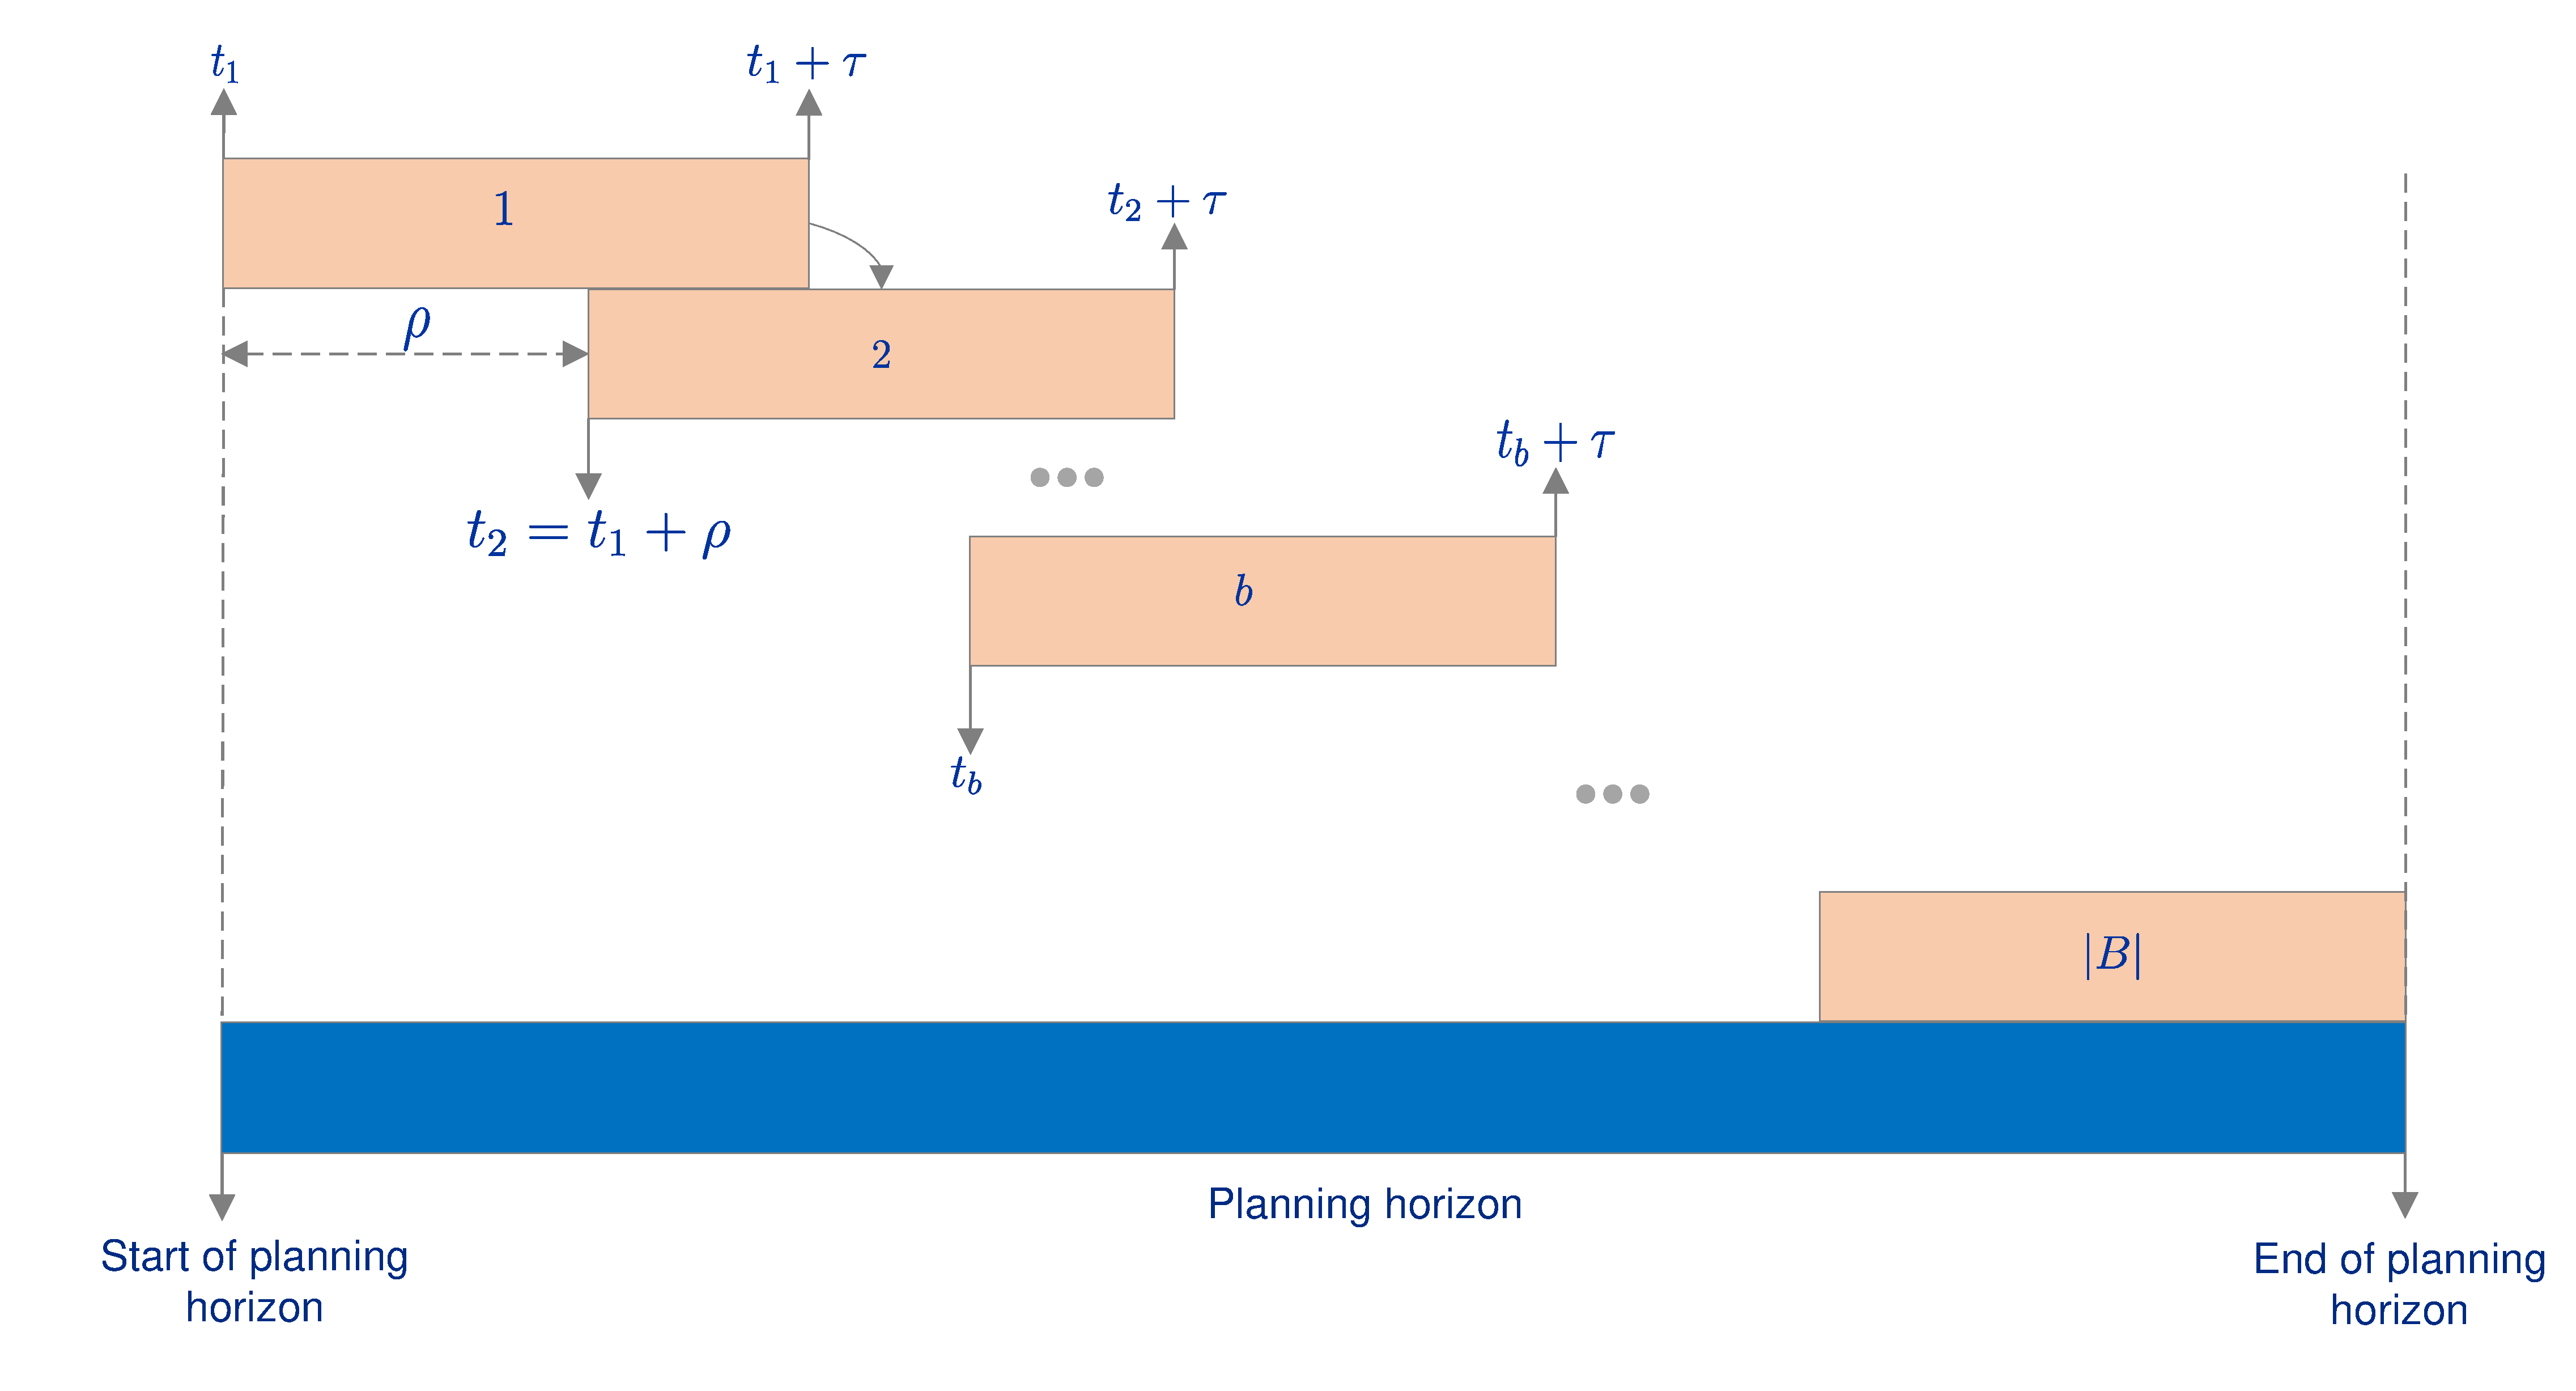
\includegraphics[width=\linewidth]{updated_temporal_decompositionv2.pdf}
    \caption{Illustration for the temporal decomposition framework}
    \label{fig:temp-dec_illustration}
\end{figure}



The original planning horizon $T$ is decomposed into a series of partially overlapping time horizons of equal length $\tau$. Each time horizon $b$ begins at $t_b$ and ends at $t_b + \tau$, where $b \in \{1, 2, \dots, |B|\}$ and $|B|$ is the total number of time horizons. The start time of the immediate next time horizon, namely $b+1$, is $t_b + \rho$, where $\rho$ is the rolling period. As $\rho < \tau$, some overlap between time horizons $b$ and $b+1$ is built in by design. The primary motivation for keeping the overlap between two consecutive time horizons is to address the End-of-Horizon effect described in Proposition~\ref{lem:EndOfHorizon}. We can illustrate this with a simple case where the first horizon covers Day 1 to Day 10, and the second horizon covers Day 11 to Day 20. As there is no overlap between the two horizons, it is possible that for certain tuples, the DTG is 1 on Day 10, while no maintenance is scheduled on Day 10. On Day 11, the DTG would drop to zero for the above said tuples, thus leading to infeasibility issues. 

We next describe how a joint optimization problem $\Delta_b$ is formulated for time horizon $b$. Among all those tuples in $W$, only those tuples meeting $\delta_w^0 \leq t_b + \tau + \epsilon$ are considered in $\Delta_b$, where $\delta_w^0$ is the updated DTG for each tuple $w \in W$ at $t_b$. The formulation Eqs.~\eqref{eq:ObjDaystogo} to \eqref{eq:JointBinary4} is built based on the above stated subset of $W$ and a planning horizon of $t_b$ to $t_b + \tau$. After solving problem $\Delta_b$, we obtain the optimum values of key decision variables, such as $\bar{x}_{wj}^t$, $\bar{y}_w^t$, and $\bar{z}_{ij}^t$. Those planning decisions in the first part of time horizon $b$, namely from $t_b$ to $t_b + \rho$, are finalized; however, those planning decisions in the second part, namely from $t_b + \rho$ to $t_b + \tau$, will be re-optimized in the next time horizon $b+1$. 

With the above described approach, we solve the joint problem for each time horizon sequentially until planning decisions over the entire planning horizon are available.



For each horizon $b$, constraint~\eqref{aircraft_rotation} is defined for the following days in horizon $b$: $t_b, t_b+1,\dots,t_b+\tau-\eta+1$. Constraint~\eqref{aircraft_rotation} defined for day $t$ covers the following period of $\eta$ days: $t, t+1,\dots,t+\eta-1$. However, the aircraft rotation constraint is not enforced for the following $\eta$-day periods consisting of day $t_b$:
\begin{itemize}
    \item $t_b-\eta+1,\dots,t_b-1,t_b$
    \item $t_b-\eta+2,\dots,t_b,t_b+1$
    \item $t_b-\eta+3,\dots,t_b,t_b+2$
    \item $\dots$
    \item $t_b-1,\dots,t_b +\eta-2$
\end{itemize}

\begin{figure}[htbp]
    \centering
    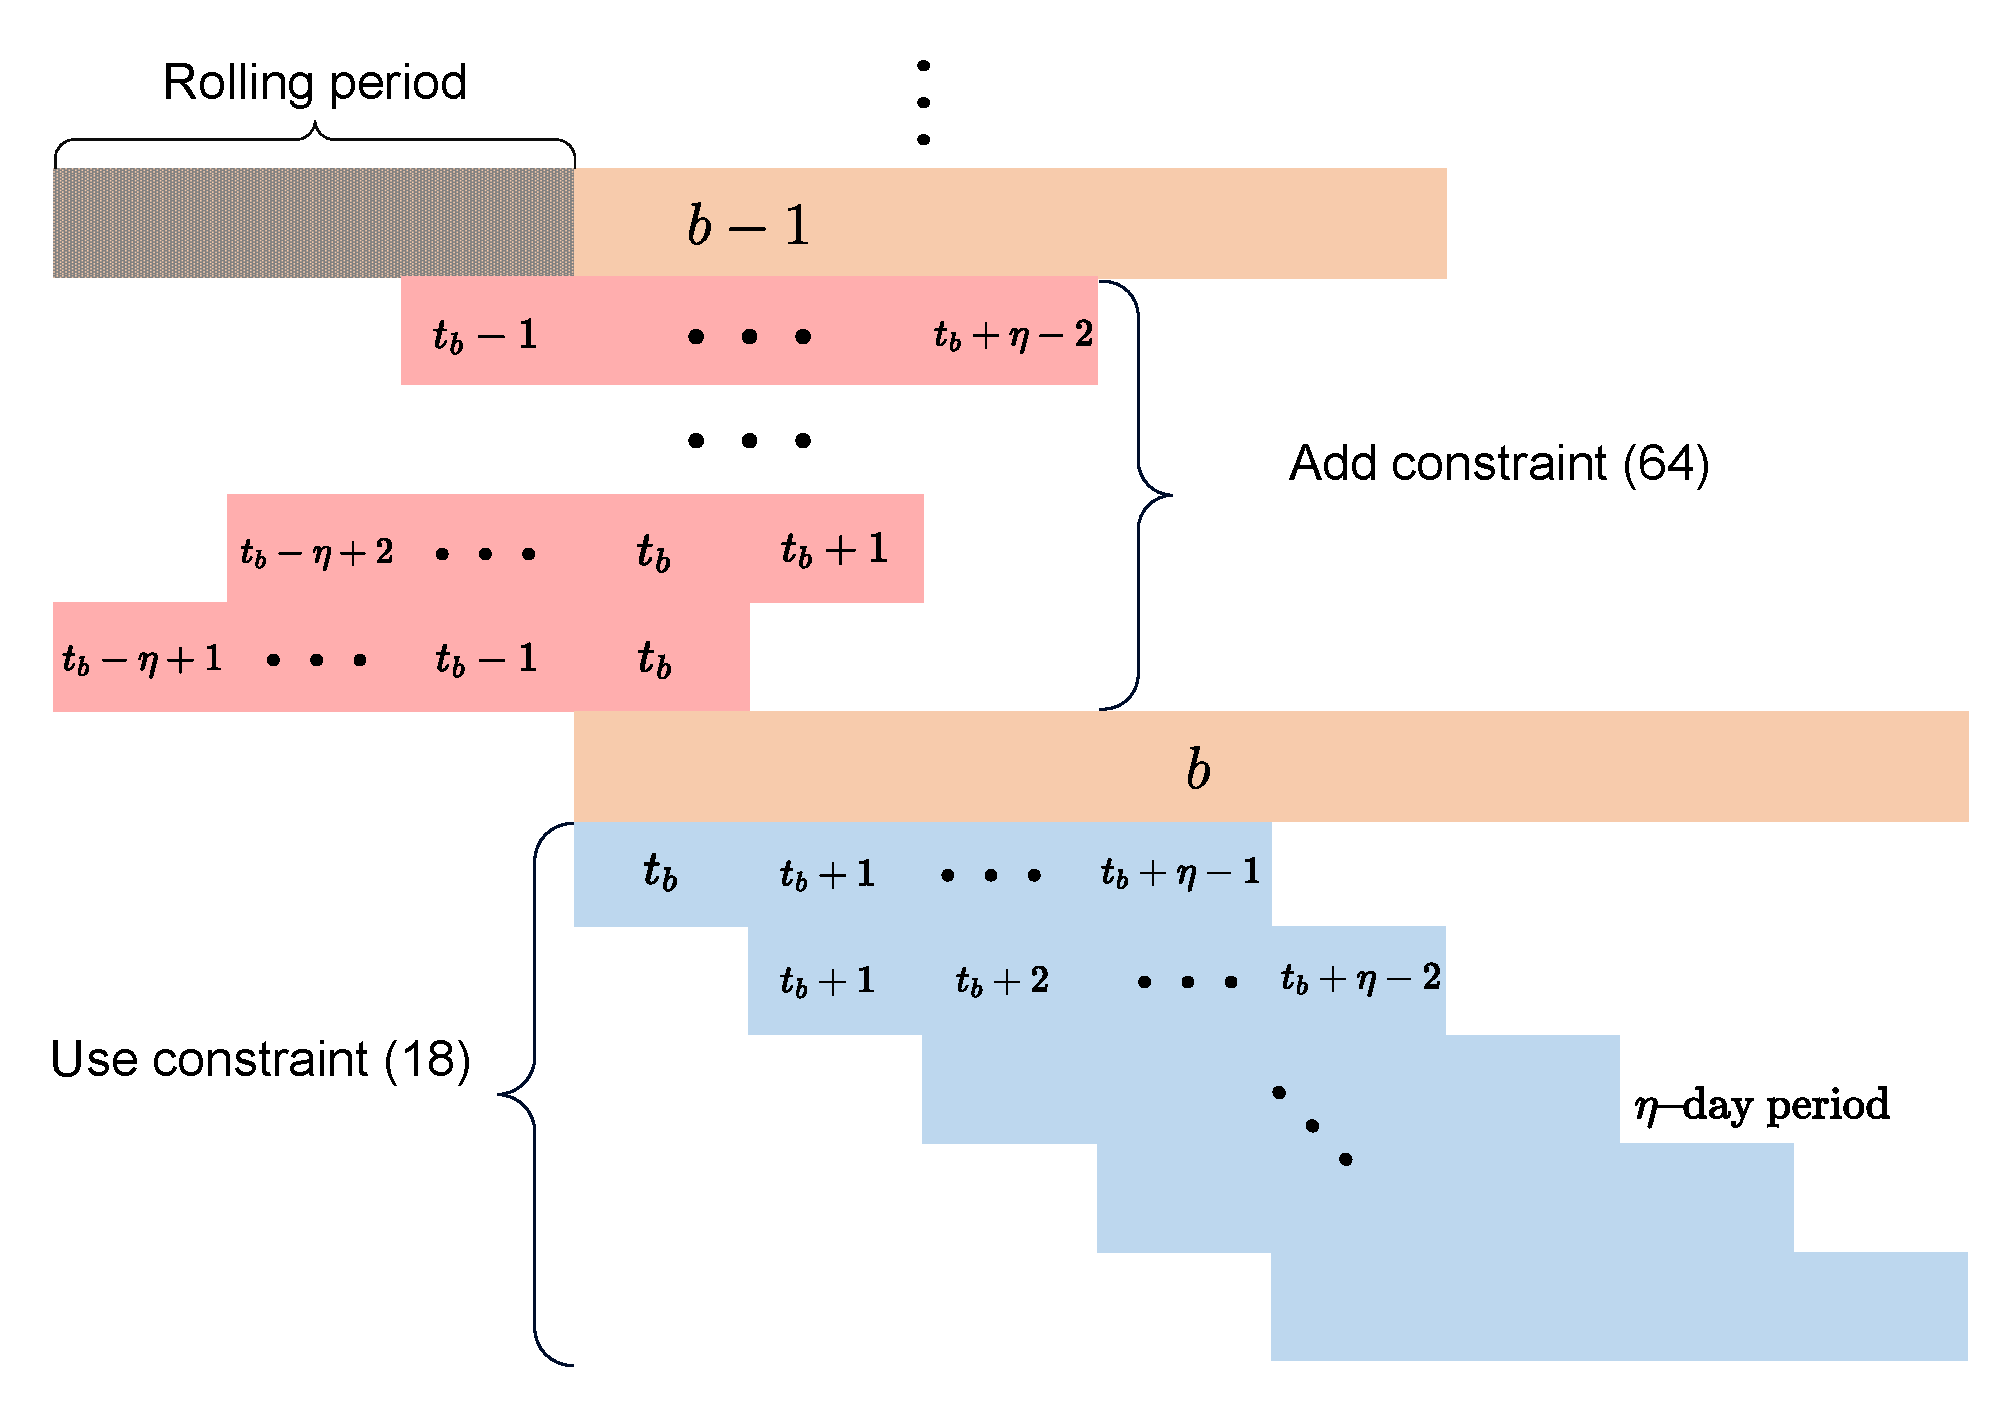
\includegraphics[width=0.7\linewidth]{rh_station_rotation_constraint.pdf} 
    \caption{Diagrammatic explanation of the constraint for aircraft rotation in the temporal decomposition}
    \label{fig:td_stat_rotate}
\end{figure}

Therefore, we add the following constraint to enforce the aircraft rotation constraint and add it to the joint problem for horizon $b$:
\begin{equation}
    \sum_{t'=t - \eta+1}^{t-1} \bar{z}_{ij}^{t'} + z_{ij}^t \leq 1, \quad \forall i \in I, j \in J, t \in \{t_b, t_b +1, \dots, t_b +\eta-2\}, \label{eq:transitionOverTb}
\end{equation}
where $\bar{z}_{ij}^{t'}$ are optimized decisions from the previous horizon, namely horizon $b-1$, and considered as given when solving the problem for horizon $b$.


The effectiveness of the above temporal decomposition approach depends on two key parameters, namely, time horizon $\tau$ and rolling period $\rho$. Using a shorter time horizon reduces computational time but may deteriorate the solution quality due to the limited horizon. In other words, planning is conducted locally within each horizon without considering anything outside of the subject horizon. When the rolling period $\rho$ is small (i.e., the overlap between two time horizons is large), the joint optimization problem is solved more frequently.
This increased frequency, however, results in larger total computation time. When $\rho$ is large, i.e., the overlap between two horizons is small, suboptimality or infeasibility might occur. For example, in the first horizon ranging from Day 1 to Day 10, no maintenance would be scheduled for those tuples with a DTG of 2 on Day 10. This myopic decision is made because of the anticipation that maintenance can be feasibly scheduled on Day 11 in the next horizon for those tuples. However, it might be possible that in the first few days of the second horizon, station access or another capacity parameter is insufficient to accommodate the those tuples, thus causing an infeasibility issue. Even if infeasibility can be avoided, suboptimal planning decisions occur. The likelihood of experiencing infeasibility reduces when the overlap between two horizons increases.

Given the above discussion, we perform a grid search to find the best combination of $\tau$ and $\rho$ to make a good trade-off between the objective value and the computation time. We choose $\tau$ from 20 to 30 days and $\rho$ from 10 to 15 days, with the same step size of five days. 
% Note that optimum tau and rho can differ for each problem (i.e., each problem size)









\section{Case Studies}
\label{section:case_studies}

All the data involved in this section were provided by AA for research purposes only. Due to a non-disclosure agreement, raw data are not presented while characteristics and high-level summaries of the data are provided. All of the following analyses were implemented in Python 3.12 on a personal computer (i9-13900H  Processor @ 2.60GHz and 32 GB RAM). Gurobi Optimizer (version 11.0.3) was used as the integer programming solver. 

This section is organized as follows.
Section~\ref{sec:real-world-data} describes the input data. Section~\ref{subsection:jp_result} presents results from solving the JP with a solver and Section~\ref{subsection:jp_resultReducedCap} further explores the impact of maintenance capacity reductions. Section~\ref{performance_decomp} fully examines the performance of two proposed decomposition approaches, followed by a long-term analysis in Section~\ref{sec:long_termAna} and an extension in Section~\ref{sec:twoHolidays}.

% This section is organized as follows. 
\subsection{Input Data}
\label{sec:real-world-data}

% \subsubsection{Aircraft-Check data}
The given fleet comprises over eight hundred aircraft, covering twelve subfleet types. The set of mandatory checks for each subfleet type is available. For instance, each A321E needs to complete ten different phase checks in addition to the A check. By contrast, each 738M needs to complete A checks only. As the number of checks associated with a subfleet type varies from 1 to 11, the total number of aircraft-check tuples, namely $|W|$, is over 3,100.

Each tuple $w$ has an initial DTG $\delta_w^0$ and a maximum allowable DTG, also called maintenance interval $m_w$. The interval varies significantly with the maintenance type, e.g., from around 100 days to around 700 days. For certain phase checks, the interval may go beyond 1,000 days. Each tuple also has a man-hour requirement. On average, a check requires 100 man-hours based on the provided data. 


% \subsubsection{Maintenance station data}
There are in total 15 maintenance stations with different capabilities and capacity specifications. Each station is capable of serving certain subfleet types or certain checks of a subfleet type. Therefore, each station is associated with a subset of tuples it can service. Additionally, each station $j$ has the following specifications: man-hours available $H_j$, the maximum number of A checks that station $j$ can handle $A_j$, the maximum number of phase checks that can be performed $U_j$, the number of distinct aircraft $Q_j$ that station $j$ can handle daily, and the maximum number of phase checks that can be performed simultaneously on a given aircraft at station $j$, i.e., $R_j$. Most stations can accommodate one aircraft for maintenance daily, while some stations can accommodate two. In other words, $Q_j$ is mostly 1. $A_j$ is 1 for all stations. As some stations cannot handle phase checks, $U_j$ can be 0, 1, or 2. For those stations with a positive $U_j$, $R_j$ is either 1 or 2. Note that when the above capacity parameters vary over time, a superscript $t$ is added to obtain $H_j^t$ from $H_j$, for instance.


In this long-term problem, the flight schedule information is available in the form of station access, which specifies on each day how many aircraft of a subfleet type can be routed to a station for maintenance. The station access data are from the fleet assignment process, which occurs a few months in advance. The station access varies significantly, ranging from 0 to over 50. In most cases, $P_{sj}^t$ is quite small, e.g., less than four if not zero.


The planning horizon $T$ ranges from April 16 to October 12, 2024, which covers 180 days. For some tuples that are due for maintenance in the first week of the planning horizon, their scheduled maintenance dates have been given by the aircraft maintenance routing team and cannot be modified. Those tuples are also referred to as pre-scheduled tuples. Due to the consideration of such pre-scheduled tuples, the remaining capacity of a maintenance station varies over time.

The baseline values of other parameters are specified as follows: $\gamma = 0.99$; $\eta = 3$; $\epsilon = 15$; $\beta_{wj}$ varies from 0.9 to 1. A lower value of $\beta_{wj}$ represents more preference of tuple $w$ for station $j$.
% The value of $\eta$  is 3.

\subsection{Joint Problem Optimization Results under Full Capacity}
\label{subsection:jp_result}

We first solve an instance with a 60-day planning horizon (i.e., $|T| = 60$) from April 16, 2024 to June 14, 2024. After pre-processing (i.e., dropping those tuples with an initial DTG greater than $|T| + \epsilon$), there are 377 aircraft and 567 tuples for scheduling and assignment. Among 567 tuples, 11 tuples have been prescheduled over the first week by the aircraft maintenance routing team at AA. After solving the joint optimization problem, 408 tuples have been scheduled over the 60-day planning horizon. Specifically, Figure~\ref{fig:60_day_planning_horizon} shows the number of scheduled tuples on each day. 
% In the first week of the planning horizon, 
The daily number of scheduled tuples varies from 1 to 17. As stated in Proposition~\ref{lem:EndOfHorizon}, no tuples are scheduled for maintenance on Day 60, the final day of the horizon. Figure~\ref{fig:60_day_planning_horizon} also shows how the man-hour utilization ratio, 
computed as $\left(\sum_{j \in J}\sum_{w \in w}l_wx_{wj}^t\right) /\sum_{j \in J}\bar{H}_j^t$, varies over time. The average man-hour utilization ratio over the entire planning horizon is only 31.5\% because all 15 stations are made available over the planning horizon in the current scenario. 


\begin{figure}[htbp]
    \centering
    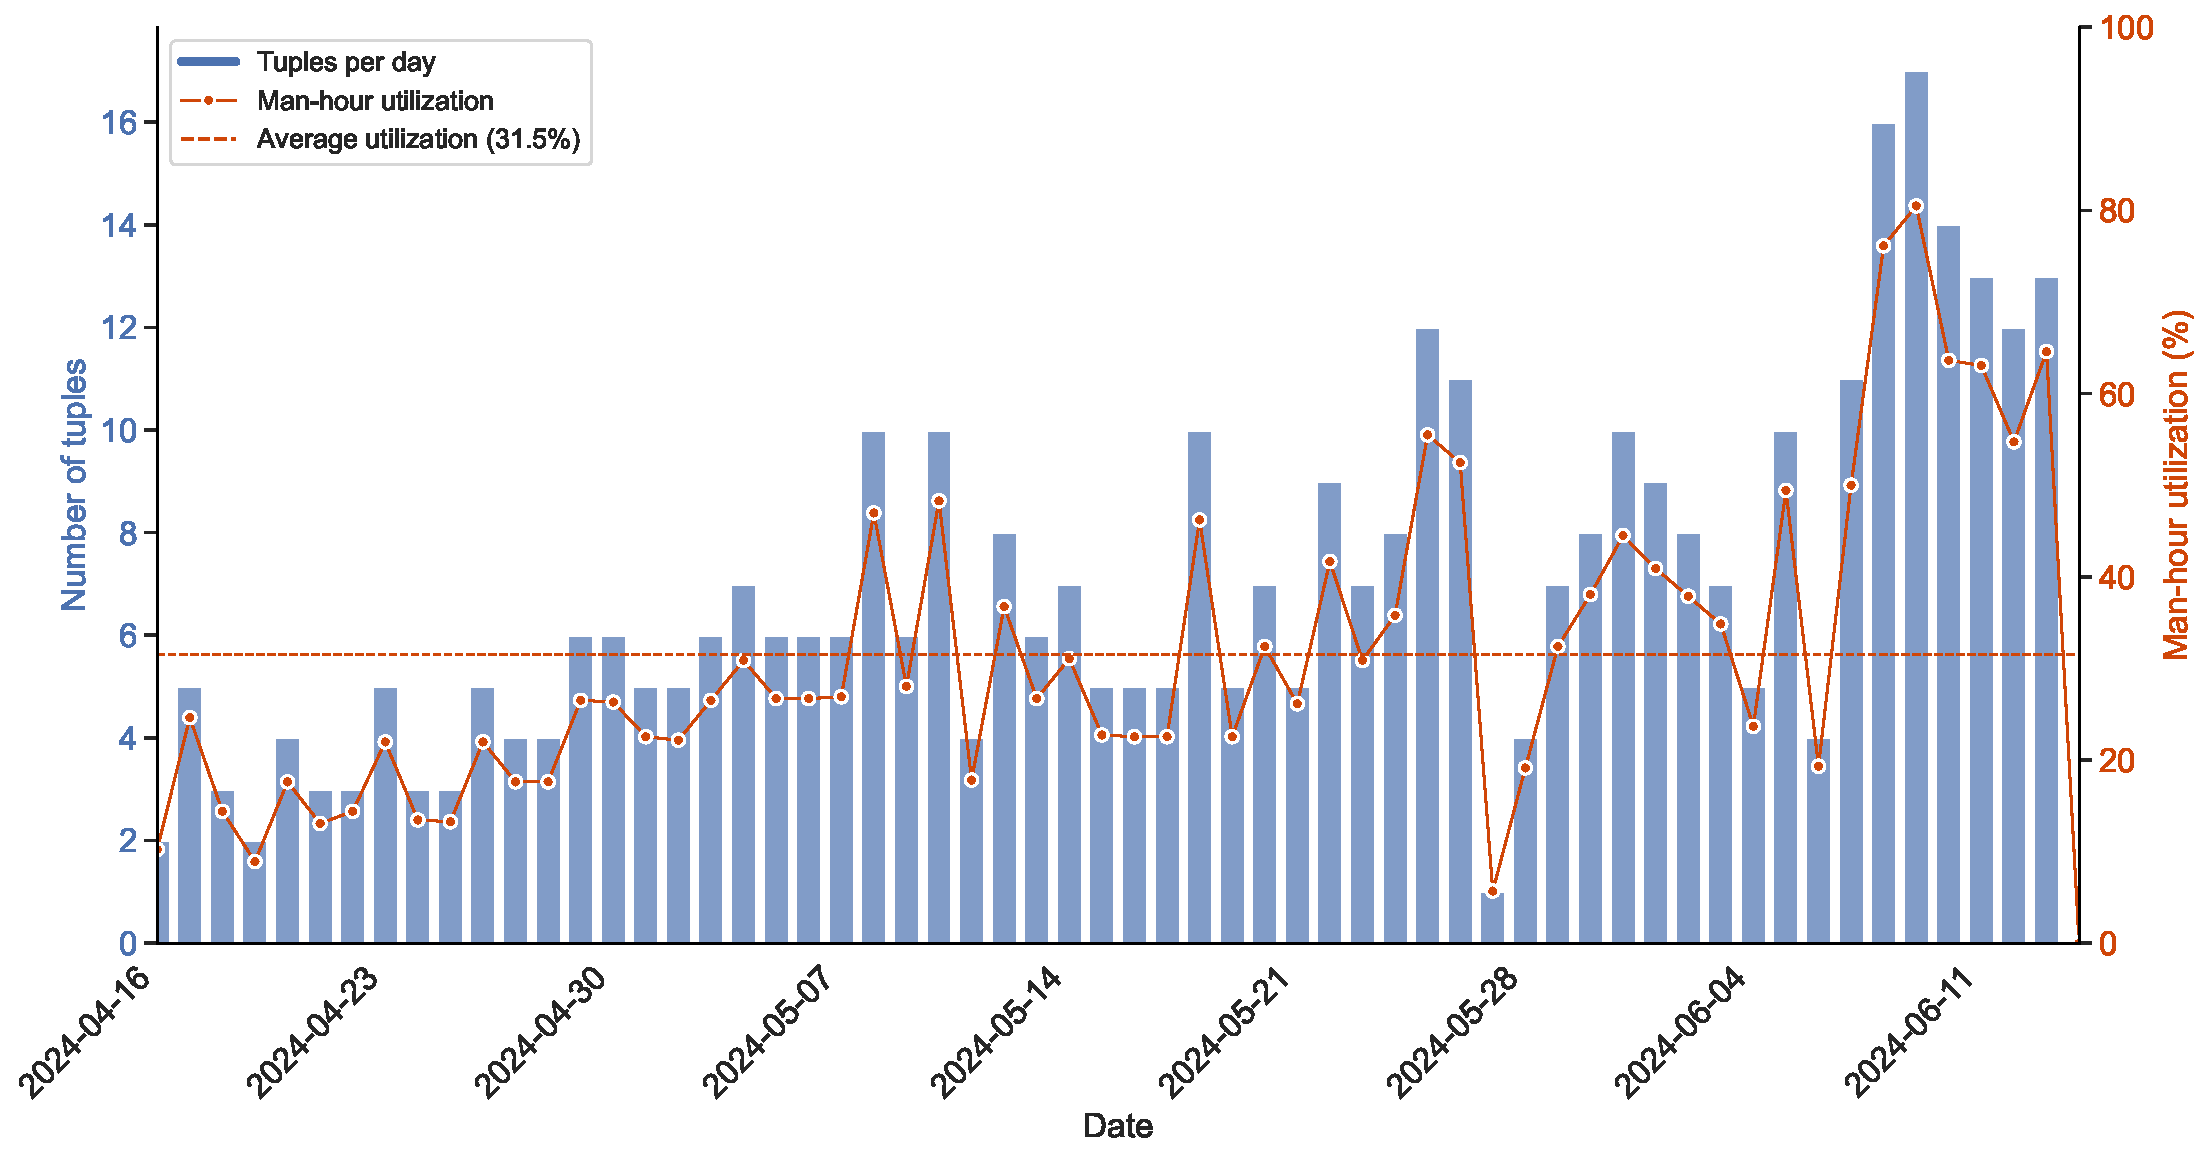
\includegraphics[width=\linewidth]{60_day_check.pdf}
    \caption{Aircraft maintenance scheduling results over a 60-day planning horizon}
    \label{fig:60_day_planning_horizon}
\end{figure}

Figure~\ref{fig:dtg_distribution} presents the distribution of the DTG on the day of maintenance for each scheduled tuple. When a tuple is scheduled for maintenance on the latest possible day, i.e., with a DTG of 1, a 100\% yield can be achieved (i.e., no useful days are wasted). It can be seen that zero waste can be achieved for 83.6\% of the scheduled tuples. Other tuples are scheduled for maintenance prematurely. In other words, a tuple is scheduled for maintenance before its due date mainly due to capacity constraints.

\begin{figure}[htbp]
    \centering
    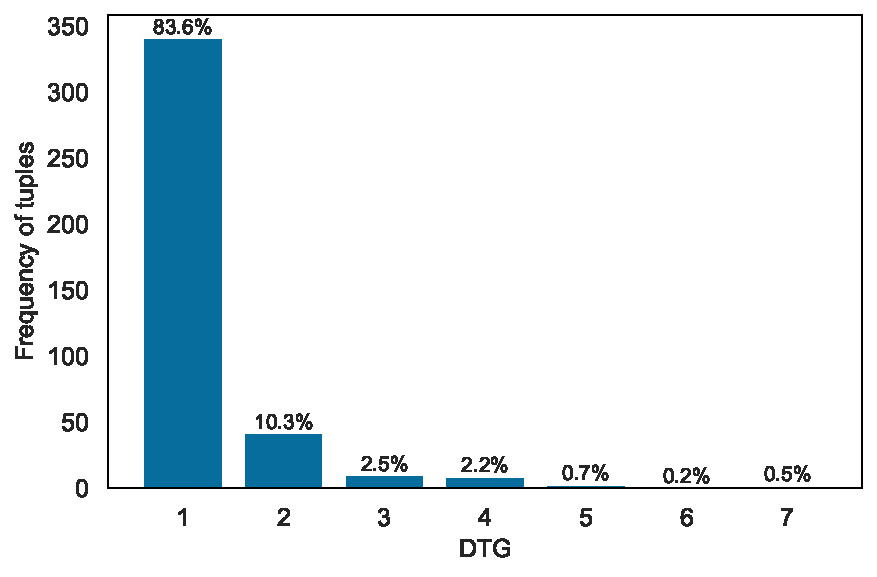
\includegraphics[width=0.6\linewidth]{dtg_hist.pdf}
    \caption{Distribution of resulting DTG on the maintenance day}
    \label{fig:dtg_distribution}
\end{figure}

Figure~\ref{fig:tuples_stat} first shows the distribution of scheduled tuples by check type. Over half of the scheduled tuples are A checks, while the rest are One-C or Two-C checks. This distribution is understandable, as A checks have a relatively short maintenance interval, and One-C checks need to be conducted more frequently than Two-C checks. Regarding C checks, we note that one or two phase checks can be scheduled for one aircraft on a day. The optimization results indicate that in 7.2\% of the cases, Two-C checks are conducted for an aircraft on the same day. Figure~\ref{fig:tuples_stat} further shows the distribution of these scheduled tuples across maintenance stations. Notably, Stations 17 and 31 accommodate a large number of A checks only without serving any phase checks due to their capabilities. The number of scheduled tuples per station ranges from less than 10 to over 50.


\begin{figure}[htbp]
    \centering    
    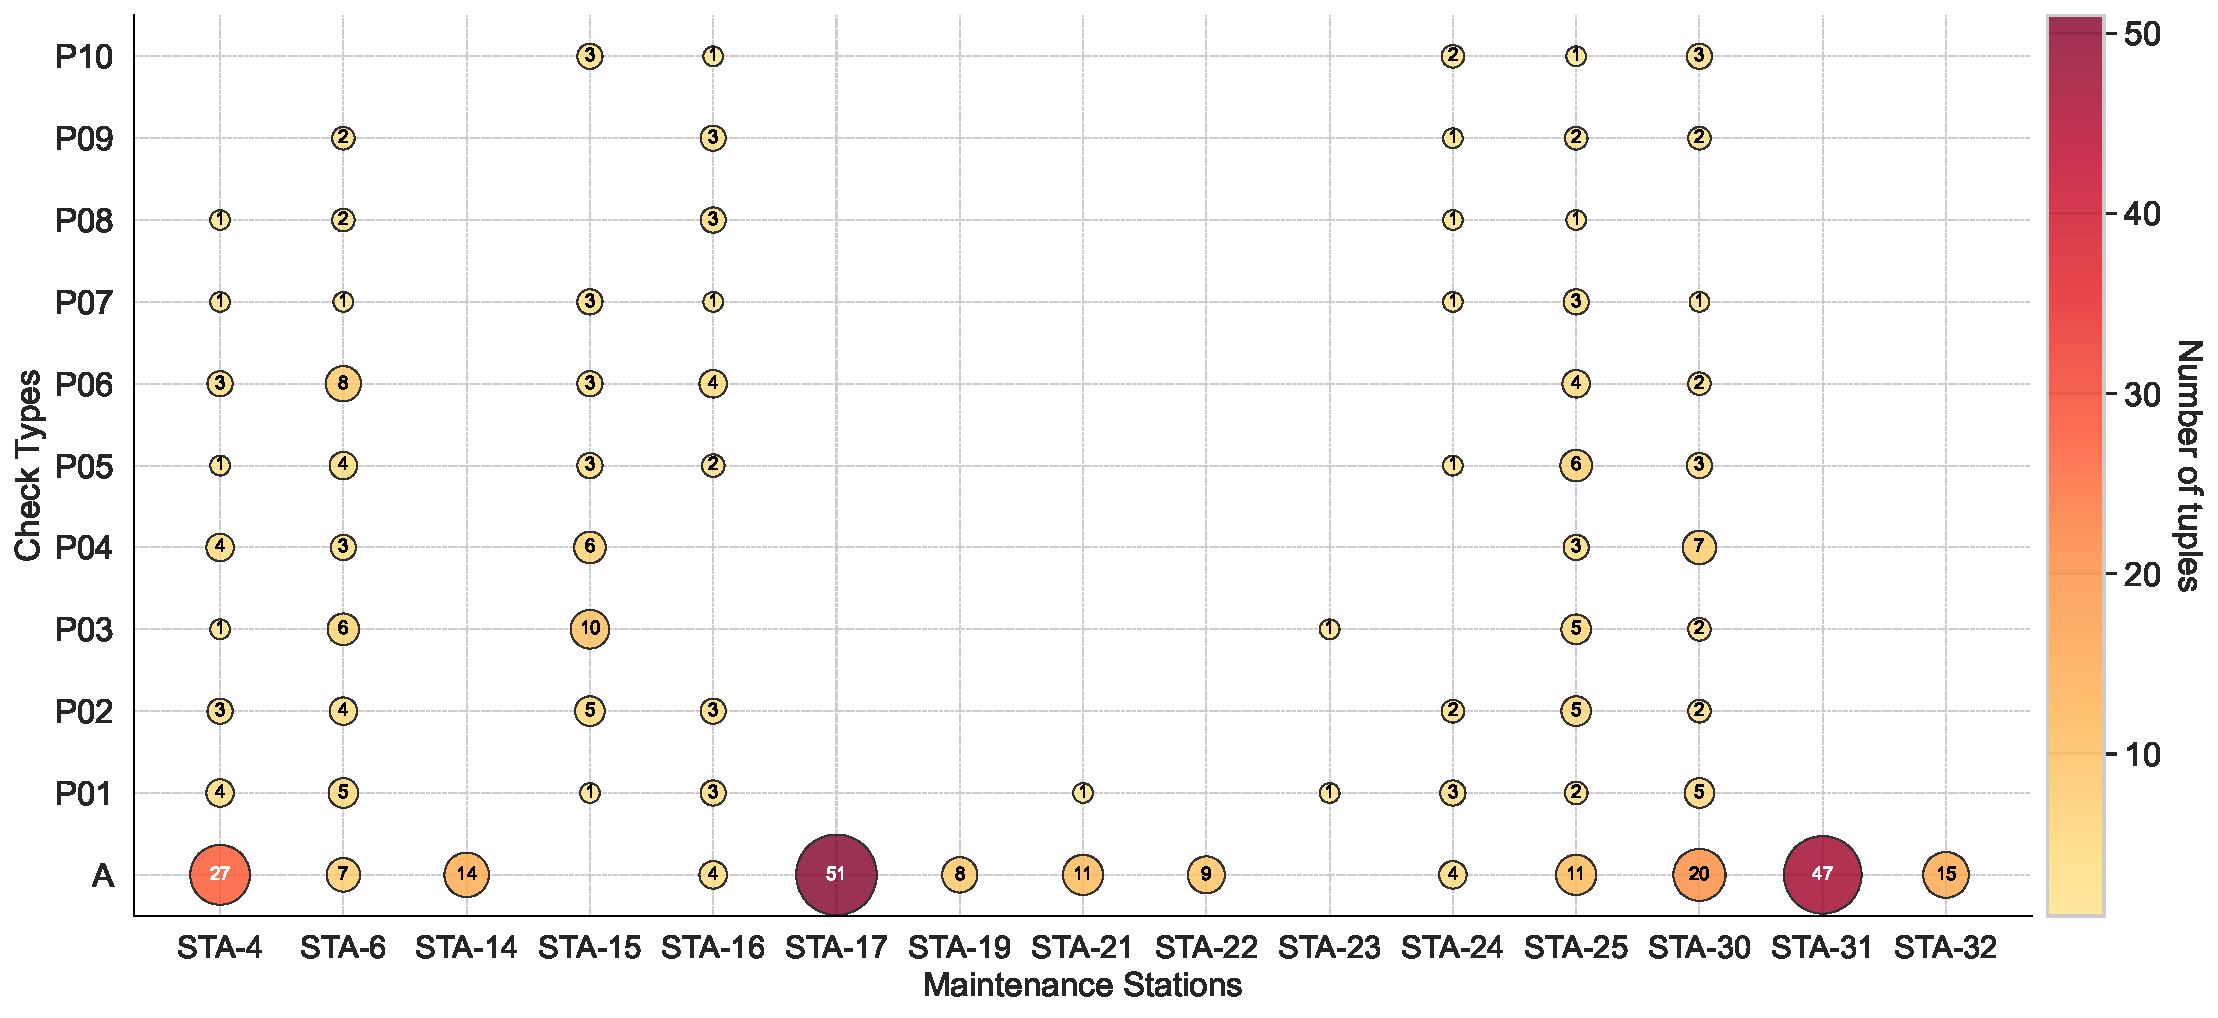
\includegraphics[width=\linewidth]{check_a_sta.pdf}
    \caption{Distribution of scheduled checks over check types and maintenance stations}
    \label{fig:tuples_stat}
\end{figure}


After analyzing the optimization results, we examine the computation time. For the 60-day planning horizon, the total computation time is 421 seconds. We next increase the planning horizon length and observe how the computation time increases accordingly in Table~\ref{tab:increase_tuple}. Note that a longer planning horizon also implies more tuples for planning, as well as more variables and constraints. It can be observed that as the planning horizons $|T|$ increase, the solution time increases exponentially. For the 100-day planning horizon, we could not achieve an optimal solution within the time limit of 7,200 seconds, although the final optimality gap is 0.76\%, provided by the solver. Note that when $|T| = 100$, the resulting integer program has over three million constraints and one million variables.




\begin{table}[htbp]
\centering
\caption{Effect of planning horizon length $|T|$ on computation time}
\label{tab:increase_tuple}
\resizebox{0.8\columnwidth}{!}{%
\begin{tabular}{@{}ccccc@{}}
\toprule
\textbf{$|T|$} & Number of tuples & Number of constraints & Number of variables & Time (secs) \\ \midrule
50 & 462 & 741,248 & 371,150 & 204 \\
60 & 567 & 1,098,688 & 559,020 & 421 \\
70 & 699 & 1,569,144 & 821,240 & 782 \\
80 & 818 & 2,061,026 & 1,098,000 & 1,986 \\
90 & 934 & 2,596,364 & 1,407,780 & 3,942 \\
100 & 1053 & 3,219,916 & 1,772,000 &$>$7,200 \\ \bottomrule 
\end{tabular}%
}
\end{table}



\subsection{Joint Problem Optimization Results under Capacity Reductions}
\label{subsection:jp_resultReducedCap}
In Section~\ref{subsection:jp_result}, all 15 maintenance stations are available. We next explore how optimization results would differ when some stations are unavailable. Each of the 15 stations can accommodate one A check daily while the number of phase checks $U_j$ differs. Depending on how many phase checks a station can accommodate daily, we divide 15 stations into three categories: (i) six stations cannot accommodate any phase checks ($U_j = 0$); (ii) seven stations can accommodate one phase check daily ($U_j = 1$); and (iii) two stations can accommodate two phase checks daily ($U_j = 2$). We then design the following capacity reduction scenarios, shown in Table \ref{tab:capacity_reduction}. In each scenario, the number of stations is reported by category, along with the capacity limits.

\begin{table}[htbp]
\centering
\caption{Capacity reduction scenarios}
\label{tab:capacity_reduction}
\resizebox{\columnwidth}{!}{%
\begin{tabular}{@{}cccccccc@{}}
\toprule
Scenario & Category (i) & Category (ii) & Category (iii) & Total \# of stations & A check limit & Phase check limit & MH limit \\ \midrule
1 & 6 & 7 & 2 & 15 & 15 & 11 & 2,112 \\
2 & 5 & 5 & 2 & 12 & 12 & 9 & 1,704 \\
3 & 4 & 4 & 2 & 10 & 10 & 8 & 1,464 \\
4 & 4 & 4 & 1 & 9 & 9 & 6 & 1,224 \\
5 & 3 & 3 & 1 & 7 & 7 & 5 & 984
\\ \bottomrule
\end{tabular}%
}
\end{table}


 

\begin{figure}[htbp]
    \centering
     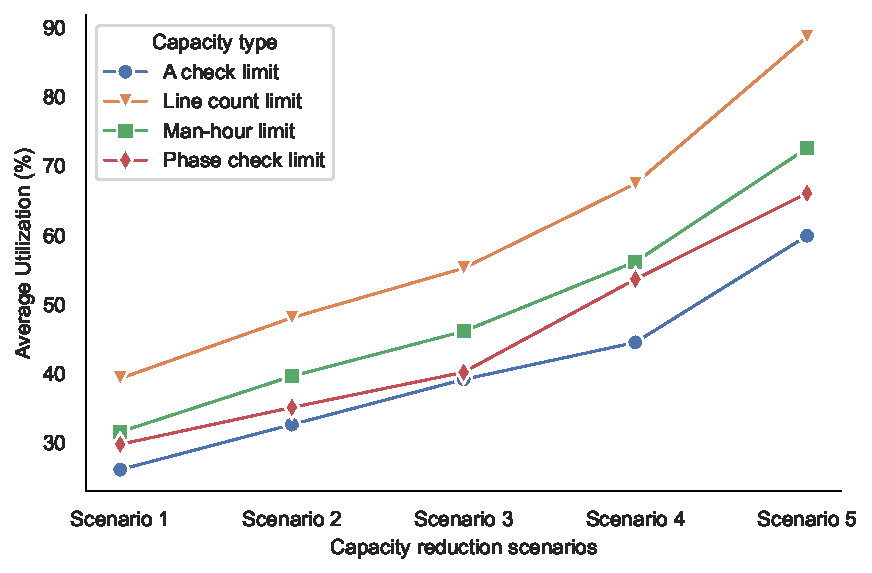
\includegraphics[width=0.7\linewidth]{utilization_v1.pdf}
    \caption{Capacity utilization ratios under different scenarios}
    \label{fig:impact_utilization}
\end{figure}

We resolve the joint problem under each capacity reduction scenario using the same 60-day planning period. Instead of presenting detailed optimization results under each scenario, Figure~\ref{fig:impact_utilization} shows the average capacity utilization over all applicable stations and over time for each capacity type. The A check capacity utilization ratio is calculated as $\left(\sum_{j \in J}\sum_{w \in \bar{W}}x_{wj}^t\right) /\sum_{j \in J}\bar{A}_j^t$. Similarly, the phase check capacity utilization ratio is $\left(\sum_{j \in J}\sum_{w \in \hat{W}\cup\breve{W}}x_{wj}^t\right) /\sum_{j \in J}\bar{U}_j^t$ and the line count utilization ratio is $\left(\sum_{j \in J}\sum_{i \in I}z_{ij}^t\right) /\sum_{j \in J}\bar{Q}_j^t$. It is clear that as the number of available stations drops, i.e., the amount of available capacity drops, the capacity utilization for each capacity type increases consequentially, since the maintenance demand is fixed. Notably, the line count (the number of distinct aircraft a station can handle) has the highest average utilization, which is nearly 90\% in Scenario 5.

Understandably, for the same maintenance demand, reducing the number of available maintenance stations leads to premature maintenance due to an increasing likelihood of having binding capacity constraints. 


\begin{figure}
    \centering
    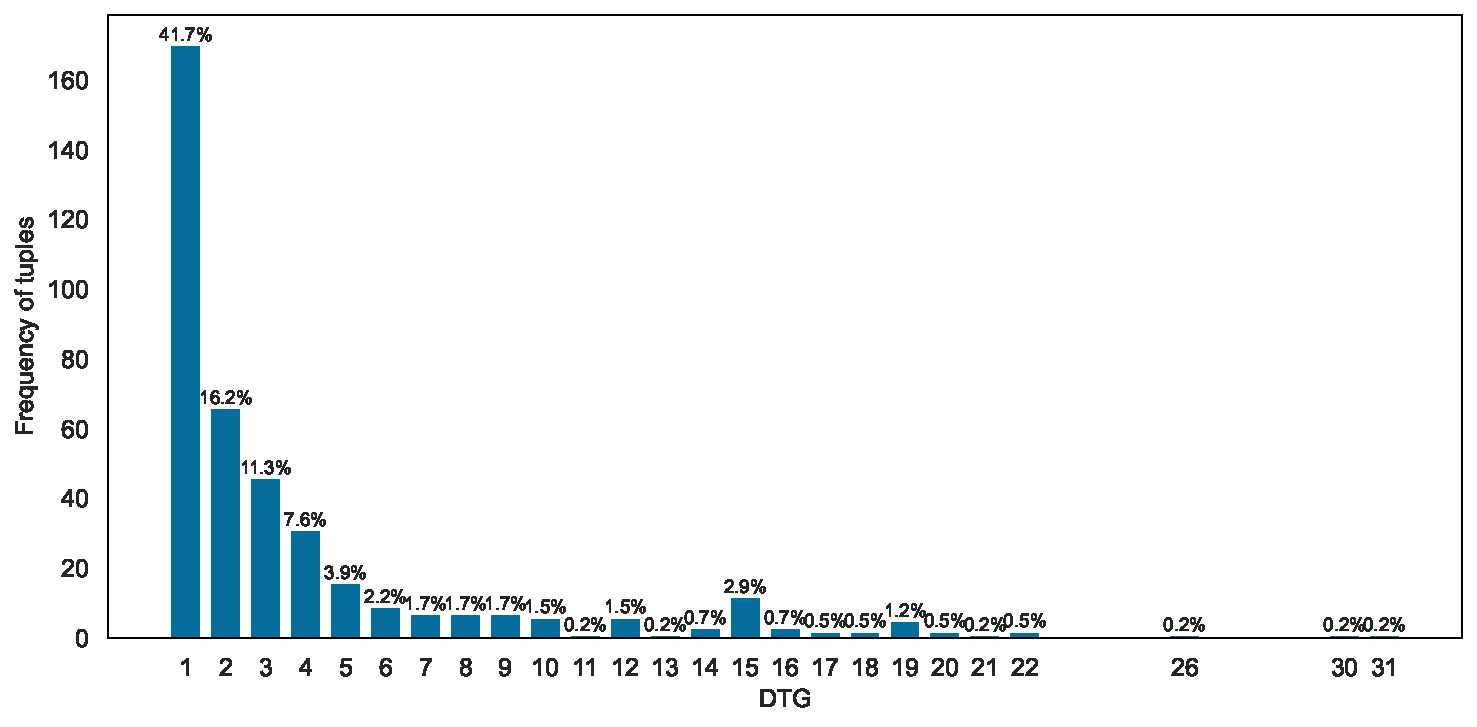
\includegraphics[width=\linewidth]{dtg_hist_s5.pdf}
    \caption{Distribution of resulting DTG on the maintenance day under Scenario 5}
    \label{fig:scenario5DTG}
\end{figure}

Figure~\ref{fig:scenario5DTG} shows the resulting distribution of DTGs on the day of maintenance under Scenario 5. As compared with Figure~\ref{fig:dtg_distribution}, fewer tuples can achieve a 100\% yield (i.e., zero waste) when the capacity is substantially reduced. We also note that reducing the number of maintenance stations results into a higher optimization objective (discounted maintenance cost).



\begin{table}[htbp]
\centering
\caption{Effect of capacity reductions on computation time }
\label{tab:my-cap-reduction-time}
\resizebox{0.8\columnwidth}{!}{%
\begin{tabular}{@{}ccccc@{}}
\toprule
\multicolumn{1}{l}{Scenario} & Number of stations & Number of constraints & Number of variables & Time (secs) \\ \midrule
1 & 15 & 1,098,688 & 559,020 & \textbf{421} \\
2 & 12 & 917,848 & 447,540 & 431 \\
3 & 10 & 795,328 & 361,860 & 495 \\
4 & 9 & 740,488 & 331,860 & 513 \\
5 & 7 & 640,168 & 301,740 & 6,086 \\ \bottomrule
\end{tabular}%
}
\end{table}


Table~\ref{tab:my-cap-reduction-time} shows that as the number of available stations decreases, the computation time increases. Note that the computation time of 421 seconds under the full-capacity scenario is reported earlier in Table~\ref{tab:increase_tuple}. Hence, with fewer stations, the joint optimization becomes more constrained with limiting flexibility in scheduling and assignment decisions.  Although the numbers of variables and constraints reduce, it is increasingly difficult to find feasible planning decisions due to increasingly tight capacity constraints, which indirectly leads to increased computational time. 

\subsection{Performance of Decomposition-Based Solution Approaches}
\label{performance_decomp}


Section~\ref{subsection:jp_result} has demonstrated that directly solving the JP (i.e., benchmark approach) is impractical when $|T|$ is large. Section~\ref{subsection:jp_resultReducedCap} further shows that the computation time also increases dramatically when few maintenance stations are available. As no other studies have addressed the joint scheduling and station assignment decisions, we cannot compare the two decomposition-based solution approaches with any existing algorithms. Instead, both proposed solution approaches are benchmarked with directly solving the JP with a commercial solver Gurobi. \color{black} Therefore, we next evaluate the performance of two proposed decomposition-based approaches, namely SH described in Section~\ref{sec:SchedulingThenAssign} and TD described in Section~\ref{sec:tempDecomp}. 

Figure~\ref{fig:comparisonS1} compares three solution approaches by the total computation time and the optimization objective under the full capacity scenario, namely Scenario 1. First, both decomposition approaches, i.e., SH and TD, can reduce the computation time by over 80\% when $|T|$ = 100. Second, the weighted maintenance cost increases remain small across the planning horizons, which are less than 0.4\%. Figure~\ref{fig:comparisonS1} also shows that as the planning horizon length grows, the computation time grows nonlinearly while the optimization objective value grows almost in a linear manner. The linear relationship between the optimization objective and the planning horizon length is expected:~for the same aircraft fleet with predetermined maintenance requirements, the total maintenance cost grows linearly with time. \color{black} By contrast, Figure~\ref{fig:comparisonS4} presents a similar comparison while under Scenario 4. While the weighted cost increases are larger, they are below 2\%, remaining small. Therefore, both decomposition approaches strike a much more preferable tradeoff between solution time and quality. Specifically, the proposed decomposition approaches can reduce the computation time by 80\% while increasing the objective value by less than 2\%.

\begin{figure}[htbp]
    \centering
    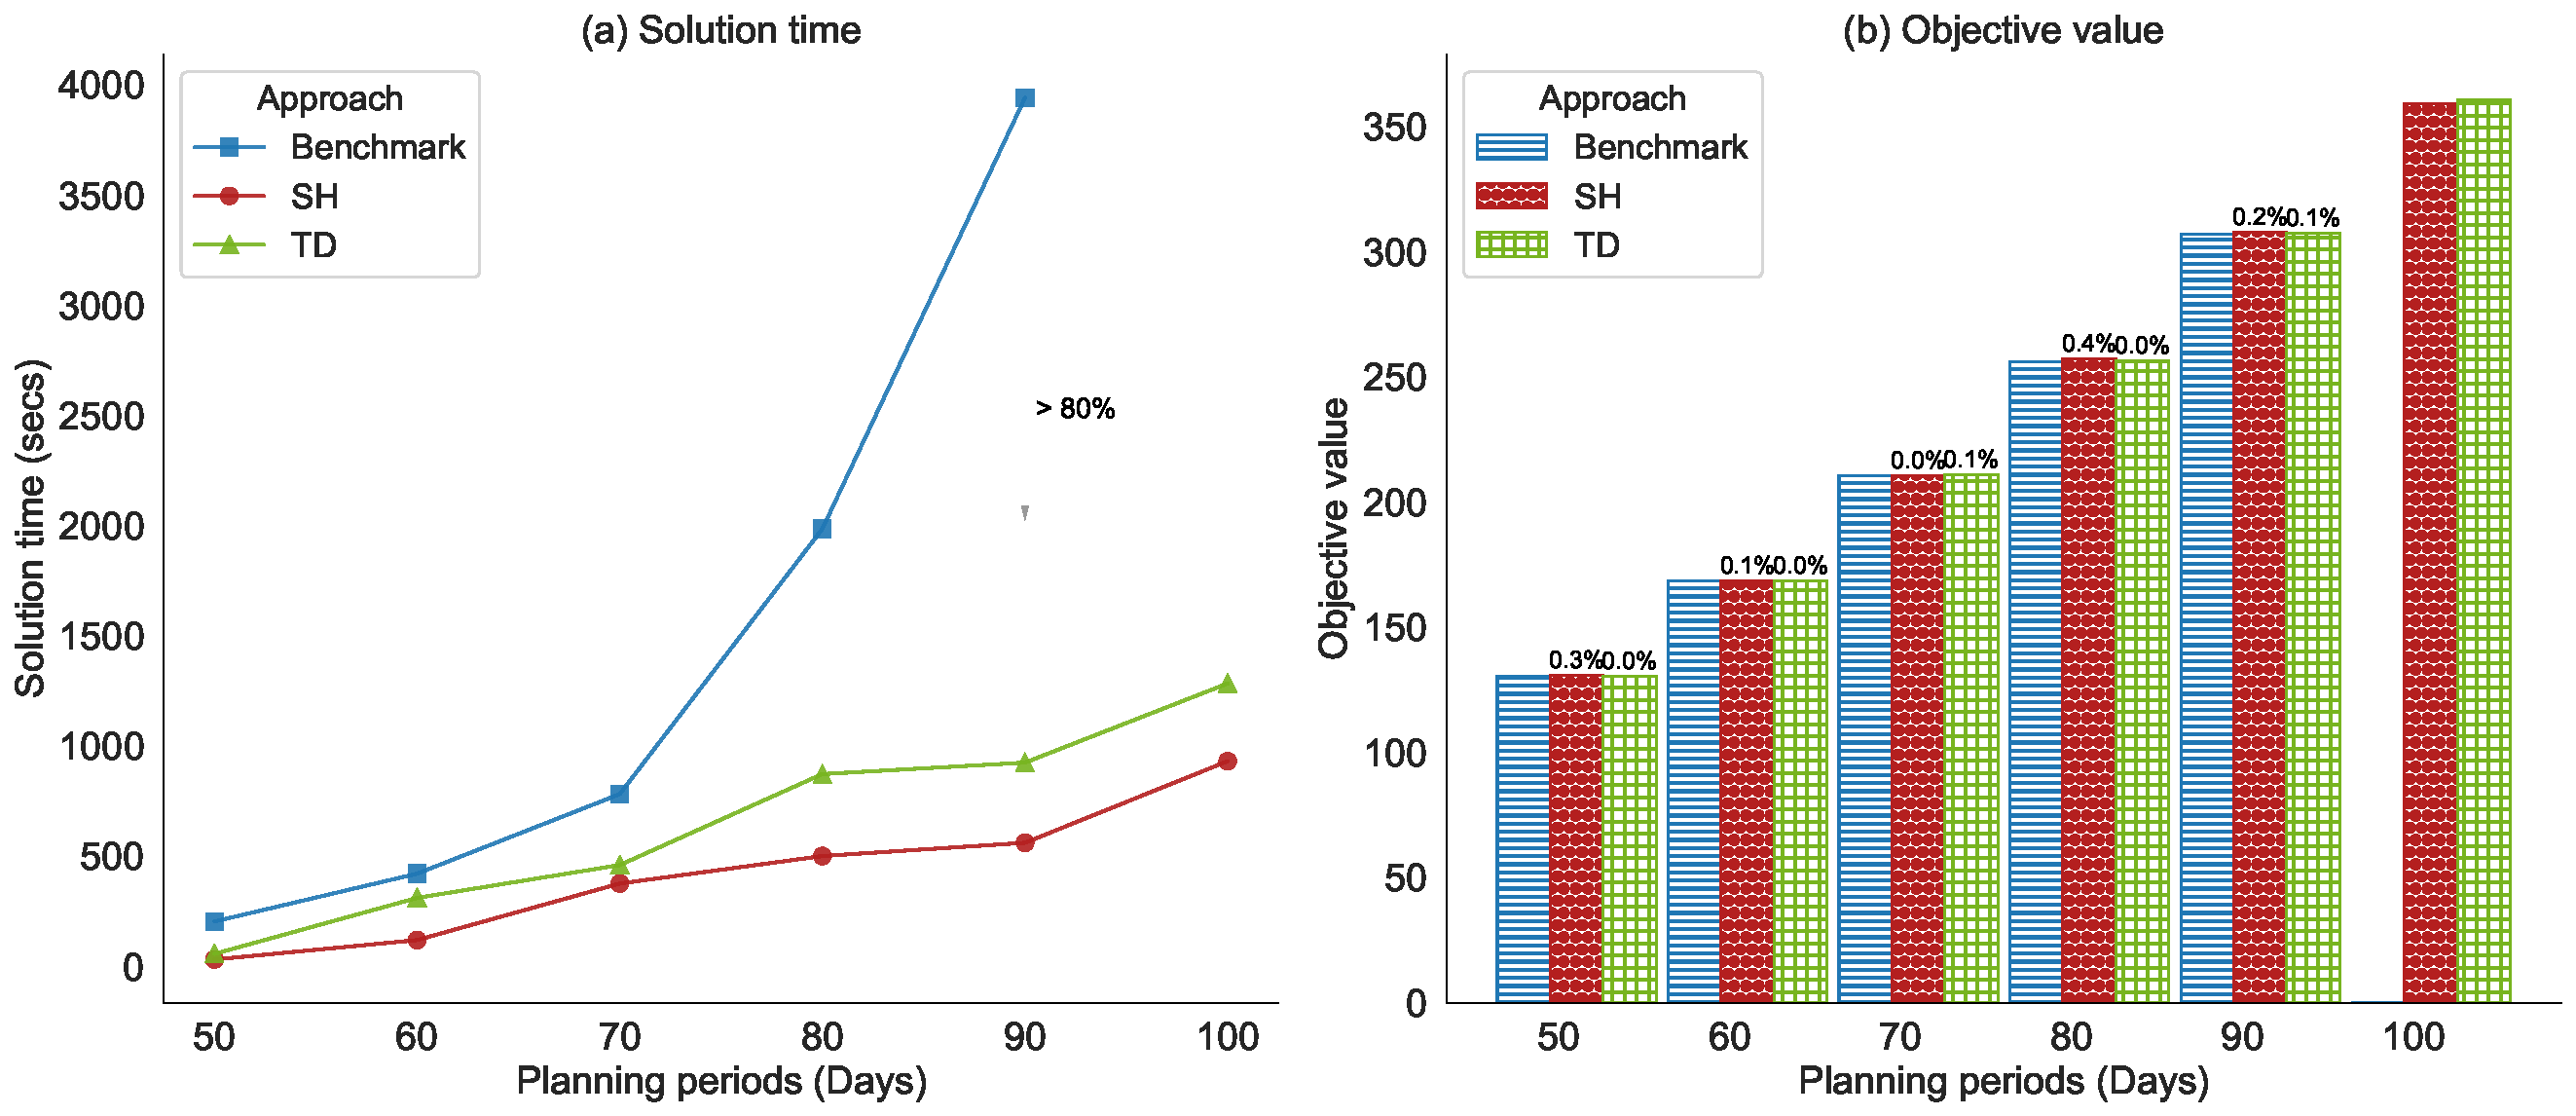
\includegraphics[width=\linewidth]{comb_compS1_v1.pdf}
    \caption{Comparison of three solution approaches under Scenario 1}
    \label{fig:comparisonS1}
\end{figure}

\begin{figure}[htbp]
    \centering
    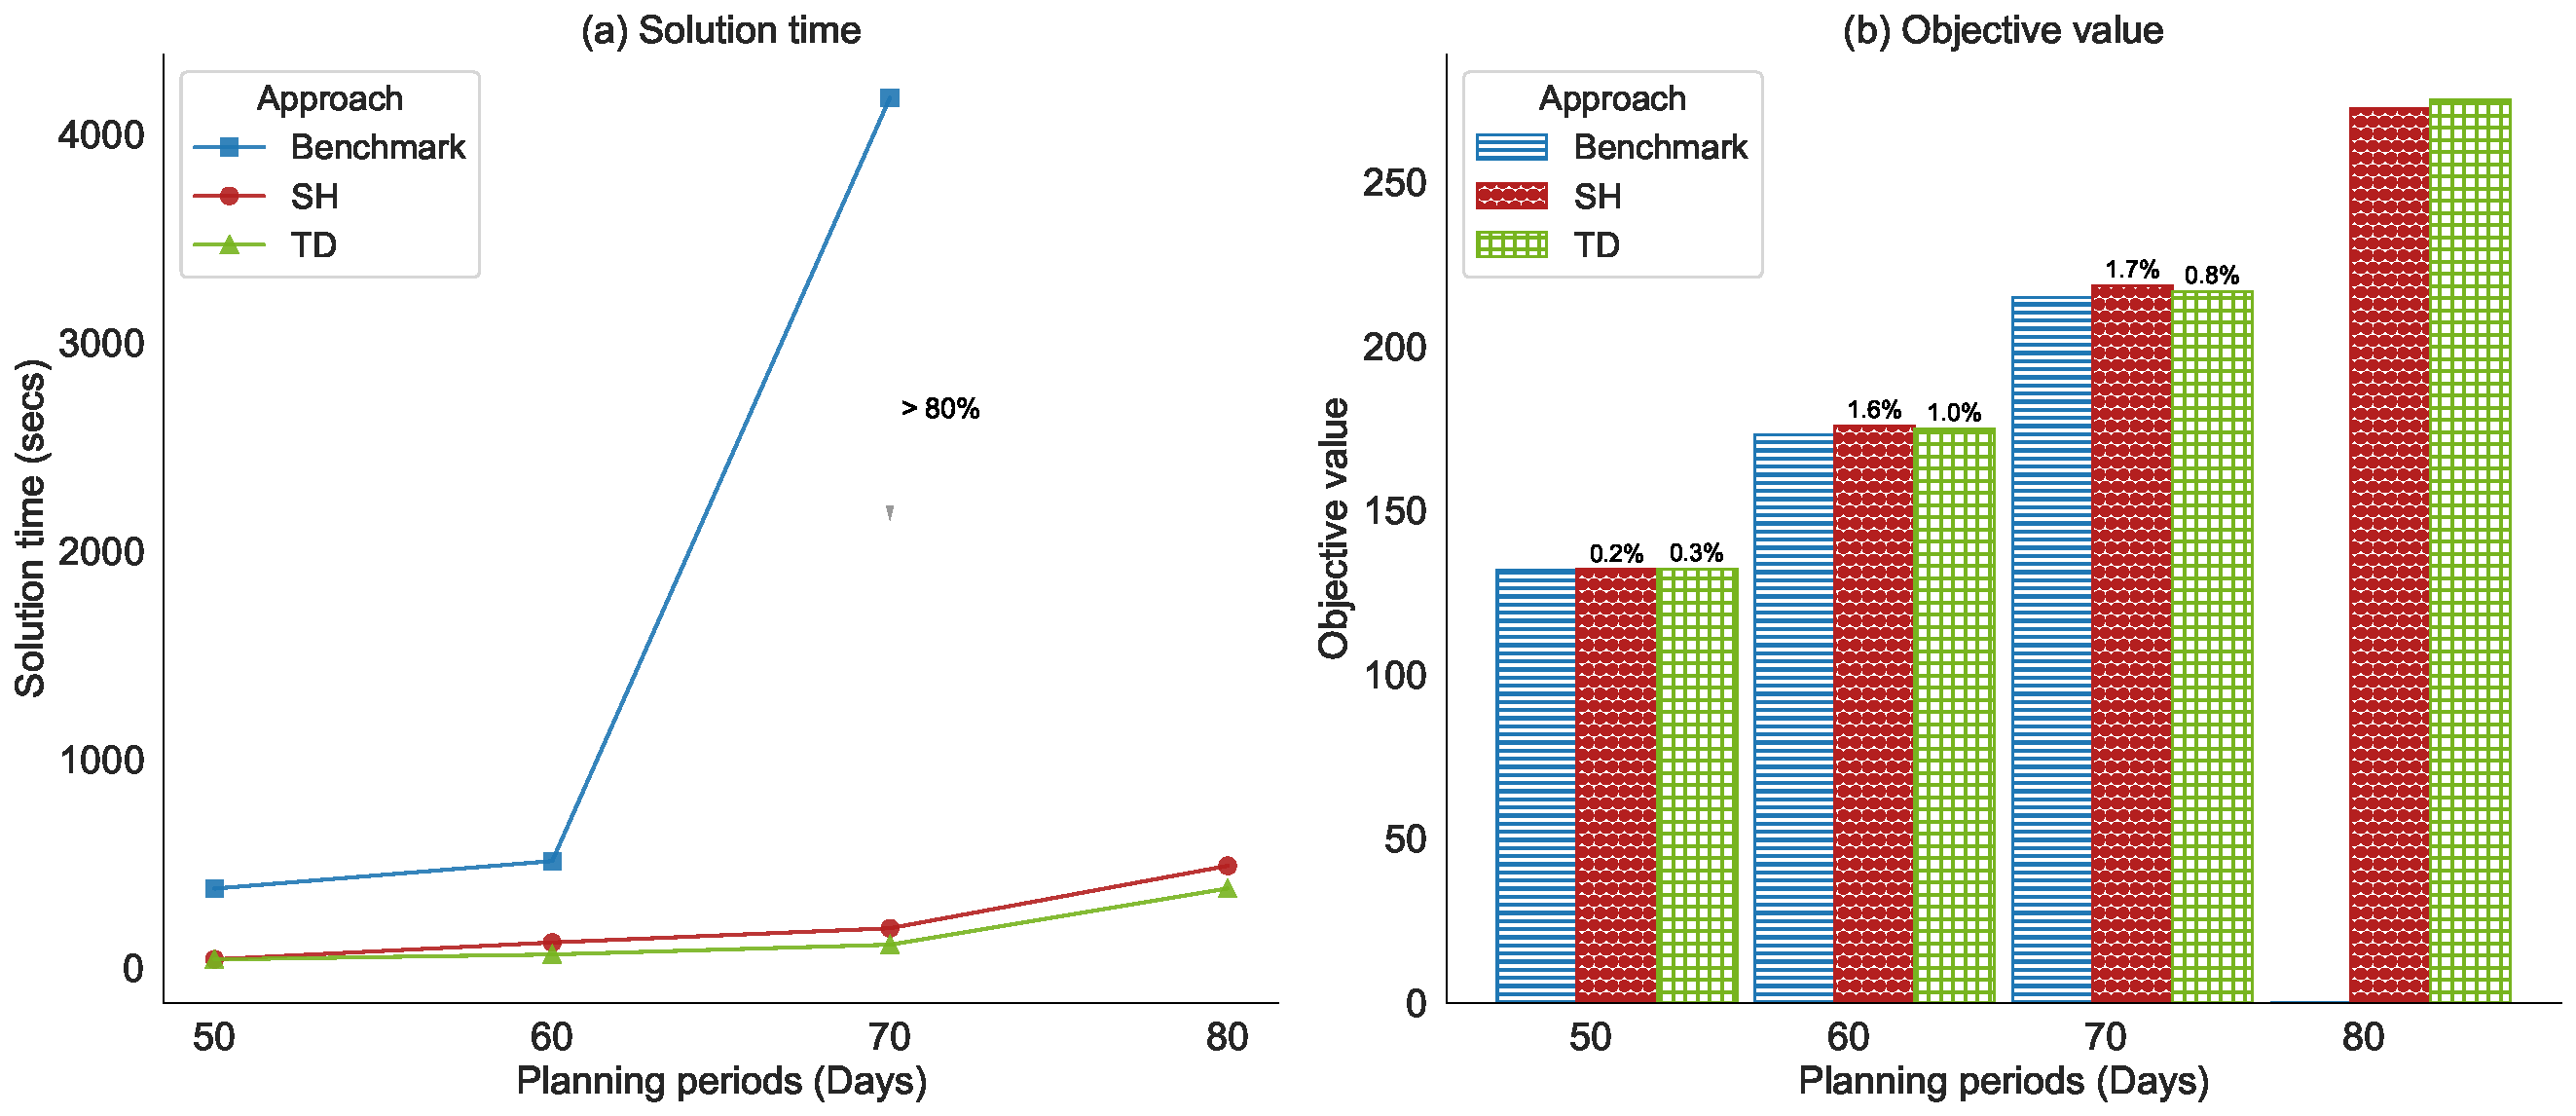
\includegraphics[width=\linewidth]{comb_compS4_v1.pdf}
    \caption{Comparison of three solution approaches under Scenario 4}
    \label{fig:comparisonS4}
\end{figure}


We next explain why the relative difference in the optimization objective seems very little, first with a toy example. Assume that there is a single tuple for maintenance at the only station. The optimal decision is to schedule it for day $t\prime$ and an alternative decision is to have the maintenance on day $t\prime-n$. The absolute cost difference due to the premature scheduling is $\gamma^{t\prime-n} - \gamma^{t\prime}$ and the relative cost change is given by $\frac{1}{\gamma^n} - 1$. Assuming $\gamma = 0.99$, the relative difference is 1.0\% when $n = 1$ and 5.2\% when $n = 5$. Similarly, in case of multiple tuples, when each tuple is scheduled one day earlier, the relative cost difference is about 1.0\%. However, one useful day from the previous check could be worth hundreds of or even thousands of dollars. AA is thus interested in comparing solutions in terms of useful day losses. 

We next introduce two concepts for a tuple $w$, namely schedule deviation $\xi_w$ and normalized schedule deviation $\bar{\xi}_w$. $\xi_w$ is computed as follows:
\begin{equation}
    \xi_w =  t_w - t_w^*, \quad \forall w \in W,
\end{equation}
where $t_w^*$ is the optimum maintenance day for tuple $w$ and $t_w$ is an alternative day suggested by a heuristic approach. Clearly, when two approaches schedule a tuple on the same day (i.e.,  $t_w = t_w^*$), the scheduling deviation is stated to be zero; further, when $t_w < t_w^*$, the scheduling difference is stated to be negative (premature maintenance); when $t_w > t_w^*$ the scheduling deviation is positive (delayed maintenance). Note even when a heuristic produces a delayed maintenance decision, the maintenance is not overdue (i.e., the minimum DTW is greater than 0). When we further consider the tuple-specific maintenance interval $m_w$, the scheduled deviation can be normalized as follows:
\begin{equation}
    \bar{\xi}_w =  \frac{t_w - t_w^*}{m_w}, \quad \forall w \in W.
\end{equation}

We next focus on the 70-day planning horizon under Scenario 4. First, all three approaches, i.e., benchmark, SH, and TD, have yielded the same number of scheduled tuples over the planning horizon. However, the maintenance schedules are different.

Figure~\ref{fig:sched_deviation} shows $t_w^*$ and $t_w$ for each scheduled tuple for both the SH and TD approaches. As multiple tuples could be scheduled on the same day, the size of each point in Figure~\ref{fig:sched_deviation} indicates the number of tuples. In other words, one point corresponds to one or multiple scheduled tuples. We can observe that most points fall either on the 45-degree line (i.e., indicating no schedule deviations) or lie close to the 45-degree line, indicating little schedule deviations. Additionally, Figure~\ref{fig:normalized_dev} shows the distribution of the normalized schedule deviation $\bar{\xi}_w$. Although $\bar{\xi}_w$ varies dramatically from -70\% to +100\%, for over 96\% of the tuples, $\bar{\xi}_w$ is within a small range, namely $-10\%$ and $+10\%$, regardless of the solution approach (SH or TD).


\begin{figure}[htbp]
    \centering
    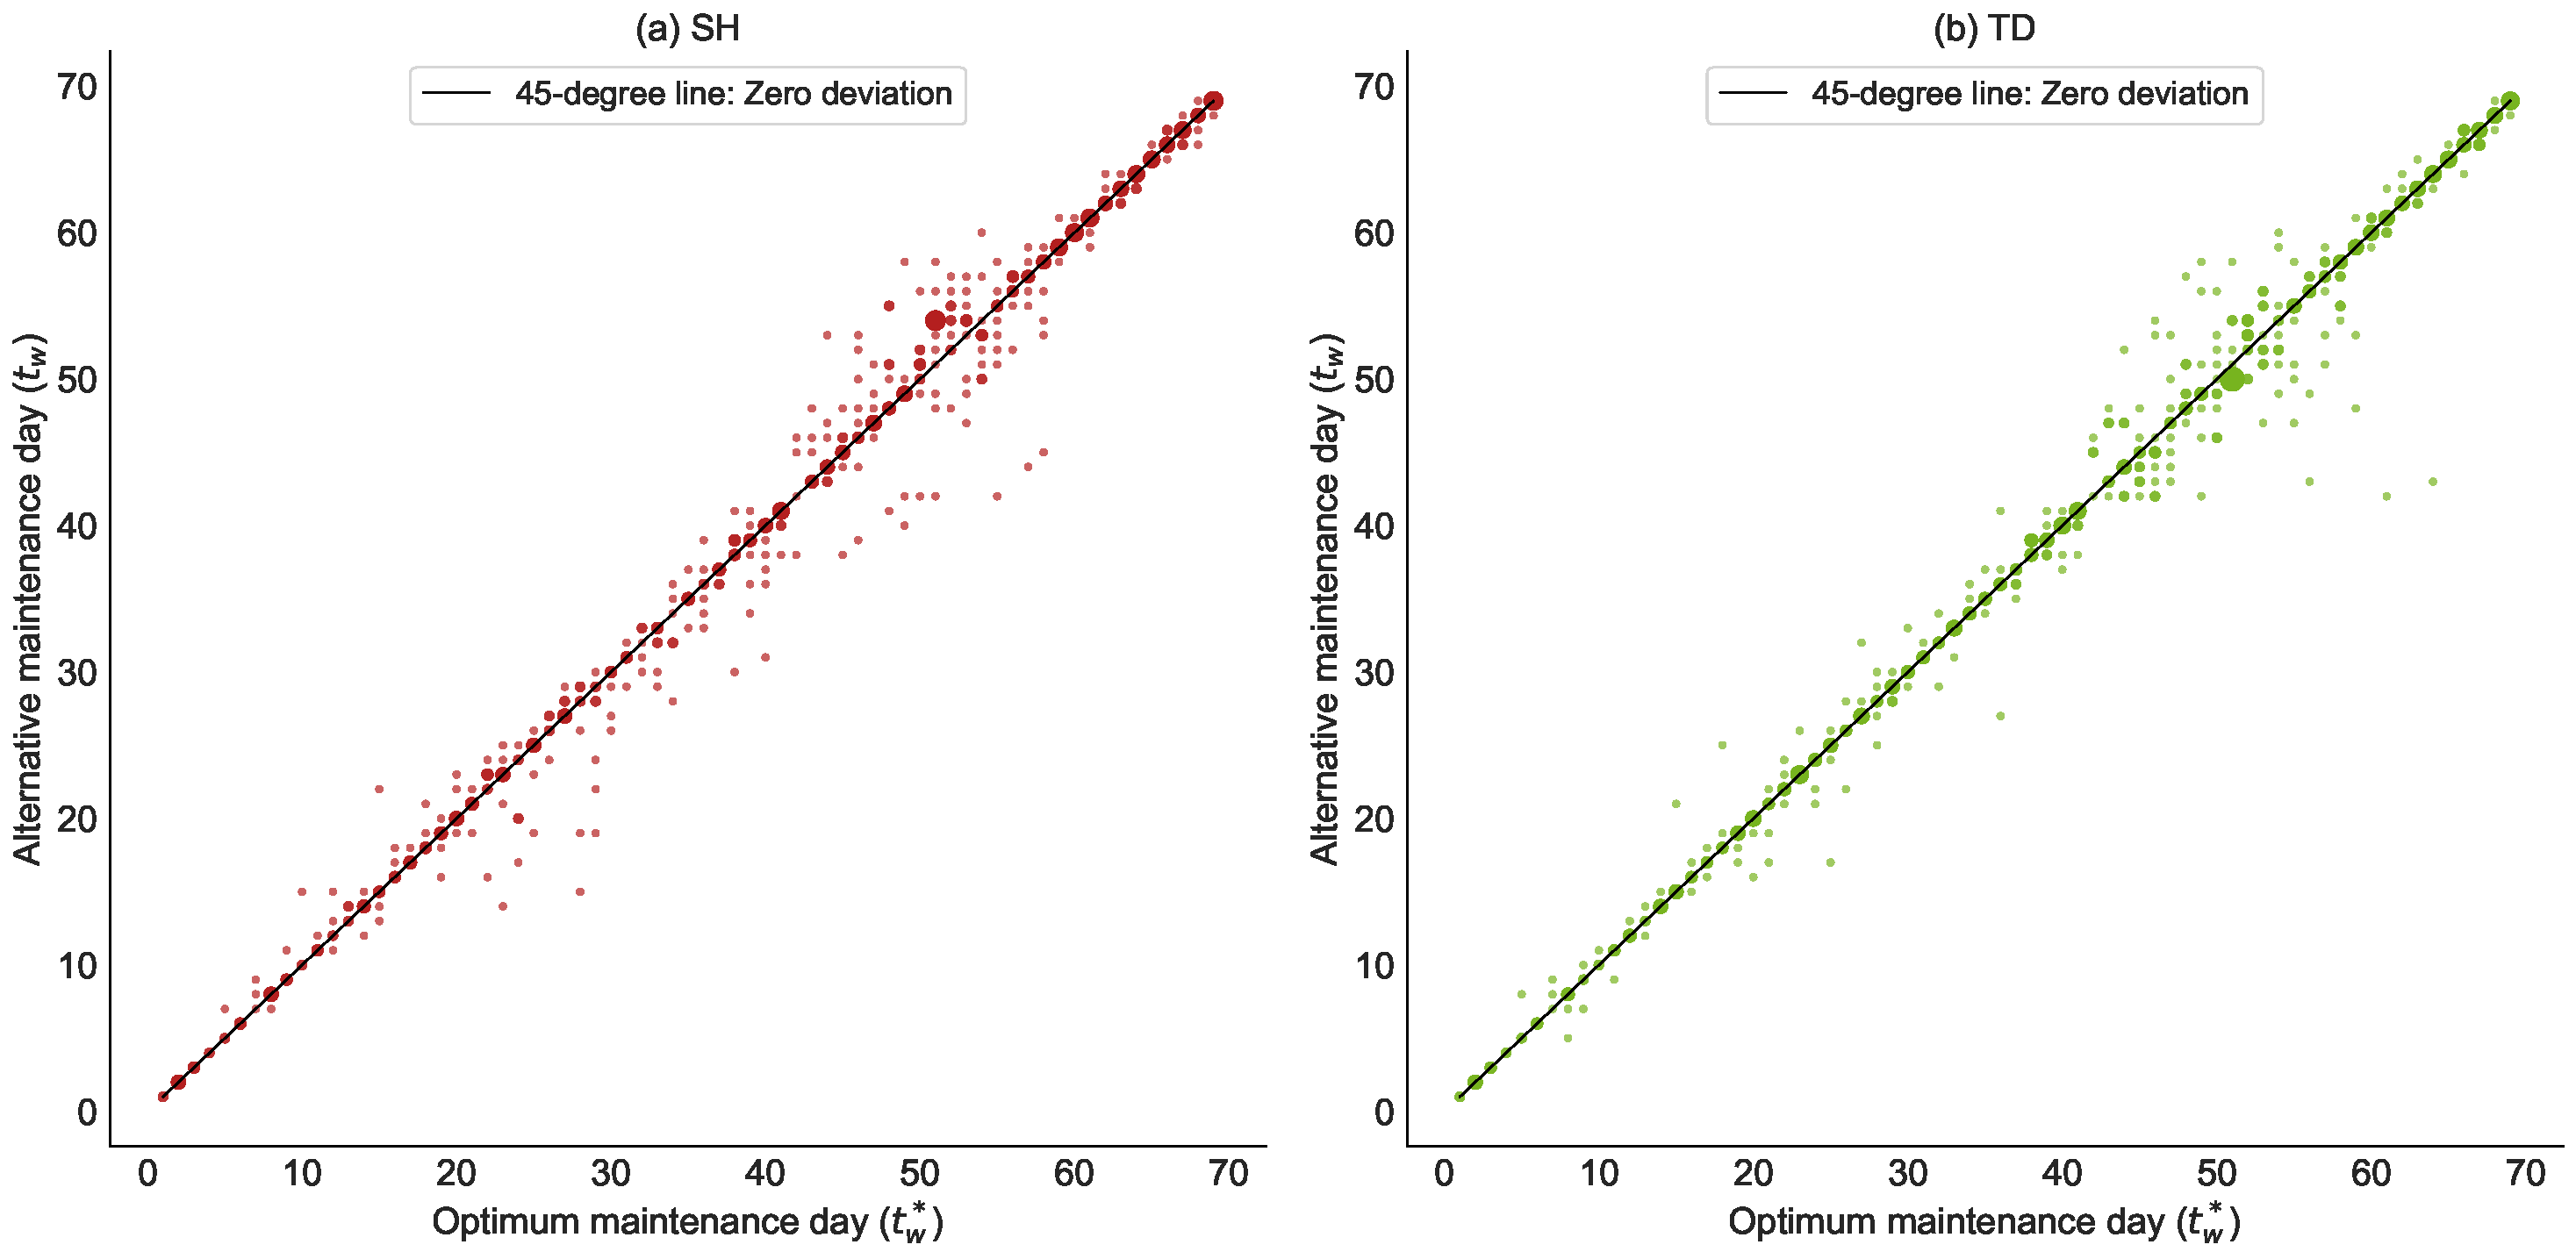
\includegraphics[width=\linewidth]{sched_dev_70.pdf}
    \caption{Scheduled deviations ($\xi_w$) for the 70-day planning horizon under Scenario 4}
    \label{fig:sched_deviation}
\end{figure}

\begin{figure}[htbp]
    \centering
    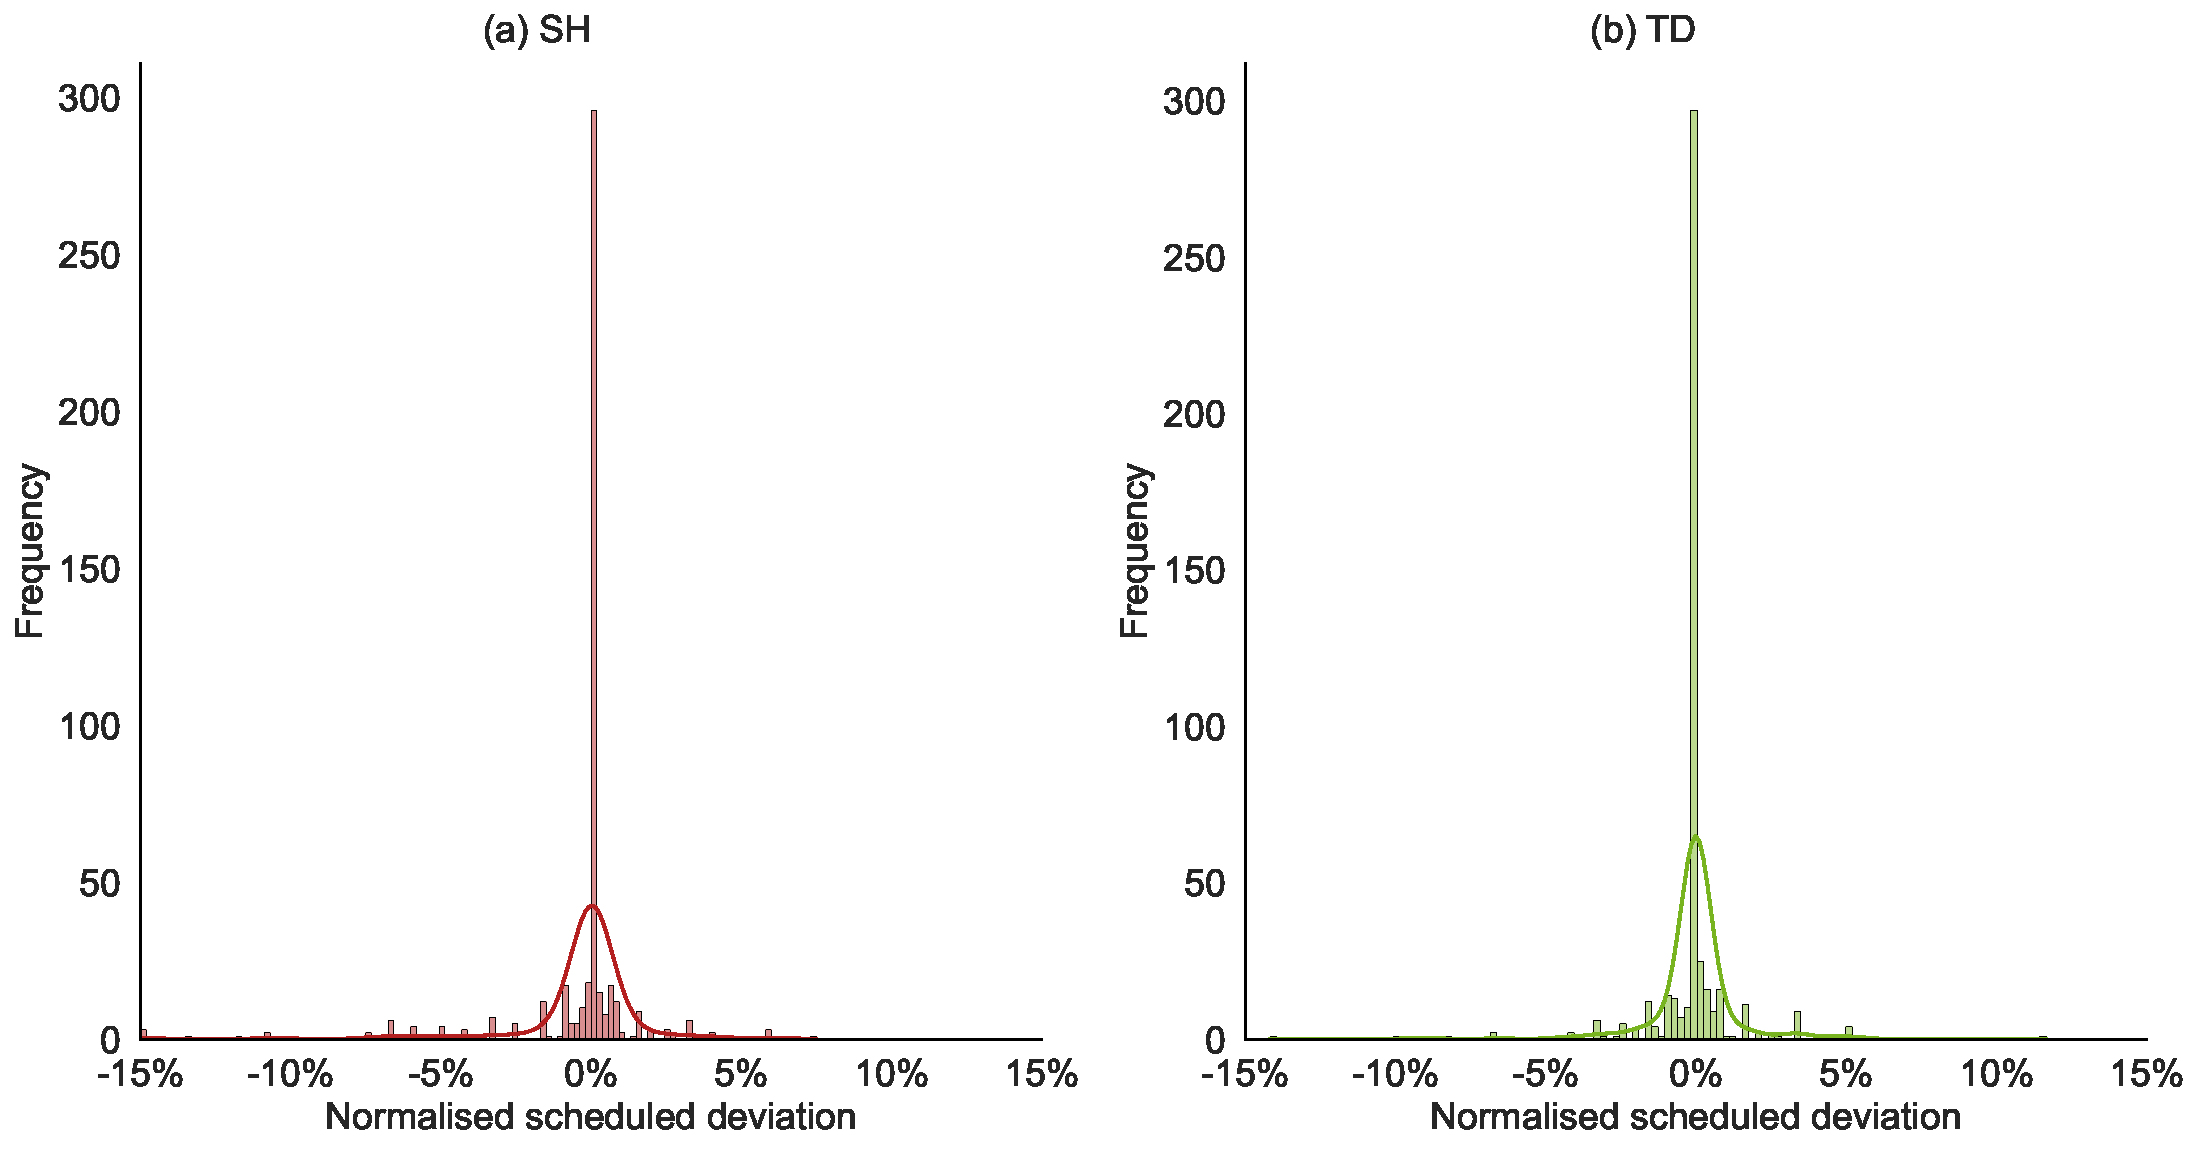
\includegraphics[width=\linewidth]{normalise_dev.pdf}
    \caption{Distribution of $\bar{\xi}_w$ for 70-day planning horizon  under Scenario 4}
    \label{fig:normalized_dev}
\end{figure}

% \begin{figure}[htbp]
%     \centering
%     \includegraphics[width=0.8\linewidth]{sched_dev.pdf}
%     \caption{Evaluation of normalized scheduled deviation $\%$ over different planning horizon lengths under scenario 4}
%     \label{fig:overal_schd_dev}
% \end{figure}

% \newpage
\subsection{A Long-term Analysis}
\label{sec:long_termAna}

After validating the high efficiency and capabilities of two decomposition-based solution approaches, we tackle a long-term planning problem. Specifically, TD is used to plan aircraft maintenance activities over a 180-day planning horizon from April 16 to October 12, 2024 assuming all stations are available (i.e., under Scenario 1). 

After pre-processing (i.e., removing tuples with very large DTGs), there are 823 aircraft and 1,631 tuples for scheduling and assignment. After solving the problem, 1,525 tuples have been scheduled, yielding a total number of 1,806 checks because a tuple could be scheduled multiple times for maintenance over the 180-day horizon. Figure~\ref{fig:schd_pertuple} shows that among 1,525 tuples, 218 tuples are scheduled for maintenance more than once (having different scheduled cycles), while the rest (1,307 tuples) are scheduled for maintenance exactly once. Notably, five tuples experience four maintenance cycles over the 180-day period. Figure~\ref{fig:schd_tuple_cycles} shows maintenance cycles for some selected tuples. Note that those four example tuples are for A checks but involve different aircraft manufacturers. For some Boeing aircraft, A checks are needed every 60 days; for Airbus, the maintenance interval for A checks could be for 120 or 150 days. Additionally, it is quite clear from Figure~\ref{fig:schd_tuple_cycles} that the DTG is not necessarily 1 when a check is scheduled.


\begin{figure}[htbp]
    \centering
    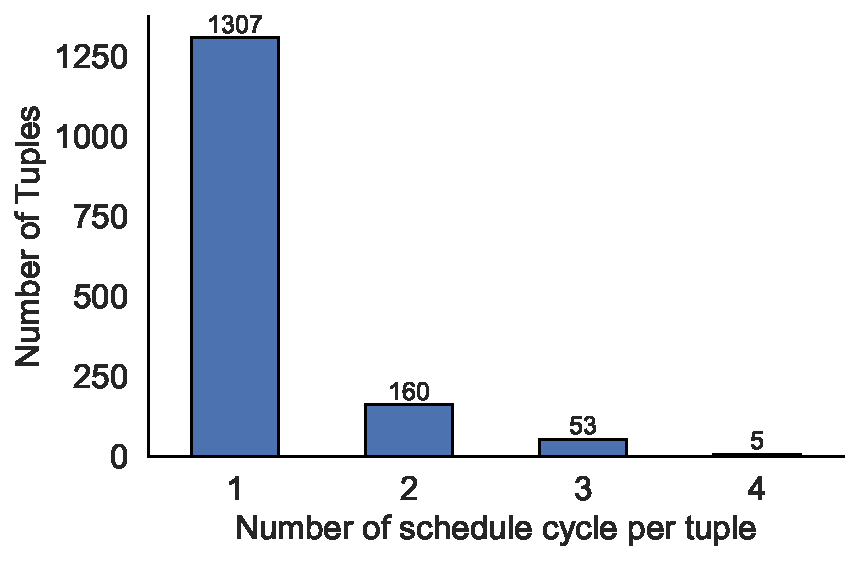
\includegraphics[width=0.5\linewidth]{Num_per_tuples.pdf}
    \caption{Distribution of the number of scheduled cycles per tuple}
    \label{fig:schd_pertuple}
\end{figure}

\begin{figure}[htbp]
    \centering
    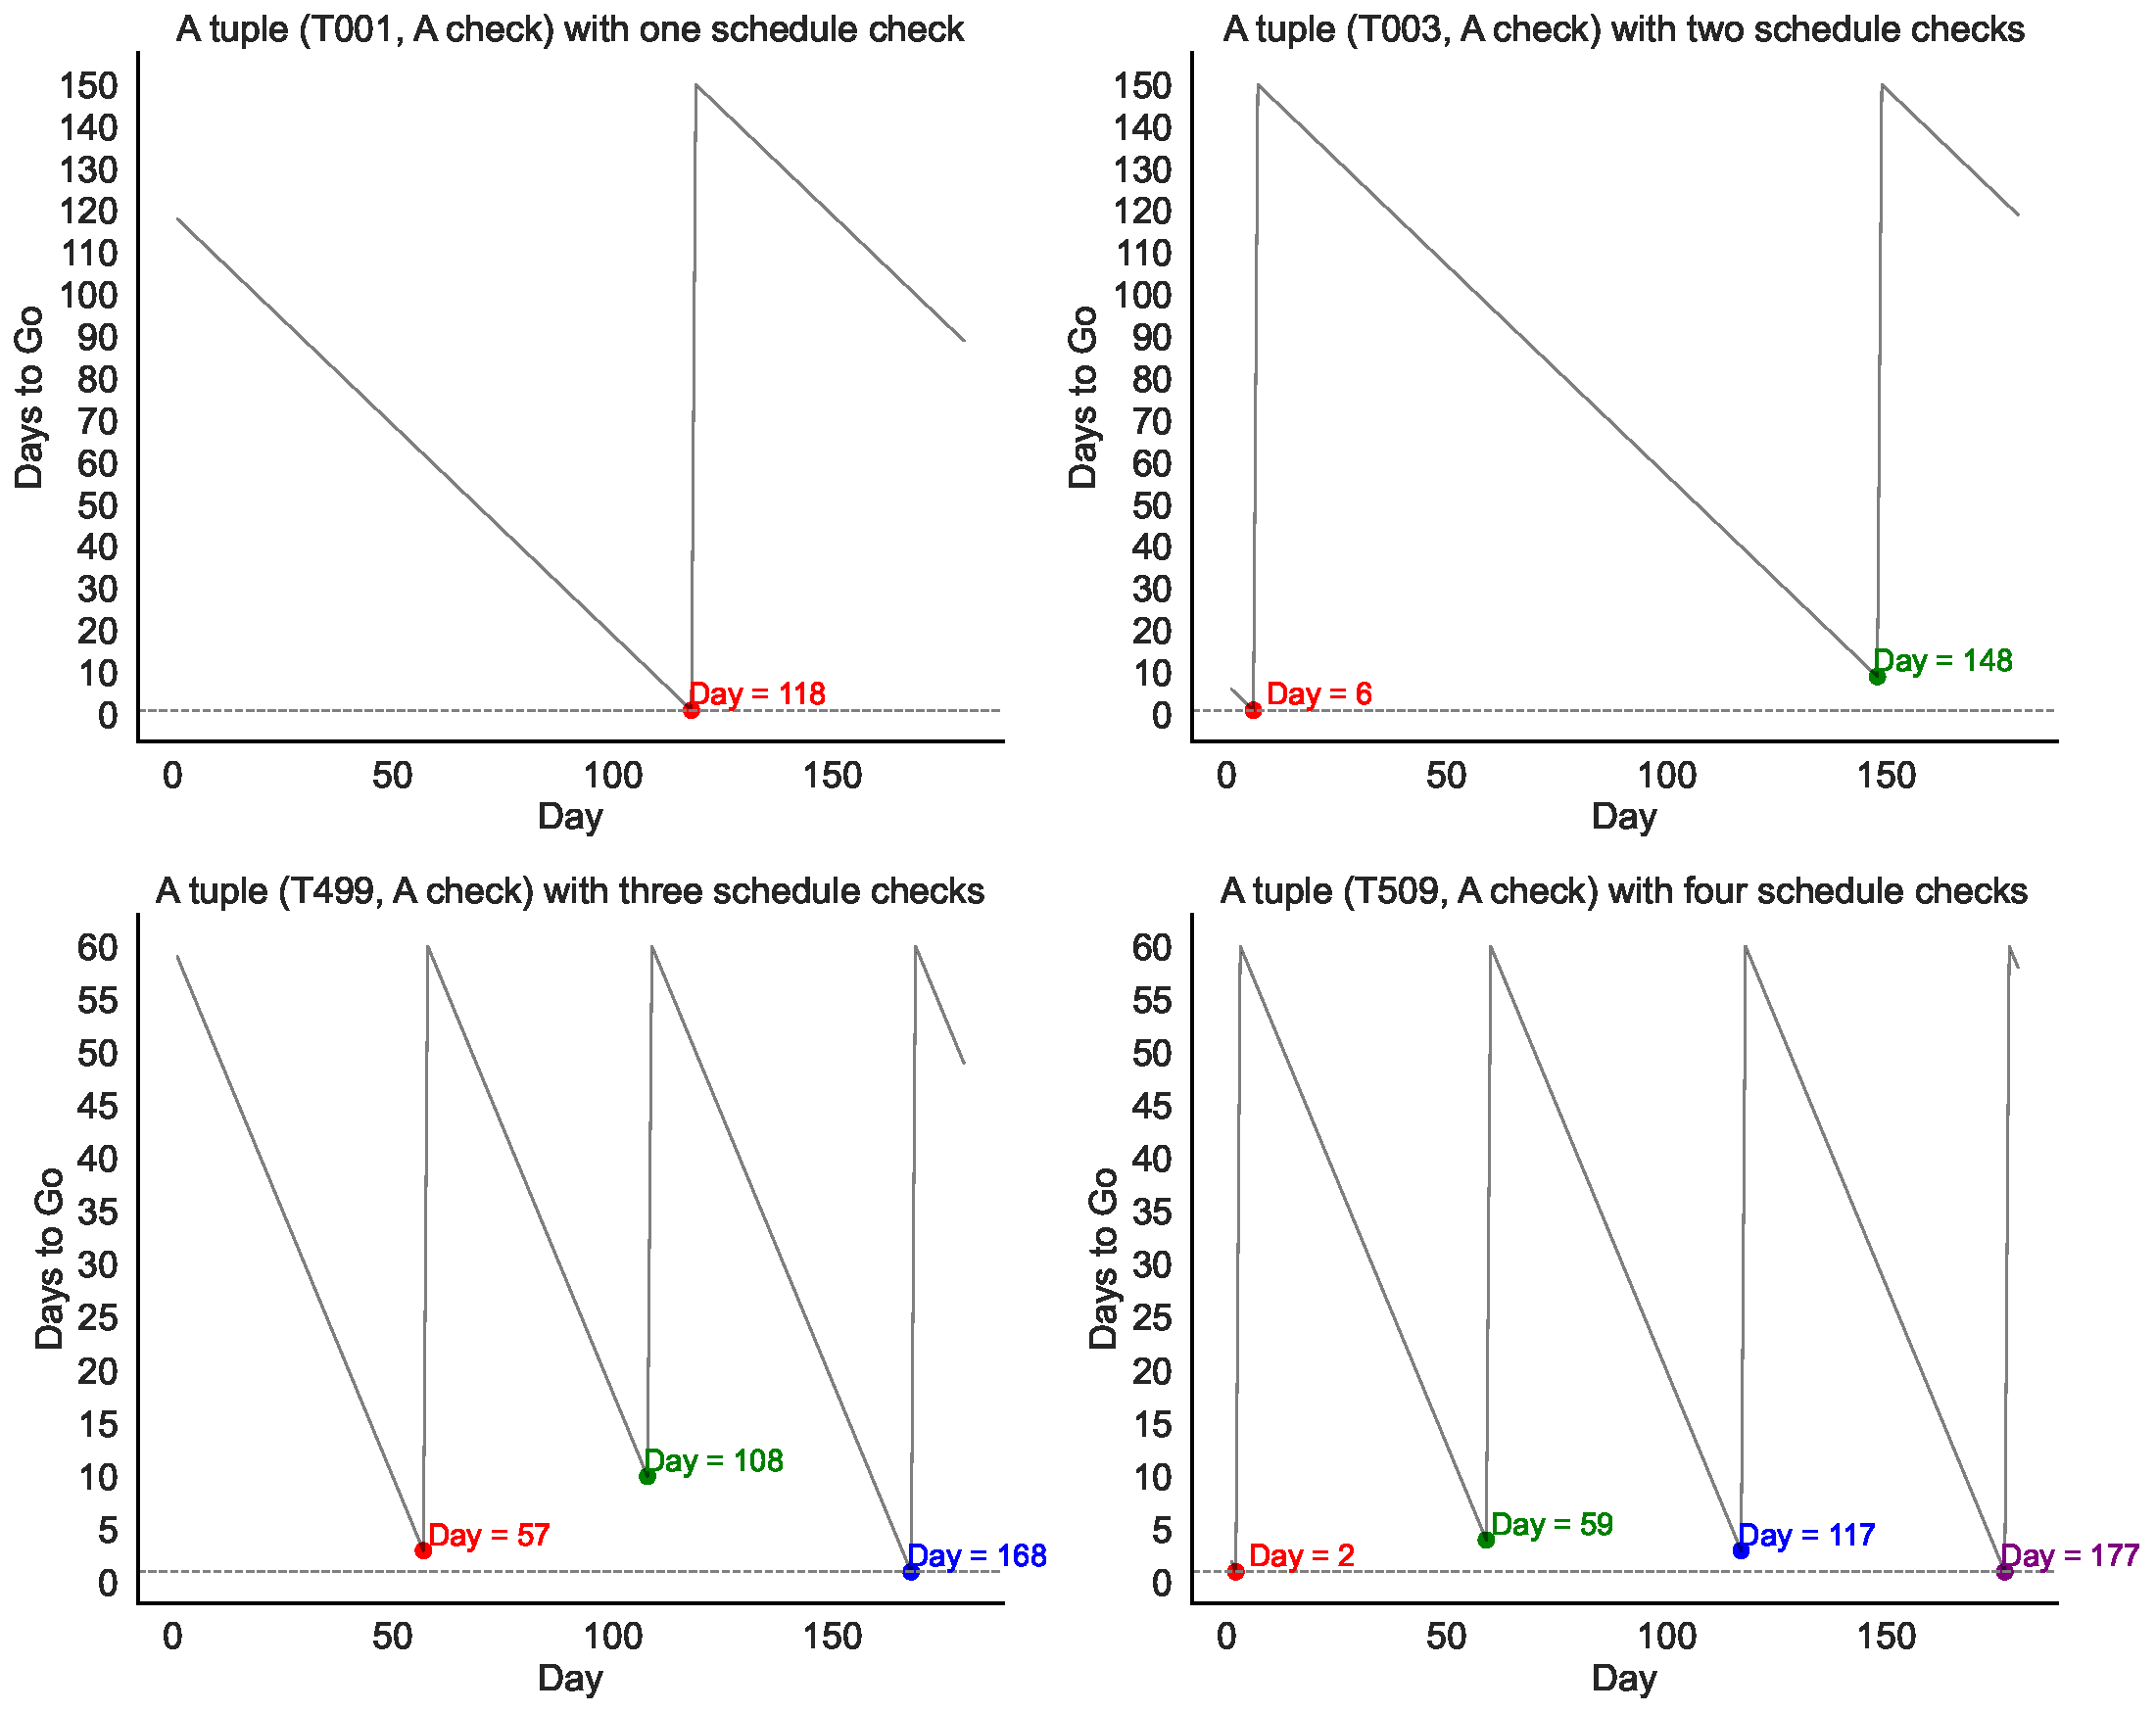
\includegraphics[width=0.9\linewidth]{schd_cycle.pdf}
    \caption{Schedule cycles for some selected tuples }
    \label{fig:schd_tuple_cycles}
\end{figure}


\begin{figure}[htbp]
    \centering
    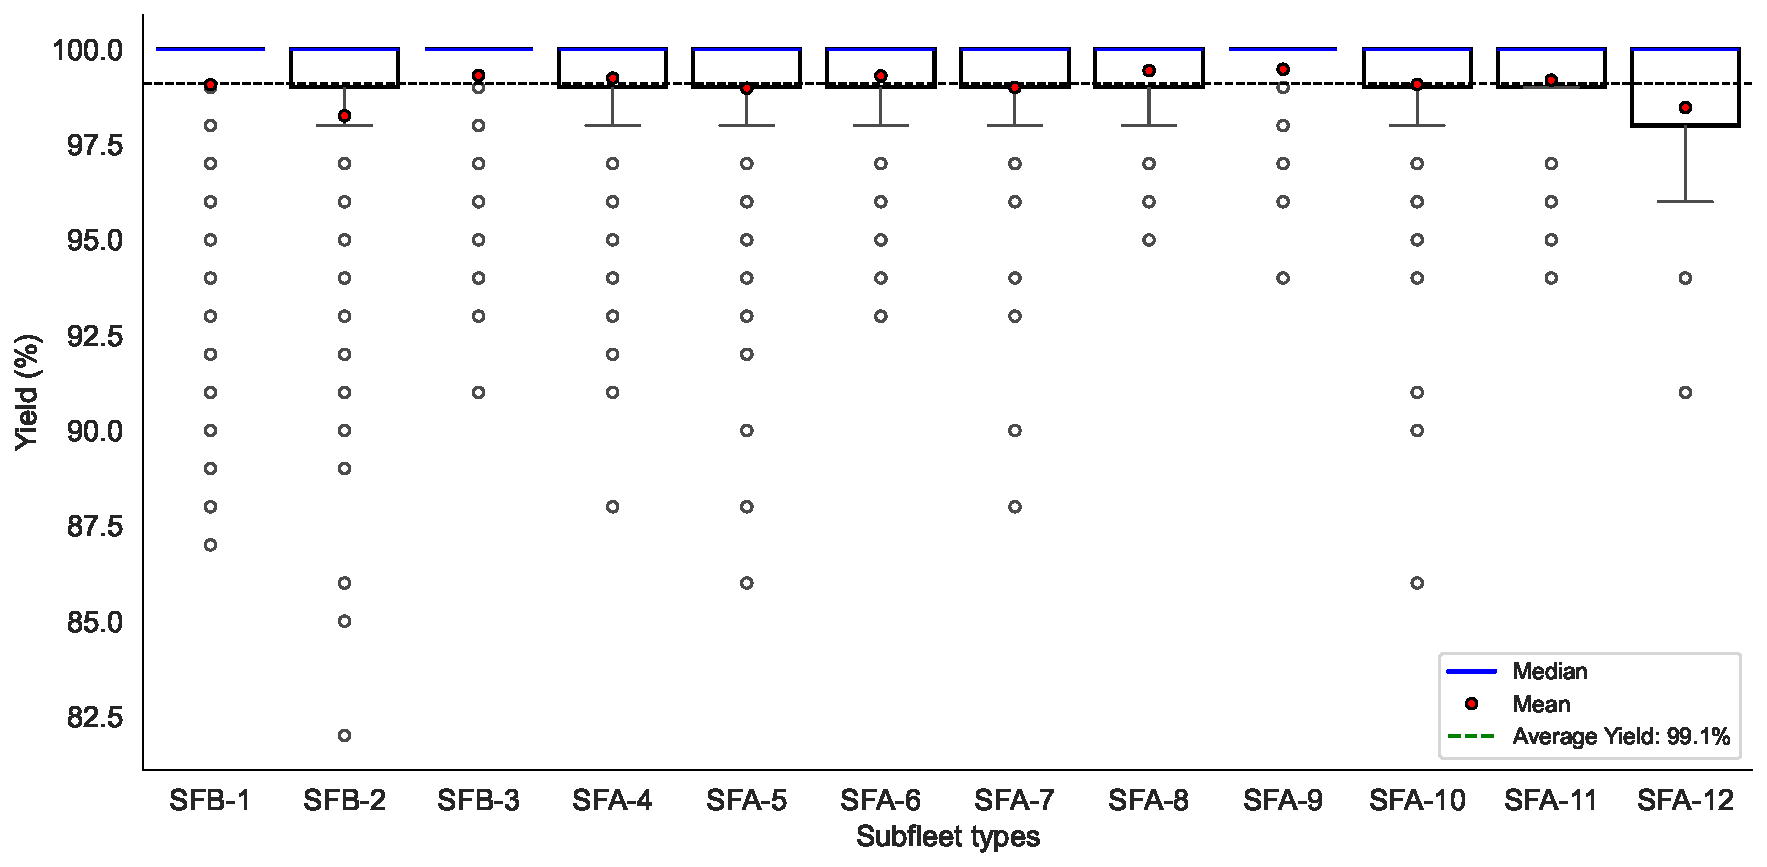
\includegraphics[width=\linewidth]{yields.pdf}
    \caption{Distribution of yield by  subfleet type}
    \label{fig:yieldist}
\end{figure}

Figure~\ref{fig:yieldist} further shows the yield distribution for each subfleet type. Recall that yield is the percentage of useful days being utilized or 100\% minus the percentage of wasted days. Generally, the yield varies from 90\% to 100\%. Note that \cite{yan2008long} explored the same concept of yield, referring to it as the \textit{aircraft use rate}, where an average value of 97.7\% was reported for their case based on a major airport in Taiwan.
Figure~\ref{fig:yieldist} also indicates that the mean variation over various subfleet types is very small, meaning that all subfleet types receive almost equal accommodation over the planning horizon (i.e., no subfleet types are being discriminated).

It is noted that the total computation time for this 180-day analysis is around 1.5 hours.


\subsection{One Application in Aircraft Maintenance Capacity Planning}
\label{sec:twoHolidays}
We next present one application of the developed long-term aircraft maintenance planning model. Specifically, we focus on two major holidays within the 180-day planning horizon: Independence Day and Labor Day. For each holiday, we anticipate a two-week travel period characterized by increased aircraft utilization and nearly no time for conducting maintenance. To model this effect, we reduce the number of aircraft accessing each maintenance station to zero for all subfleet types. In other words, all maintenance stations are effectively shut down and no maintenance activities are scheduled during these periods. We then evaluate how such an adjustment affects maintenance costs during each travel peak period.

\begin{figure}[htbp]
    \centering
    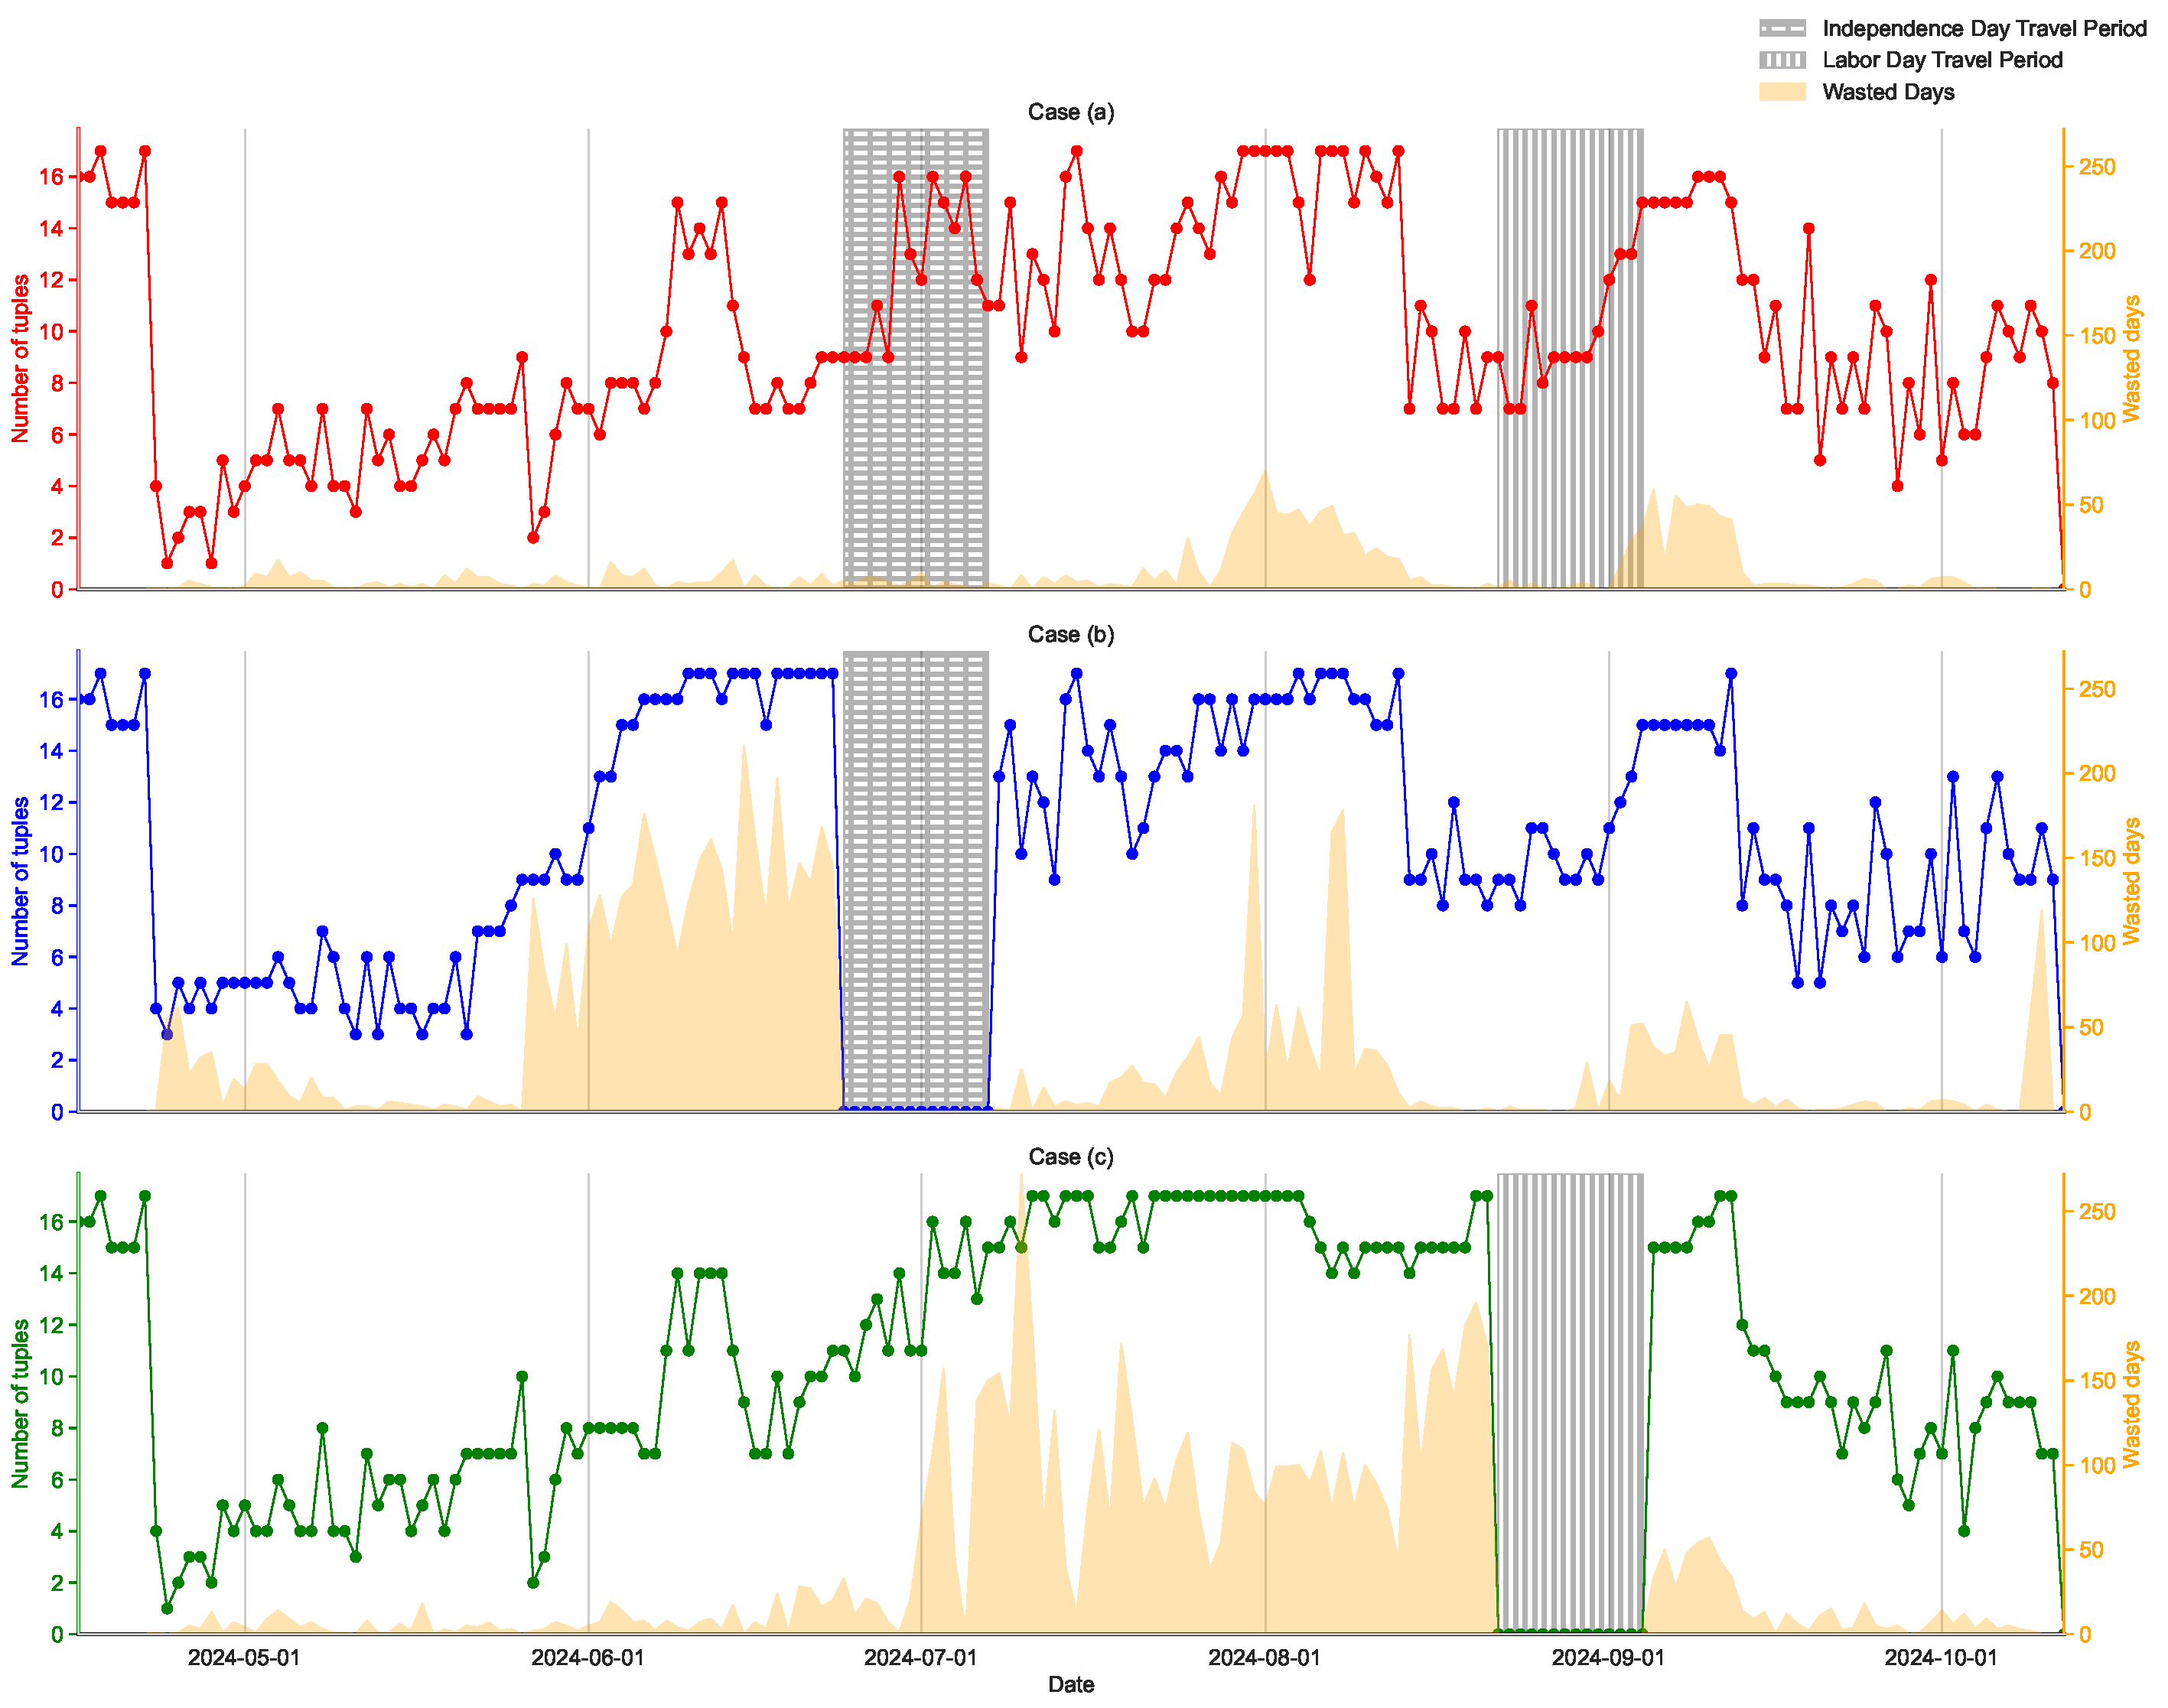
\includegraphics[width=\linewidth]{Effect_hol_red_v1.pdf}
    \caption{Effect of reduced station access during a two-week-long holiday travel period}
    \label{fig:effect_holiday_reduction}
\end{figure}

Figure~\ref{fig:effect_holiday_reduction} shows the number of scheduled tuples by day for each of the following three scenarios: (a) without any station access reductions, (b) with station access reductions only during the Independence Day travel period, and (c) with station access reductions only during the Labor Day travel period. For either holiday travel period, we observe that a large number of maintenance checks are conducted prematurely, in anticipation of the zero station access during the holiday travel period. Those premature maintenance checks imply significant economic costs. For tuple $w$, if maintenance is conducted  one day earlier than the due date (meaning that the DTG on the day of maintenance is two), the economic loss is estimated as $\frac{c_w}{m_w}$, where $c_w$ is the one-time maintenance cost for tuple $w$. Assuming that a C-Check costs \$250,000 \citep{ackert2010basics} and is good for 100 days, the economic loss of premature maintenance by a single day is thus \$2,500. Based on the wasted days visualized in Figure~\ref{fig:effect_holiday_reduction}, one can estimate the economic impact of closing maintenance stations in a travel peak period.


Table~\ref{tab-impact_sta_redu}  quantifies these impacts,  showing that due to the lack of station access during the holiday travel period, the weighted maintenance cost (namely the optimization objective) increases by 5.7\% for Independence Day and 6.1\% for Labor Day. As discussed in Section~\ref{performance_decomp}, those substantial percentage changes indicate significant wasted maintenance days. For instance, for the Labor Day travel period, the total number of wasted days across the entire fleet increases from 1,618  days to 6,595 days by 307.6\% or from approximately 0.9 days to 3.7 days per scheduled check. Another related metric also measures the significant impact of the holiday shut down on maintenance schedules. Table~\ref{tab-impact_sta_redu} shows that the average yield drops by 2.3\% and 3.6\% for the Independence Day and Labor Day, respectively. Given the above analyses of several key metrics, we conclude that the lack of station access during the Labor Day travel period has a larger impact on the maintenance plans. This also implies that if maintenance stations need to be closed for any reasons (such as for renovation), they should be closed during the Independence Day period rather than the Labor Day period to mitigate the impact on aircraft maintenance activities.

\begin{table}[htbp]
\centering
\caption{Impact of station access reductions during holiday travel periods on maintenance operations}
\label{tab-impact_sta_redu}
\resizebox{0.9\columnwidth}{!}{%
\begin{tabular}{@{}lccccc@{}}
\toprule
Cases & Objective value & \begin{tabular}[c]{@{}c@{}}$\%$ of premature \\ checks \end{tabular} & \begin{tabular}[c]{@{}c@{}}Total \\ wasted days\end{tabular} & \begin{tabular}[c]{@{}c@{}}Av. premature \\ days\end{tabular} & Av. yield \\ \midrule
Case (a) & 842.1 & 29.1$\%$ & 1,618 & 0.9& 99.1$\%$ \\
Case (b) & 889.9 & 44.1$\%$ & 6,087 & 3.4 & 96.7$\%$ \\
Case (c) & 893.1 & 48.3$\%$ & 6,595 & 3.7 & 95.4$\%$ \\ \bottomrule
\end{tabular}%
}
\end{table}


\subsection{Managerial Insights}
The case studies presented earlier yield the following important managerial insights:

\begin{enumerate}
    \item \textbf{Necessity and benefit of joint optimization.} Due to the close interrelationship between scheduling and station assignment decisions, each major airline with multiple spatially distributed maintenance bases finds it essential to jointly determine when and where to conduct maintenance for each aircraft. The joint decision-making has also been shown to be more advantageous, given its lower overall maintenance cost than the scheduling-first-assignment-second approach.
    \item \textbf{Impact of maintenance capacity.} Computational experiments indicate that when maintenance capacity is ample, airlines can schedule checks very close to their due dates to achieve almost perfect yields. By contrast, when capacities are tightly constrained, suboptimal and premature maintenance plans result. These findings suggest that aircraft maintenance operations managers should proactively manage maintenance facility capacities considering the maintenance demand of their fleets. 
    \item \textbf{Efficiency of the proposed decomposition strategies.} Although both proposed solution approaches have been proven effective, we note that the temporal decomposition approach should be appealing to aircraft maintenance planners in practice, especially considering its ease of implementation. To ensure successful implementation, two key time parameters of the rolling horizon framework should be carefully selected, and aircraft rotation requirements must be checked appropriately when transitioning from one time horizon to another
\end{enumerate}

\color{black}


\section{Conclusions}
\label{section:conclusions}
\subsection{Summary of Research Findings}
Although existing long-term aircraft maintenance planning studies have considered scheduling decisions, none of them have considered aircraft-to-station assignment, which remains a concern for a major airline with a large fleet of heterogeneous aircraft and a set of spatially distributed maintenance facilities. 
Motivated by this important research gap, we presented an integrated aircraft maintenance planning model over an extended planning horizon.  Given that directly solving the integrated optimization problem with a commercial integer programming solver is impractical for extended planning periods (e.g., six months) or under tight capacity constraints, we proposed two decomposition-based heuristics. The first solution approach separates assignment decisions from scheduling decisions, while considering the effect of scheduling decisions on assignment decisions. The second approach addresses scalability by introducing a temporal decomposition strategy that divides the extended planning horizon into partially overlapping time horizons. To mitigate the infeasibility and sub-optimality issues inherent in temporal decomposition, we carefully selected the time horizon and rolling period parameters using a grid search.
 
With real-world data support from a major U.S.-based airline, we first solved the joint optimization problem, when the planning horizon is short, with a commercial solver under a full-capacity scenario and then examined the impact of capacity reductions on aircraft maintenance planning decisions. Further, we evaluated the performance of two proposed solution approaches by comparing them with directly solving the joint optimization problem with a commercial solver. Our results show that both proposed solution approaches (i.e., SH and TD) can reduce the computational time by more than 80\%, with only minimal degradation in the optimization objective (no more than 2\%). Such small differences in the objective value are also validated by examining the absolute and relative schedule deviations. We find that the schedule deviations are zero for most of the tuples, although substantial deviations can be observed for a very small percentage of tuples. Therefore, we conclude that both SH and TD can strike preferable trade-offs between solution time and quality.

Due to the highly satisfactory performance of the proposed solution approaches, we were able to conduct a long-term analysis spanning 180 days. One notable finding is that our proposed optimization method can schedule a tuple for maintenance over a long planning horizon multiple times, which is a key feature desired by the anonymous airline while being missed in the literature \citep{yan2008long}. Finally, we demonstrated the practical relevance of such a long-term aircraft maintenance planning model by analyzing the impact of station access reductions during anticipated travel peaks.


\subsection{Practice Significance of this Study}
Our research was conducted in response to the practical needs of AA. The current long-term aircraft maintenance planning practice is largely manual and based on planners’ experience, similar to what was described by \cite{boere1977air}. To replace the time-consuming and labor-extensive process, internal consultants developed some integer programming models; however, one of the major shortcomings was that over a planning horizon, a single check can be scheduled for each aircraft, while it is highly desirable for AA that a series of checks could be scheduled over time. With that clear research need to be addressed, we presented a joint optimization model and two effective decomposition-based solution approaches, as described in earlier sections of this paper. Therefore, this study is expected to advance the current practice in at least two ways: first, it can replace the current labor-extensive aircraft maintenance planning process and yield more favorable maintenance plans; second, it enhances the current optimization methods developed by the internal consultants at AA and thus becomes a cornerstone of their next-generation computer-based aircraft maintenance scheduling system.



\subsection{Research Extensions}
The current research presented in this paper can be improved or extended in multiple ways, including:
\begin{enumerate}
    \item In a long-term planning problem, the inherent uncertainty about maintenance station capabilities or capacities should be considered \citep{sun2015stochastic}. The possibility of rescheduling in anticipation of flight cancellations or other disruptions should be incorporated. 
    \item In addition to managing aircraft maintenance demand, maintenance capacity planning can be conducted at the same time. For instance, the timing of a major renovation for a maintenance station can be carefully selected to avoid major impacts on aircraft maintenance schedules. 
    \item The training of maintenance personnel and consideration of the licensing processes for engineers could be integrated to ensure that workforce readiness aligns with the fluctuating demand of maintenance.
\end{enumerate}



\section*{Acknowledgments} 
% \noindent \textcolor{myblue}{We greatly appreciate the constructive comments from the handling editor and three anonymous reviewers.} 
% This research was partially supported by the National Science Foundation (NSF). The views expressed in this article are solely those of the authors and do not necessarily reflect the views of the NSF. 
We gratefully acknowledge the data support provided by American Airlines and the valuable feedback from the following experts:
Dr. Patrice Yapo, Principal Operations Research Consultant, Operations Research \& Advanced Analytics (ORAA),
Dr. Irandokht Parviziomran, Consultant, ORAA,
Dr. Jose A. Ramirez-Hernandez, Senior Lead Consultant, ORAA, 
Mr. Larry Richardson, Senior Manage, Line Maintenance Capacity and Schedule, and 
Dr. Tuell Green, Managing Director, ORAA.

% \section*{Research Data}
% \noindent The data used in this article are proprietary to the industry and require authorization for release.



% \section*{CRediT authorship contribution statement}
% \noindent \textbf{JohnPaul Adimonyemma}: Conceptualization, Methodology, Visualization, Writing – original draft, Investigation, Formal analysis.  \textbf{Yanshuo Sun}: Conceptualization, Formal analysis, Project administration, Methodology, Writing - original draft, review, and editing.

% \section*{Data availability} 

% \noindent Data will be made available upon request.


\appendix


\renewcommand{\theequation}{A-\arabic{equation}}
\newpage
\bibliography{_mybibfile}
% \bibliography{reference}
 

\end{document}


